%=-=-=-=-=-=-=-=-=-=-=-=-=-=-=-=-=-=-=-=-=-=-=-=-=-=-=-=-=-=-=-=-=-=-=-=-=-=-=-=-
% PREAMBLE
%=-=-=-=-=-=-=-=-=-=-=-=-=-=-=-=-=-=-=-=-=-=-=-=-=-=-=-=-=-=-=-=-=-=-=-=-=-=-=-=-

\documentclass[a4paper]{article}


%=-=-=-=-=-=-=-=-=-=-=-=-=-=-=-=-=-=-=-=-=-=-=-=-=-=-=-=-=-=-=-=-=-=-=-=-=-=-=-=-
% Packages
%%
%\usepackage{fullpage} % Package to use full page
\usepackage{geometry}
 \geometry{
 a4paper,
 total={170mm,257mm},
 left=20mm,
 top=20mm,
 right=20mm,
 bottom=20mm
 }
\usepackage{parskip} % Package to tweak paragraph skipping
\usepackage{amsmath} % standard
\usepackage{amssymb} % standard - Double R symbol etc.
\usepackage{hyperref}
\usepackage{amsthm} % standard - theorem, definition, etc.
\usepackage{multicol} % multiple columns for numbering
\usepackage{enumitem} % standard - enumerate styles
\usepackage[utf8]{inputenc}
\usepackage{scrextend} % indentation
\usepackage{graphicx} % add figures
\usepackage{float} % figure position
\usepackage{pifont} % symbols
\usepackage{gensymb} % degree symbol \degree
\usepackage{xcolor} % bg color
\hypersetup{
    colorlinks,
    linkcolor={black!50!black},
    citecolor={blue!50!black},
    urlcolor={blue!80!black}
}
\usepackage{framed} % bg color
\usepackage[T1]{fontenc} % small caps
\usepackage{sectsty} % headings colour
\usepackage{mathtools}% Loads amsmath
\usepackage{amsthm,thmtools,xcolor} % coloured theorem
\usepackage[toc,page]{appendix} % reference to appendix
\usepackage{titlesec} % change chapter, section, etc. formats
\usepackage{xifthen} % if, else
\usepackage{etoolbox}
% format numbering in theorem, lemma, etc. environment
\AtBeginEnvironment{theorem}{\setlist[enumerate, 1]{font=\upshape,  wide=0.5em, before=\leavevmode}}
\AtBeginEnvironment{lemma}{\setlist[enumerate, 1]{font=\upshape,  wide=0.5em, before=\leavevmode}}
\usepackage[letterspace=150]{microtype} % \textls{<letterspaced text>} % 0 <= letterspace <= 1000, 1000 = M space
\usepackage{letltxmacro} % renew commands?
\usepackage{minted} % minted package to list code
\usepackage{subfig}
\usepackage{eso-pic} % title page bg pic
%\usepackage{fouriernc} % Use the New Century Schoolbook font
\usepackage{varwidth}
%\usepackage{pgfornament} % ornaments
\usepackage[object=vectorian]{pgfornament} %%  http://altermundus.com/pages/tkz/ornament/index.html
\PassOptionsToPackage{svgnames}{xcolor}
\usepackage{tikz}
\usepackage{fourier-orns} % line ornaments
\usepackage{adforn} % line ornaments
\usepackage{fontawesome} % \faQuestionCircle
\usepackage{marvosym}%\Pointinghand
\usepackage{mdframed} % easy outline frames
\usepackage{array,booktabs,calc} % table figs and text
\usepackage{comment} % \begin{comment}
\usepackage{fancyhdr} % page headings
\usepackage{mdframed} 
\usepackage[backend=biber,sorting=none,style=ieee]{biblatex}
\addbibresource{bibliography.bib}
\usepackage{url}


%% extra comments that I don't know where they belong:
% list of ding tags: http://willbenton.com/wb-images/pifont.pdf

%=-=-=-=-=-=-=-=-=-=-=-=-=-=-=-=-=-=-=-=-=-=-=-=-=-=-=-=-=-=-=-=-=-=-=-=-=-=-=-=-
% Colours for various things
%%

\definecolor{shadecolor}{rgb}{1.,0.933,0.96} % bg color, r,g,b <= 1
\definecolor{LightPink}{rgb}{0.92.,0.8,0.84} % bg color, r,g,b <= 1
\definecolor{LighterPink}{rgb}{1.,0.94,0.97} % bg color, r,g,b <= 1
\definecolor{LightestPink}{rgb}{1.,0.97,0.99} % bg color, r,g,b <= 1
\definecolor{DarkestPink}{rgb}{0.36, 0.0, 0.18}
\definecolor{DarkerPink}{rgb}{0.41, 0.0, 0.21}
\definecolor{DarkPink}{rgb}{0.55, 0.05, 0.37}
\sectionfont{\color{DarkestPink}}  % sets colour of sections
\subsectionfont{\color{DarkerPink}}  % sets colour of sections
\subsubsectionfont{\color{DarkerPink}}  % sets colour of sections


%=-=-=-=-=-=-=-=-=-=-=-=-=-=-=-=-=-=-=-=-=-=-=-=-=-=-=-=-=-=-=-=-=-=-=-=-=-=-=-=-
% Define my own theorem styles
%%

% "base" styles
\declaretheoremstyle[
  headfont=\color{DarkPink}\bfseries,
  bodyfont=\itshape,
]{colored}

\declaretheoremstyle[
  headfont=\color{DarkPink}\bfseries,
  bodyfont=\normalfont,
]{colored_upright}

% theorems (corollaries, etc) themselves, inherit from my style above
% Usage:
% \begin{theorem} \end{theorem}, \begin{lemma} \end{lemma}, ...
\declaretheorem[
	numberwithin=section,
 	style=colored,
	name=\textsc{Theorem},
]{theorem}

\declaretheorem[
	numberwithin=section,
 	style=colored,
	name=\textsc{Corollary},
]{corollary}

\declaretheorem[
	numberwithin=section,
	style=colored,
	name=\textsc{Lemma},
]{lemma}

\declaretheorem[
	numberwithin=section,
	style=colored,
	name=\textsc{Definition},
]{definition}

\declaretheorem[
	numberwithin=section,
  	style=colored,
  	name=\textsc{Example},
]{exmp}


%=-=-=-=-=-=-=-=-=-=-=-=-=-=-=-=-=-=-=-=-=-=-=-=-=-=-=-=-=-=-=-=-=-=-=-=-=-=-=-=-
% Numberings, counters and spacings
%%
\numberwithin{equation}{section} % section number in eq/s
\setlength{\jot}{7pt} % spacing in split, gathered env/s

%%%%%%%%%%%% Unused %%%%%%%%%%%%
%% {style_name}{Header}[optional_number_to_inherit]
%% Usage: \begin{style_name}Text\end{style_name}
%% Output: <bold>Header optional_number_to_inherit.</bold>
%\newtheorem{theorem}{\textsc{Theorem}}[section]
%\newtheorem{corollary}{\textsc{Corollary}}[theorem]
%\newtheorem{lemma}{\textsc{Lemma}}[section]
%\newtheorem{definition}{\textsc{Definition}}[section]

%% Custom examples
%% Output - Example 1,2,...
\newcounter{example}
\newenvironment{example}[1][]{\refstepcounter{example}\par\medskip
   \textbf{Example~\theexample. #1} \rmfamily}{\medskip}
%%%%%%%%%%%% End of unused %%%%%%%%%%%%

%% Custom solution
\newcounter{solution}
\newcommand\TheSolution{%
	\textbf{Solution:}\\%
}


%=-=-=-=-=-=-=-=-=-=-=-=-=-=-=-=-=-=-=-=-=-=-=-=-=-=-=-=-=-=-=-=-=-=-=-=-=-=-=-=-
% Paths
%%
\graphicspath{ {./img/} } % figures' path - can look up files directly from there


%=-=-=-=-=-=-=-=-=-=-=-=-=-=-=-=-=-=-=-=-=-=-=-=-=-=-=-=-=-=-=-=-=-=-=-=-=-=-=-=-
% My own commands
%%
\newcommand\ASolution{%
	\stepcounter{solution}%
	\textbf{Solution \thesolution:}\\%
}

% Curly braces under text. Usage: \myunderbrace{upper}{lower}
\newcommand{\myunderbrace}[2]{\mathrlap{\underbrace{\phantom{#1}}_{#2}}
      #1}

%% Misc. custom commands
%%%%%%%%%% math symbols %%%%%%%%%%
\newcommand{\setR}{\mathbb{R}} % \ouble R
\newcommand{\setRn}{\mathbb{R}^n} %  double R^n
\newcommand{\setN}{\mathbb{N}} % double N
\newcommand{\setZ}{\mathbb{Z}} % double Z
\let\oldemptyset\emptyset
\let\emptyset\varnothing % nice - looking empty set symbol
\newcommand{\fancyN}{\mathcal{N}} % null space
\newcommand{\fancyR}{\mathcal{R}} % range
%%%%%%%%%% end of math symbols %%%%%%%%%%
%%%%%%%%%% upright math functions %%%%%%%%%%
\newcommand{\rank}{\textup{rank}}
\newcommand{\spann}{\textup{span}}
\renewcommand{\dim}{\textup{dim}}
\renewcommand{\det}{\textup{det}}
%%%%%%%%%% end %%%%%%%%%%
\newcommand{\eqtext}[1]{\ensuremath{\stackrel{\text{#1}}=}} % text above = symbol
\newcommand{\norm}[1] {\lVert #1 \rVert} % double bars as in norm
\newcommand{\npsym}{%
  \mathrel{\ooalign{\raisebox{.6ex}{$>$}\cr\raisebox{-.6ex}{$<$}}}
} % greater and smaller symbols on top of each other, same line
\newcommand{\qedblack}{$\hfill\blacksquare$} % black square end of line
\newcommand{\qedwhite}{\hfill \ensuremath{\Box}} % white square end of line
\newcommand{\hquad}{\hskip0.5em\relax}% half quad space
%\newcommand{\TODO}{\textcolor{red}{\bf TODO!}\;}
\newcommand{\TODO}[1][]{%
\ifthenelse{\equal{#1}{}}{\textcolor{red}{\bf TODO!}\;}{\textcolor{red}{\textbf {TODO:} #1}\; }%
}
\newcommand{\B}[1]{\textbf{\textup{#1}}} % bold and upright
\newcommand{\bup}[1]{\textbf{\textup{#1}}} % bold and upright
\renewcommand{\labelitemi}{\scriptsize$\textcolor{DarkPink}{\blacksquare}$} % itemize - squares instead of bullets
\newcommand{\emphasis}[1]{\textls{#1}}
\LetLtxMacro{\originaleqref}{\eqref}
\renewcommand{\eqref}{Eq.~\originaleqref}
\renewcommand*{\eqref}[1]{Eq.~\originaleqref{#1}}
% background images
%%%%%%%
\newcommand\BackgroundPic{%
\put(0,0){%
\parbox[b][\paperheight]{\paperwidth}{%
\vfill
%\centering

\includegraphics[width=0.125\paperwidth,height=\paperheight,%
]{img/background_02.png}% use ,keepaspectratio
\vfill
}}}
%%%%%%%
% end of background image
%%%%%%%%%%%%%% my own frame
\newmdenv[topline=false,bottomline=false]{leftrightbox}
%%%%%%%%%%%%% end
%%%%%%%%%%%%% my own comment
\newcommand{\mycomment}[1]{\begin{leftrightbox}\Pointinghand~\textbf{Comment:}~#1 \end{leftrightbox}}
%%%%%%%%%%%%% end
%%%%%%%%%%%%% my own box
\newcommand{\boxone}[1]{\begin{tcolorbox}[colback = LighterPink,colframe=LightPink]
#1
\end{tcolorbox}}
%%%%%%%%%%%%% end

%=-=-=-=-=-=-=-=-=-=-=-=-=-=-=-=-=-=-=-=-=-=-=-=-=-=-=-=-=-=-=-=-=-=-=-=-=-=-=-=-
% ORNAMENTS (FOR PAGE DECORATION)
%=-=-=-=-=-=-=-=-=-=-=-=-=-=-=-=-=-=-=-=-=-=-=-=-=-=-=-=-=-=-=-=-=-=-=-=-=-=-=-=-
%%% see here: https://tex.stackexchange.com/questions/168331/borders-around-page-using-pgfornament
%%% and: https://tex.stackexchange.com/questions/11320/end-of-paragraph-with-ornament
\newcommand{\corner}[1]{%
  \begin{tikzpicture}[remember picture, overlay]
    \node[anchor=north west] at (current page.north west){%
      \pgfornament[width=2cm]{#1}};
    \node[anchor=north east] at (current page.north east){%
      \pgfornament[width=2cm,symmetry=v]{#1}};
    \node[anchor=south west] at (current page.south west){%
      \pgfornament[width=2cm,symmetry=h]{#1}};
    \node[anchor=south east] at (current page.south east){%
      \pgfornament[width=2cm,symmetry=c]{#1}};
  \end{tikzpicture}%
}
\newcommand{\cornerplus}[2]{%
  \begin{tikzpicture}[remember picture, overlay]
    \node[anchor=north west] at (current page.north west){%
      \pgfornament[width=2cm]{#1}};
    \node[anchor=north east] at (current page.north east){%
      \pgfornament[width=2cm,symmetry=v]{#1}};
    \node[anchor=south west] at (current page.south west){%
      \pgfornament[width=2cm,symmetry=h]{#1}};
    \node[anchor=south east] at (current page.south east){%
      \pgfornament[width=2cm,symmetry=c]{#1}};
    \node[anchor=north] at (current page.north){%
      \pgfornament[width=6.5cm,symmetry=h]{#2}};
    \node[anchor=south] at (current page.south){%
      \pgfornament[width=6.5cm]{#2}};
  \end{tikzpicture}%
}
\newcommand{\pt}[1]{%
  \begin{tikzpicture}[remember picture, overlay]
    \node[anchor=north] at (current page.north){%
      \pgfornament[symmetry=h]{#1}};
    \node[anchor=south] at (current page.south){%
      \pgfornament[symmetry=h]{#1}};
  \end{tikzpicture}%
}


%%%%%%%%%%% horizontal line ornaments %%%%%%%%%%%%%%
%% A macro with two arguments to change ornaments and colors easily
%% Syntax -- \sectionlinetwo{<color>}{<ornament>}
\newcommand{\sectionlinetwo}[2]{%
  \nointerlineskip \vspace{.5\baselineskip}\hspace{\fill}
  {\color{#1}
    %\resizebox{0.5\linewidth}{2ex}
    {{%
    {\begin{tikzpicture}
    \node  (C) at (0,0) {};
    \node (D) at (9,0) {};
    \path (C) to [ornament=#2] (D);
    \end{tikzpicture}}}}}%
    \hspace{\fill}
    \par\nointerlineskip \vspace{.5\baselineskip}
  }

%=-=-=-=-=-=-=-=-=-=-=-=-=-=-=-=-=-=-=-=-=-=-=-=-=-=-=-=-=-=-=-=-=-=-=-=-=-=-=-=-
% MAIN DOCUMENT
%=-=-=-=-=-=-=-=-=-=-=-=-=-=-=-=-=-=-=-=-=-=-=-=-=-=-=-=-=-=-=-=-=-=-=-=-=-=-=-=-

%% not needed - use /maketitle after the beginning to use them
%\title{Understanding Singular Value Decomposition}
%\author{Leo Mavropalias}
%\date{05/06/2018}
%% end of old title details



\begin{document}


%%%%%%% not used - apply background title page image
%\AddToShipoutPicture*{\BackgroundPic}
%%%%%%% begin title page

\begin{titlepage} % Suppresses headers and footers on the title page

	\centering % Centre everything on the title page
	
	\scshape % Use small caps for all text on the title page
	
	\vspace*{\baselineskip} % White space at the top of the page
	
    
	%------------------------------------------------
	%	Title
	%------------------------------------------------
	
	\rule{\textwidth}{1.6pt}\vspace*{-\baselineskip}\vspace*{2pt} % Thick horizontal rule
	\rule{\textwidth}{0.4pt} % Thin horizontal rule
	
	\vspace{0.75\baselineskip} % Whitespace above the title
	
	{\textbf{\LARGE From Quadratic Form\\
    To Singular Value Decomposition}} % Title
	
	\vspace{0.75\baselineskip} % Whitespace below the title
	
	\rule{\textwidth}{0.4pt}\vspace*{-\baselineskip}\vspace{3.2pt} % Thin horizontal rule
	\rule{\textwidth}{1.6pt} % Thick horizontal rule
	
	\vspace{2\baselineskip} % Whitespace after the title block
	
	%------------------------------------------------
	%	Subtitle
	%------------------------------------------------
	
	Tutorial-style notes I wrote for myself\\
	based on Lay's "Linear Algebra and Its Applications" % Subtitle or further description
	
	\vspace*{3\baselineskip} % Whitespace under the subtitle
	
	%------------------------------------------------
	%	Editor(s)
	%------------------------------------------------
	
	Written by
	
	\vspace{0.5\baselineskip} % Whitespace before the editors
	
	{\scshape\Large Leo Mavropalias \\} % Editor list
	
	\vspace{0.5\baselineskip} % Whitespace below the editor list
    Compiled with
	
	\vspace{0.5\baselineskip} % Whitespace before the editors
	
    \centering
		\begin{varwidth}{\linewidth}
			\begin{verbatim}
				overleaf.com
			\end{verbatim}
		\end{varwidth}
	
	
	%\vfill % Whitespace between editor names and publisher logo
	\hfill \break
    \hfill \break
    
	%------------------------------------------------
	%	Title page figure
	%------------------------------------------------
\begin{figure}[H] % H = exactly where it should be, not floating around
  \centering
  \setlength\fboxsep{0pt}
  \begin{minipage}[b]{0.31\textwidth}
  	\captionsetup{labelformat=empty}
    \captionsetup{justification=centering}
    \framebox{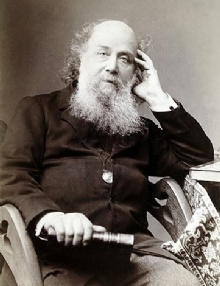
\includegraphics[height = 7cm]{j_sylvester.jpg}}
    \caption{J. Sylvester\\1814 – 1897}
  \end{minipage}
  \hfill
  \begin{minipage}[b]{0.31\textwidth}
    \captionsetup{labelformat=empty}
    \captionsetup{justification=centering}
    \framebox{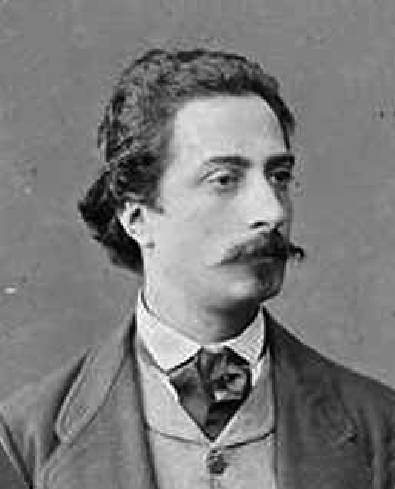
\includegraphics[height = 7cm]{e_beltrami.png}}
    \caption{E. Beltrami\\1835 - 1900}
  \end{minipage}
  \hfill
  \begin{minipage}[b]{0.31\textwidth}
    \captionsetup{labelformat=empty}
    \captionsetup{justification=centering}
    \framebox{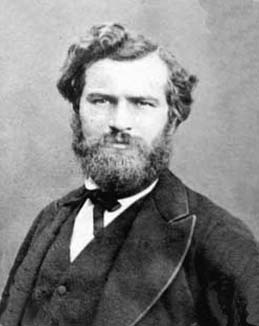
\includegraphics[height = 7cm]{c_jordan.jpeg}}
    \caption{C. Jordan\\1838 – 1922}
  \end{minipage}
\end{figure}
	\vfill % Whitespace between editor names and publisher logo

    
	%------------------------------------------------
	%	Publisher
	%------------------------------------------------
	
%	\plogo % Publisher logo
	
	\vspace{0.3\baselineskip} % Whitespace under the publisher logo
	
	Draft Version 0.935\\
    \today % current date
	
	%{\large publisher} % Publisher
    
    %%%% add ornament
	\cornerplus{63}{85}\thispagestyle{empty}
\end{titlepage}
%%%%%%%%%%%%% enf of title page


\pagestyle{fancy}
\fancyhf{}
\renewcommand{\sectionmark}[1]{\markright{\arabic{section}.\ #1}}
\fancyhead[l]{\nouppercase{\rightmark}}
\fancyfoot[c]{\thepage}
\renewcommand{\headrulewidth}{1pt}

%\maketitle

\newpage
\tableofcontents


\newpage


\section{Quadratic form}




\begin{shaded*}
\begin{definition}
A quadratic form is a polynomial in several variables where each term is of total degree two.  In other words it is linear combination of products of two variables (possibly repeated variables).
\end{definition}
\end{shaded*}

A quadratic form can neatly be written as a product of a matrix and two vectors. Example of quadratic forms are the following:

\[
\begin{gathered}
Q(x_{1}, x_{2}) = -x_{1}^{2} + 3x_{2}^{2},\\
\quad Q(x_{1}, x_{2}, x_{3})=5x_{1}^{2}-4x_{3}^{2}-x_{1}x_{2}+7x_{2}x_{3} \\
\quad Q(x_{1}, x_{2}, x_{3})=-x_{1}x_{2}+7x_{2}x_{3}+2x_{1}x_{3}
\end{gathered}
\]

A quadratic form can neatly be written as a product of a matrix that describes the polynomial coefficients with two vectors that store the free variables. For example, take the product

\[
\begin{bmatrix} x_{1} & x_2\end{bmatrix}
\begin{bmatrix} 1 & 2\\3 & 4\end{bmatrix}=
\begin{bmatrix}x_1 + 3x_2, & 2x_1 + 4x_2 \end{bmatrix}
\]

Now multiply with the column vector $\begin{bmatrix}x_1 & x_2 \end{bmatrix}^T$.

\[
\begin{split}
\begin{bmatrix}x_1 + 3x_2, & 2x_1 + 4x_2 \end{bmatrix}
\begin{bmatrix}x_1 \\ x_2 \end{bmatrix}=x_1^2+5x_{1}x_{2}+4x_2^2
\end{split}
\]

Note that the off-diagonal entries themselves do not affect the result, but their sum does. For example, $\begin{bmatrix} 1 & 2\\3 & 4\end{bmatrix}, \; \begin{bmatrix} 1 & 3\\2 & 4\end{bmatrix}, \; \begin{bmatrix} 1 & 2.5\\2.5 & 4\end{bmatrix}$ would all product the same polynomial. When we want to find which matrix produced the form, we will prefer the symmetric case.

\begin{corollary}
A quadratic form can be written as a function $Q: \mathbb{R}^{n}\rightarrow\mathbb{R}$ in the form
\begin{equation}
Q(\textbf{x})=\textbf{x}^{T}\textbf{Ax}
\end{equation}
, where $\textbf{A}$ an $n\times n$ real symmetric matrix.
\end{corollary}


As mentioned before, \textbf{x} is a column vector. Below we will discuss how we can quickly go from matrix \textbf{A} to its quadratic form polynomial Q(\textbf{x}) and vice versa. We assume, for ease, that \textbf{A} is $2\times2$.

\begin{equation*}
\textbf{A}=
\begin{bmatrix}
    a & b \\
    c & d
\end{bmatrix}
\end{equation*}
, with $b=c$ because \textbf{A} is symmetric.


\subsection{From matrix to quadratic form}
Let's find $Q(\textbf{x})=\textbf{x}^{T}\textbf{Ax}$ given $\textbf{x}=\begin{bmatrix}x_{1}\\x_{2}\end{bmatrix}$.
%% star turns off the counter
\begin{equation*}
  \begin{split}
  \textbf{x}^{T}\textbf{Ax}
  	&=
  	\begin{bmatrix}x_{1}&x_{2}\end{bmatrix}\begin{bmatrix}
    	a & b \\
    	c & d
	\end{bmatrix}
	\begin{bmatrix}x_{1}\\x_{2}\end{bmatrix}\\
    &=\begin{bmatrix}ax_{1}+cx_{2}&bx_{1}+dx_{2}\end{bmatrix} \begin{bmatrix}x_{1}\\x_{2}\end{bmatrix}\\
    &=ax_{1}^{2} + (b + c)x_{1}x_{2} + x_{2}^{2}
  	\end{split}
 \;
\end{equation*}
Therefore quadratic form is a linear combination of the squares $x_{1}^{2}, x_{2}^{2}$ and the cross-product term (terms in general) $x_{1}x_{2}. $Notice how for matrix \textbf{A} the diagonal elements ($i=j$) scale the squares and the off-diagonal ones ($i\neq j$) scale the cross-product term.
\begin{lemma}
Matrices \textbf{A} and $\hat{\textbf{A}}=\frac{\textbf{A}+\textbf{A}^{T}}{2}$ have the same quadratic form.
\end{lemma}
\begin{lemma}
Matrices \textbf{A} and $\textbf{A}^{T}$  have the same quadratic form, i.e.
\begin{equation}
Q(\textbf{x})=\textbf{x}^{T}\textbf{Ax}=\textbf{x}^{T}\textbf{A}^{T}\textbf{x}
\end{equation}
\begin{proof}
It is left to the reader. Verify it first for a $2\times2$ matrix.
\end{proof}
\end{lemma}

\begin{proof}
For matrix $\hat{\textbf{A}}$:
\begin{equation*}
  \begin{split}
  Q(\textbf{x})&=\textbf{x}^{T}\frac{\textbf{A}+\textbf{A}^{T}}{2}\textbf{x}\\
  &=\frac{1}{2}\Big(\textbf{x}^{T}\textbf{A}\textbf{x} + \textbf{x}^{T}\textbf{A}^{T}\textbf{x}\Big)\\
  &=\frac{1}{2}\Big(\textbf{x}^{T}\textbf{A}\textbf{x}+\textbf{x}^{T}\textbf{A}\textbf{x}\Big)=\textbf{x}^{T}\textbf{A}\textbf{x}
  \end{split}
\end{equation*}
\end{proof}
\begin{exmp}
If $\textbf{A}=
\begin{bmatrix}
3 & -1\\
-3 & 7
\end{bmatrix}$
, $\textbf{B}=
\begin{bmatrix}
3 & 0\\
0 & 7
\end{bmatrix}$
, $\textbf{C}=
\begin{bmatrix}
1 &		0	& 	-2\\
0 &		2	& 	7\\
-2&		7	& 	3
\end{bmatrix}$

find the quadratic form of 

\begin{multicols}{2}
  \begin{enumerate} [label=(\alph*)]
  \item $\B{A}$
  \item $\B{A}^{T}$
  \item $\frac{\B{A}+\B{A}^{T}}{2}$
  \item $\B{B}$
  \item $\B{C}$
\end{enumerate}
\end{multicols}

\end{exmp}
\TheSolution
  \begin{enumerate} [label=(\alph*)]
  \item $Q(\textbf{x})=3x_{1}^{2}+(-1-3)x_{1}x_{2}+7x_{2}^{2}=3x_{1}^{2}-4x_{1}x_{2}+7x_{2}^{2}$
  \item $Q(\textbf{x})=3x_{1}^{2}+(-3-1)x_{1}x_{2}+7x_{2}^{2}=3x_{1}^{2}-4x_{1}x_{2}+7x_{2}^{2}$
  \item $\frac{\textbf{A}+\textbf{A}^{T}}{2}=
    \frac{1}{2}\bigg(\begin{bmatrix}
    3 & -1\\
    -3 & 7
    \end{bmatrix}+
    \begin{bmatrix}
    3 & -3\\
    -1 & 7
    \end{bmatrix}\bigg)=
    \begin{bmatrix}
    3 & -2\\
    -2 & 7
    \end{bmatrix}$\\
    $\therefore Q(\textbf{x})=3x_{1}^{2}+(-2-2)x_{1}x_{2}+7x_{2}^{2}=3x_{1}^{2}-4x_{1}x_{2}+7x_{2}^{2}$
  \item $Q(\textbf{x})=3x_{1}^{2}+7x_{2}^{2}$
  \item $Q(\textbf{x})=x_{1}^{2}+2x_{1}^{2}+3x_{3}^{2}-4x_{1}x_{2}+14x_{2}x_{3}$
\end{enumerate}
\qedblack

\subsection{From quadratic form to matrix}
Suppose we are given that $Q(\textbf{x})=ax_{1}^{2} + ex_{1}x_{2} + dx_{2}^{2}$ for some $2\times2$ symmetric matrix \textbf{A}. We saw in the previous section that the symmetric matrix that yielded that product is:
\begin{equation*}
  \textbf{A}=
  \begin{bmatrix}
      a & \tfrac{e}{2} \\
      \tfrac{e}{2} & d
  \end{bmatrix}
\end{equation*}
In general, the coefficient of the cross-product $x_{i}x_{j}$ goes in entry $(i,j)$. When we want to recover matrix $\textbf{A}$ from $Q(\textbf{x})$, we want to recover the symmetric one and we'll see why.
\begin{exmp}
  If $Q(\textbf{x})=5x_{1}^{2}+3x_{2}^{2}+2x_{3}^{2}-x_{1}x_{2}+8x_{2}x_{3}$ is the quadratic form of some symmetric matrix $\textbf{A}$, find that matrix.
\end{exmp}   
   \begin{TheSolution}
    In the main diagonal we have $5,3,2$, For the cross-product entries we have 	$a_{12}=a_{21}=-1/2$, $a_{23}=a_{32}=4$, therefore:
        \begin{equation*}
            \textbf{A}=
              \begin{bmatrix}
              5&		-\tfrac{1}{2}&		0\\
              -\tfrac{1}{2}&	3&			4\\
              0&		4&			2
              \end{bmatrix}
        \end{equation*}
    \end{TheSolution}
\qedblack


\subsection{Change of variable in quadratic form}

\begin{shaded*}
\begin{definition}
If $x\in \mathbb{R}^{n}$, then a change of variable is an equation of the form
\begin{equation}\label{eq:3}
	\textbf{x}=\textbf{P}\textbf{y} \Longleftrightarrow \textbf{y}=\textbf{P}^{-1}\textbf{x}
\end{equation}
, where $\textbf{P}$ is an invertible matrix and $\textbf{y}\in \mathbb{R}^{n}$.
\end{definition}
\end{shaded*}

If we rewrite the quadratic form $Q(\textbf{x})=\textbf{x}^{T}\textbf{Ax}$, with the change of variable in \eqref{eq:3}, then we have
\begin{equation}
	Q(\textbf{x})=\textbf{y}^{T}\textbf{P}^{T}\textbf{APy}
\end{equation}
\faQuestionCircle \textit{ Why is this useful?}
\begin{addmargin}[2em]{0em}% 1em left, 2em right
  \textbf{A} is symmetric so if we choose the correct matrix $P$ we can diagonalise the product $\textbf{P}^{T}\textbf{AP}$, i.e. $\textbf{P}^{T}\textbf{AP}=\textbf{D}$, therefore we end up with a simpler quadratic form with no cross-product terms, only squares.
\end{addmargin}
\begin{equation}
	Q(\textbf{x})=\textbf{y}^{T}\textbf{D}\textbf{y}
\end{equation}
\faQuestionCircle \textit{ Which matrix should we choose to make the product diagonal?}
\begin{addmargin}[2em]{0em}% 1em left, 2em right
  We know that a symmetric matrix is diagonalised by its eigenvector matrix. Therefore $\textbf{P}$ must contain the eigenvector as columns.
\end{addmargin}
\begin{exmp}
  Make a change of variable to transform the quadratic form $Q(\textbf{x})=x_{1}^{2}-8x_{1}x_{2}+5x_{2}^{2}$ into a quadratic form with no cross-product terms \cite{lay}.
\end{exmp}

\begin{TheSolution}
Write Q(\textbf{x}) in matrix form:
\begin{equation*}
Q(\textbf{x}) = \textbf{x}^{T}\textbf{Ax},\quad \textbf{A}=\begin{bmatrix}
1&		-4\\
-4&		-5
\end{bmatrix}
\end{equation*}
Diagolonalise \textbf{A}, so begin by finding the eigenvalues from:
\begin{equation*}
\begin{gathered}
\textup{det}(\textbf{A}-\lambda \textbf{I}) = 0\Longrightarrow \\
\textup{det}\bigg( \begin{bmatrix}
1-\lambda	&	-4\\
-4			&	-5-\lambda\\
\end{bmatrix} \bigg)=0\Longrightarrow \\
(1-\lambda)(5+\lambda)+16=0\Longrightarrow \\
\lambda=3,\quad \lambda=-7
\end{gathered}
\end{equation*}
Find the eigenvector for $\lambda=3$.
\begin{equation*}
  \begin{gathered}
    \textbf{Au}=\lambda \textbf{u}\Longrightarrow \\
    \begin{bmatrix}
    1	&	-4\\
    -4			&	-5\\
    \end{bmatrix}\cdot \begin{bmatrix}x_{1}\\x_{2} \end{bmatrix}=3\begin{bmatrix}x_{1}\\x_{2} \end{bmatrix}\Longrightarrow \\
    \begin{bmatrix}x_{1}-4x_{2}\\-4x_{1}-5x_{2} \end{bmatrix}=3\begin{bmatrix}x_{1}\\x_{2}\end{bmatrix}\Longrightarrow \\
    \begin{cases}
    \quad \;x_{1}-4x_{2}=3x_{1}\\
    -4x_{1}-5x_{2}=3x_{2}
    \end{cases}\Longrightarrow \\
    x_{1}=-2,\quad x_{2}=1
  \end{gathered}
\end{equation*}
, i.e. $\textbf{u}=\begin{bmatrix}1&-2\end{bmatrix}^{T}$, or normalised $\hat{\textbf{u}}=\begin{bmatrix}1/\sqrt{5}&-2\sqrt{5}\end{bmatrix}^{T}$. Similarly we find the eigenvector for $\lambda=-7$ and we end up with the pairs:
\begin{equation*}
\lambda=3:\;\hat{\textbf{u}}=\frac{1}{\sqrt{5}}\begin{bmatrix}-2\\1\end{bmatrix},\quad
\lambda=-7:\;\hat{\textbf{u}}=\frac{1}{\sqrt{5}}\begin{bmatrix}1\\2\end{bmatrix}
\end{equation*}
Notice how the eigenvectors are \textit{perpendicular} as matrix $\textbf{A}$ is \textit{real and symmetric}. The diagonalised result contains the eigenvalues in decreasing order and the  matrix $\textbf{P}$ that diagonalises $\textbf{A}$ contains the corresponding eigenvectors.
\begin{equation*}
  \begin{gathered}
  \textbf{P}=\frac{1}{\sqrt{5}}\begin{bmatrix}
  -2	&	1\\
  1	&	2
  \end{bmatrix}, \quad
  \textbf{D}=\begin{bmatrix}
  3	&	0\\
  0	&	-7
  \end{bmatrix}\\
  \therefore
  \textbf{P}^{T}\textbf{AP}=\textbf{D}\Longrightarrow \\
  \textbf{A}=\textbf{PDP}^{T}
  \end{gathered}
\end{equation*}
Perform change of variable $\textbf{x}=\textbf{Py}$ in the quadratic product:
  \begin{equation*}
  \begin{split}
  Q(\textbf{x})&=\textbf{x}^{T}\textbf{Ax}=x_{1}^{2}-8x_{1}x_{2}-5x_{2}^{2}\eqtext{$x=Py$}\\
  &=\textbf{y}^{T}\textbf{Dy}=3y_{1}^{2}-7y_{2}^{2}
  \end{split}
  \end{equation*}
  \qedblack
\end{TheSolution}

\faQuestionCircle \textit{ So what is the process to diagonalise the quadratic form?}
\begin{addmargin}[2em]{0em}% 1em left, 2em right
  \begin{enumerate}
  \item Determine matrix $\textbf{A}$ from the quadratic form $\textbf{x}^{T}\textbf{Ax}$
  \item Calculate the orthogonal diagonalisation of $\textbf{A}$ (eigenvalue and eigenvector matrices $\textbf{D}, \textbf{P}$). Normalise the eigenvectors.
  \item Perform change of variable $\textbf{x}=\textbf{Py}$ in the quadratic form to obtain $\textbf{x}^{T}\textbf{Ax}=\textbf{y}^{T}\textbf{Dy}$.
  \end{enumerate}
\end{addmargin}



\section{Principal axes theorem}
In section 1, we concluded the following.

\begin{shaded*}
  \begin{theorem}
  Let $\textbf{A}$ be an $n\times n$ real symmetric matrix. Then there exists an orthogonal change of variable $\textbf{x}=\textbf{Py}$ that transforms the quadratic form $\textbf{x}^{T}\textbf{Ax}$ into a quadratic form $\textbf{y}^{T}\textbf{Ay}$ with no cross-product term.
  \end{theorem}
\end{shaded*}

\begin{shaded*}
\begin{definition}
The columns of $\textbf{P}$ are called \textit{principal axes}  of the quadratic form $\textbf{x}^{T}\textbf{Ax}$.
\end{definition}
\end{shaded*}

The vector $\textbf{y}$ is the coordinate vector of $\textbf{x}$ relative to the orthonormal basis of $\setRn$ given by these principal axes.
\subsection{A geometric view of the principal axes theorem}
If $\textbf{\B{A}}$ is $2\times 2$ and $Q(\B{x})=\B{x}^{T}\B{Ax}$ is its quadratic form, then if we expand it we can see that all points that satisfy
\begin{equation}\label{eq:2:1}
  \B{x}^{T}\B{Ax}=c
\end{equation}
correspond either to
\begin{itemize}
  \item an ellipse
  \item a hyperbola
  \item a parabola
  \item their degenerate cases, i.e. two intersecting lines or a single point.
\end{itemize}
Assuming $AC \neq 0$, the equation of an ellipse or hyperbola centred at the origin with axes $x'x, y'y$ (\textit{standard form}) is
\begin{equation}
	\begin{gathered}
		Ax^2+Cy^2=1\\
		\B{x}^{T}\begin{bmatrix}A & 0 \\ 0 & C \end{bmatrix}\B{x}=1
	\end{gathered}
\end{equation}
The equation of an ellipse or hyperbola rotated w.r.t. axes $x'x, y'y$ (non-standard form) is
\begin{equation}
	\begin{gathered}
	Ax^2+Bxy+Cy^2=1 \Longleftrightarrow \\
    \B{x}^{T}\begin{bmatrix}A & \tfrac{B}{2}\\\tfrac{B}{2} & C \end{bmatrix}\B{x}=1
	\end{gathered}
    \label{eq:ellipse_non_standard}
\end{equation}
Constants $A, B, C$ determine the type of conic (Appendix 1), if it is not degenerate, particularly if we define our characteristic matrix $\B{A}=\begin{bmatrix}A & \tfrac{B}{2}\\\tfrac{B}{2} & C\end{bmatrix}$:
\begin{itemize}
	\item If $B^2-4AC>0 \Longleftrightarrow det(\B{A})<0$, then $A,C$ have the same sign and it is an ellipse.
    \item If $B^2-4AC<0\Longleftrightarrow det(\B{A})>0$, then $A,C$ have opposite signs and is it a hyperbola.
    \item If $B^2-4AC=0\Longleftrightarrow det(\B{A})=0$, then either $A=0$ or $C=0$ have therefore the conic is a parabola.
\end{itemize}
Therefore the presence of the term $Bxy$ determines whether the locus is rotated w.r.t the standard axes or not. Why that is the case is explained in Appendix 1. Some examples illustrating what is mentioned are shown below.
\begin{figure}[H]
	\centering %centralizar a figura
	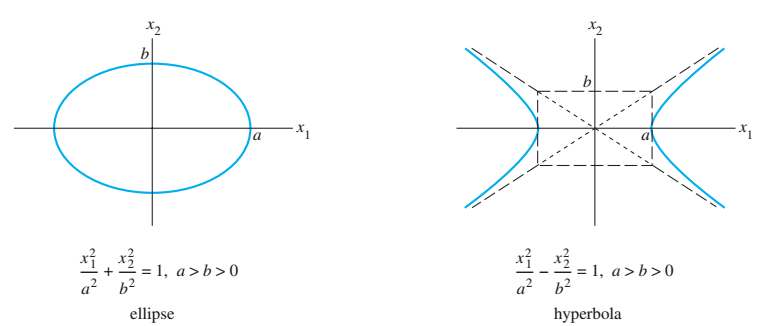
\includegraphics[height=5cm]{conics_standard.png}
    \caption{An ellipse and a hyperbola in standard position \cite{lay}}
    \label{fig:conics1}
\end{figure}
%Figure \ref{fig:conics1} shows a boat.
\begin{figure}[H]
	\centering %centralizar a figura
	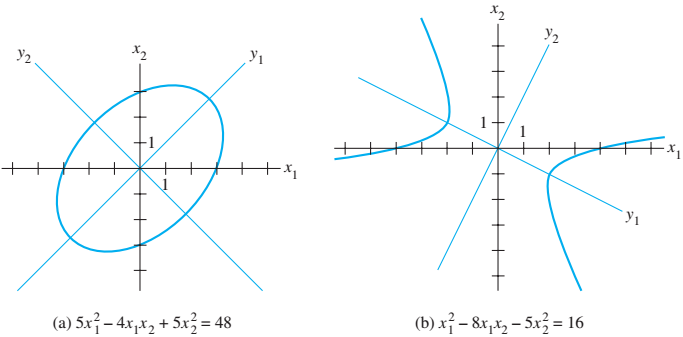
\includegraphics[height=5cm]{conics_standard2.png}
    \caption{An ellipse and a hyperbola in non-standard (rotated) position \cite{lay}}
    \label{fig:conics2}
\end{figure}
%%%%%%%%%%%%%%%%%%%%%%%%%%%%%%%%%%%%%%%%%
% fancy horizontal line
{\centering
{\Large \adforn{64}\rule{0.3\textwidth}{0.4pt}\hspace{0.2cm} \adforn{32}\adforn{7}\adforn{60} \hspace{0.2cm} \rule{0.3\textwidth }{0.4pt}\adforn{36}}\par
}
%%%%%%%%%%%%%%%%%%%%%%%%%%%%%%%%%%%%%%%%%
%\sectionlinetwo{black}{88}

Assuming that the quadratic form $Q(\B{x})=\B{x}^{T}\B{Ax}$ is an ellipse, we will show that making the substitution $\textbf{y}=\textbf{Px}$ has the effect of finding some new axes $y_{1}, y_{2}$, with respect to which the conic is in standard position. We will also express the length of the ellipse axes w.r.t. the eigenvalues of $A$.
\begin{corollary}
The primary and secondary axes point to the direction of the largest and smallest eigenvector respectively.
\end{corollary}
\begin{corollary}
The length of the primary and secondary axes of the standard ellipse given by the quadratic form $\B{x}^{T}\B{Ax}$ is $\sqrt{\lambda_{1}},\;\sqrt{\lambda_{2}}$ respectively, where $\lambda_{1}\leq\lambda_{2}$.
\end{corollary}
\begin{proof} \cite{stackexellipse1}
	We write matrix $\B{A}$ in its diagonalised form:
	\begin{equation*}
      A=\begin{bmatrix}\B{u}_1 & \B{u}_{2}\end{bmatrix}
          \begin{bmatrix}\lambda_{1} & 0\\0 & \lambda_{2}\end{bmatrix}
          \begin{bmatrix}\B{u}_1^{T} \\ \B{u}_{2}^{T}\end{bmatrix}
     \end{equation*}
	Then its quadratic form becomes:
    \begin{equation*}
    	\begin{split}
    	Q(\B{x})&=\B{x}^{T}\B{Ax}\\
        		&=\B{x}^{T}\begin{bmatrix}\B{u}_1 & \B{u}_{2}\end{bmatrix}
          \begin{bmatrix}\lambda_{1} & 0\\0 & \lambda_{2}\end{bmatrix}
          \begin{bmatrix}\B{u}_1^{T} \\ \B{u}_{2}^{T}\end{bmatrix}\B{x}\\
          	&=\lambda_{1}\B{x}^{T}\B{u}_{1}\B{u}_{1}^{T}\B{x}+\lambda_{2}\B{x}^{T}\B{u}_{2}\B{u}_{2}^{T}\B{x}
        \end{split}
    \end{equation*}

By setting the latter to a constant $c^2$, we can see what shape points $\B{x}=\begin{bmatrix}x_{1} & x_{2} \end{bmatrix}$ satisfy:
	\begin{equation*}
    	\begin{split}   
  \lambda_{1}\B{x}^{T}\B{u}_{1}\B{u}_{1}^{T}\B{x}+\lambda_{2}\B{x}^{T}\B{u}_{2}\B{u}_{2}^{T}\B{x}&=c \Longrightarrow \\
  \frac{(\B{u}_{1}\B{x})^{2}}{\Big(\frac{c}{\sqrt{\lambda_{1}}}\Big)^2}+\frac{(\B{u}_{2}\B{x})^{2}}{\Big(\frac{c}{\sqrt{\lambda_{2}}}\Big)^2}&=1 
        \end{split}
        \label{eq:ellipse} \tag{1}
    \end{equation*}
    Furthermore, \ref{eq:ellipse} says that the ellipse is centred w.r.t. the eigenvectors $\B{u}_1, \B{u}_{2}$, i.e. that they point to the ellipse axes.\\
    Another way to put this is as follows. Suppose a point on the ellipse is given as a linear combination of unit eigenvectors as basis - $\B{u}_1$ and $\B{u}_2$:
	\[
    \B{x}=y_{1}\B{u}_1+y_{2}\B{u}_2
    \label{eq:ellipse2} \tag{2}
    \]
    $y_{1}, y_{2}$ are the coordinates of $\B{x}$ w.r.t. the basis $\{\B{u}_{1},\B{u}_{2}\}$, therefore $y_{1}=\B{x}\cdot \B{u}_{1},y_{2}=\B{x}\cdot \B{u}_{2}$ so \eqref{eq:ellipse2} is rewritten as:
	\[    
      \frac{y_1^{2}}{\Big(\frac{c}{\sqrt{\lambda_{1}}}\Big)^2}+\frac{y_2^{2}}{\Big(\frac{c}{\sqrt{\lambda_{2}}}\Big)^2}=1 
      \tag{3} 
      \label{eq:ellipse3}
    \]

The points of the latter ellipse are centred w.r.t. the eigenvectors as basis vectors. If \eqref{eq:ellipse3} was not centred, there would be a $Bxy$ term in \eqref{eq:ellipse3} as we showed in \eqref{eq:ellipse_non_standard}.
 \end{proof} 
\begin{proof} \quad \\
    Therefore the length of the primary ($\alpha$) and secondary ($\beta$) semi axes is:
    \begin{equation}
    \alpha=\frac{c}{\sqrt(\lambda_{2})},\quad
    \beta=\frac{c}{\sqrt(\lambda_{1})},\quad\lambda_{1}\geq \lambda_{2}
    \label{eq:axes}
    \end{equation}
	Therefore the dominant eigenvalue defines the minor axis (steepest ascent) and the 	small eigenvalue defines the major axis.
\end{proof}

\begin{exmp}
Describe the curve (in terms of axes and rotation) $Q(\B{x})=8x_{1}^{2}-4x_{1}x_2+5x_{2}^{2},\quad \B{x}=\begin{bmatrix}x_1 & x_2 \end{bmatrix}^T$.
\end{exmp}
\begin{TheSolution}
$Q(\B{x})$ can be written as the quadratic form of matrix $\B{A}=\begin{bmatrix}8 &-2\\-2 & 5 \end{bmatrix}$.
\[
Q(\B{x})=\B{x}^{T}\begin{bmatrix}8 &-2\\-2 & 5 \end{bmatrix}\B{x}
\]
We want to remove the cross product hence find some new basis axes by making the substituion $\B{x}=\B{Py}$, where $\B{P}=\begin{bmatrix}\B{u}_1 & \B{u}_2\end{bmatrix}$, where $\B{u}_1, \B{u}_2$ are the eigenvectors of $\B{A}$.\\
Verify that
	\[
    \begin{gathered}
      \lambda_1=9:\space \space \B{u}_1=\begin{bmatrix}-2/\sqrt{5} & 1/\sqrt{5}\end{bmatrix}^T,\quad 	\lambda_2=4: \B{u}_2=\begin{bmatrix}1/\sqrt{5} & 2/\sqrt{5}\end{bmatrix}^T\\
      \therefore \B{P}=\frac{1}{\sqrt{5}}\begin{bmatrix}-2 & 1 \\1 & 2 \end{bmatrix},\quad \B{D}=\begin{bmatrix}\lambda_1 &0  \\ 0 & \lambda_2\end{bmatrix}=\begin{bmatrix}9 & 0\\0 &4 \end{bmatrix}
    \end{gathered}
    \]
    We've shown that $\B{P}$ diagonalises $\B{A}$, i.e. $P^{T}AP=D$ therefore using $\B{x}=\B{Py}$ we end up with
	\[   
    \begin{gathered}
    \B{y}^{T}\B{Dy}=1\Longrightarrow \\
    9y_1^{2}+4y_2^{2}=1 \Longrightarrow
    \end{gathered}
	\]
	\[
    	\frac{y_1^{2}}{\Big(\tfrac{1}{3}\Big)^2}+\frac{y_2^{2}}{\Big(\tfrac{1}{2}\Big)^2}=1
        \tag{\ding{168}}
        \label{eq:example_above}
    \]
    From  \eqref{eq:axes}, the length of the major and minor axes are respectively $\alpha=1/2,\space \beta=1/3$. Note that we have just verified that $\alpha=1/\sqrt{\lambda_2},\space \beta=1/\sqrt{\lambda_1},\space \lambda_1 \geq \lambda_2$.\\ 
    We finally want to know how the axes $y_{1},y_{2}$ of ellipse  \eqref{eq:example_above}, so essentially the eigenvectors of matrix $\bf{A}$ are rotated w.r.t. the standard axes. The angle of $u_{1}$ is $arctan(-0.5)=-26.56 mod\enspace 180\degree=153.44\degree$ and the angle of $u_{2}$ is $arctan(2)=63.43\degree$ ($mod\enspace 180$ because the angle is relative to the positive $x$ axis). The ellipse with its eigenvectors is shown below.
\begin{figure}[H]
	\centering %centralizar a figura
	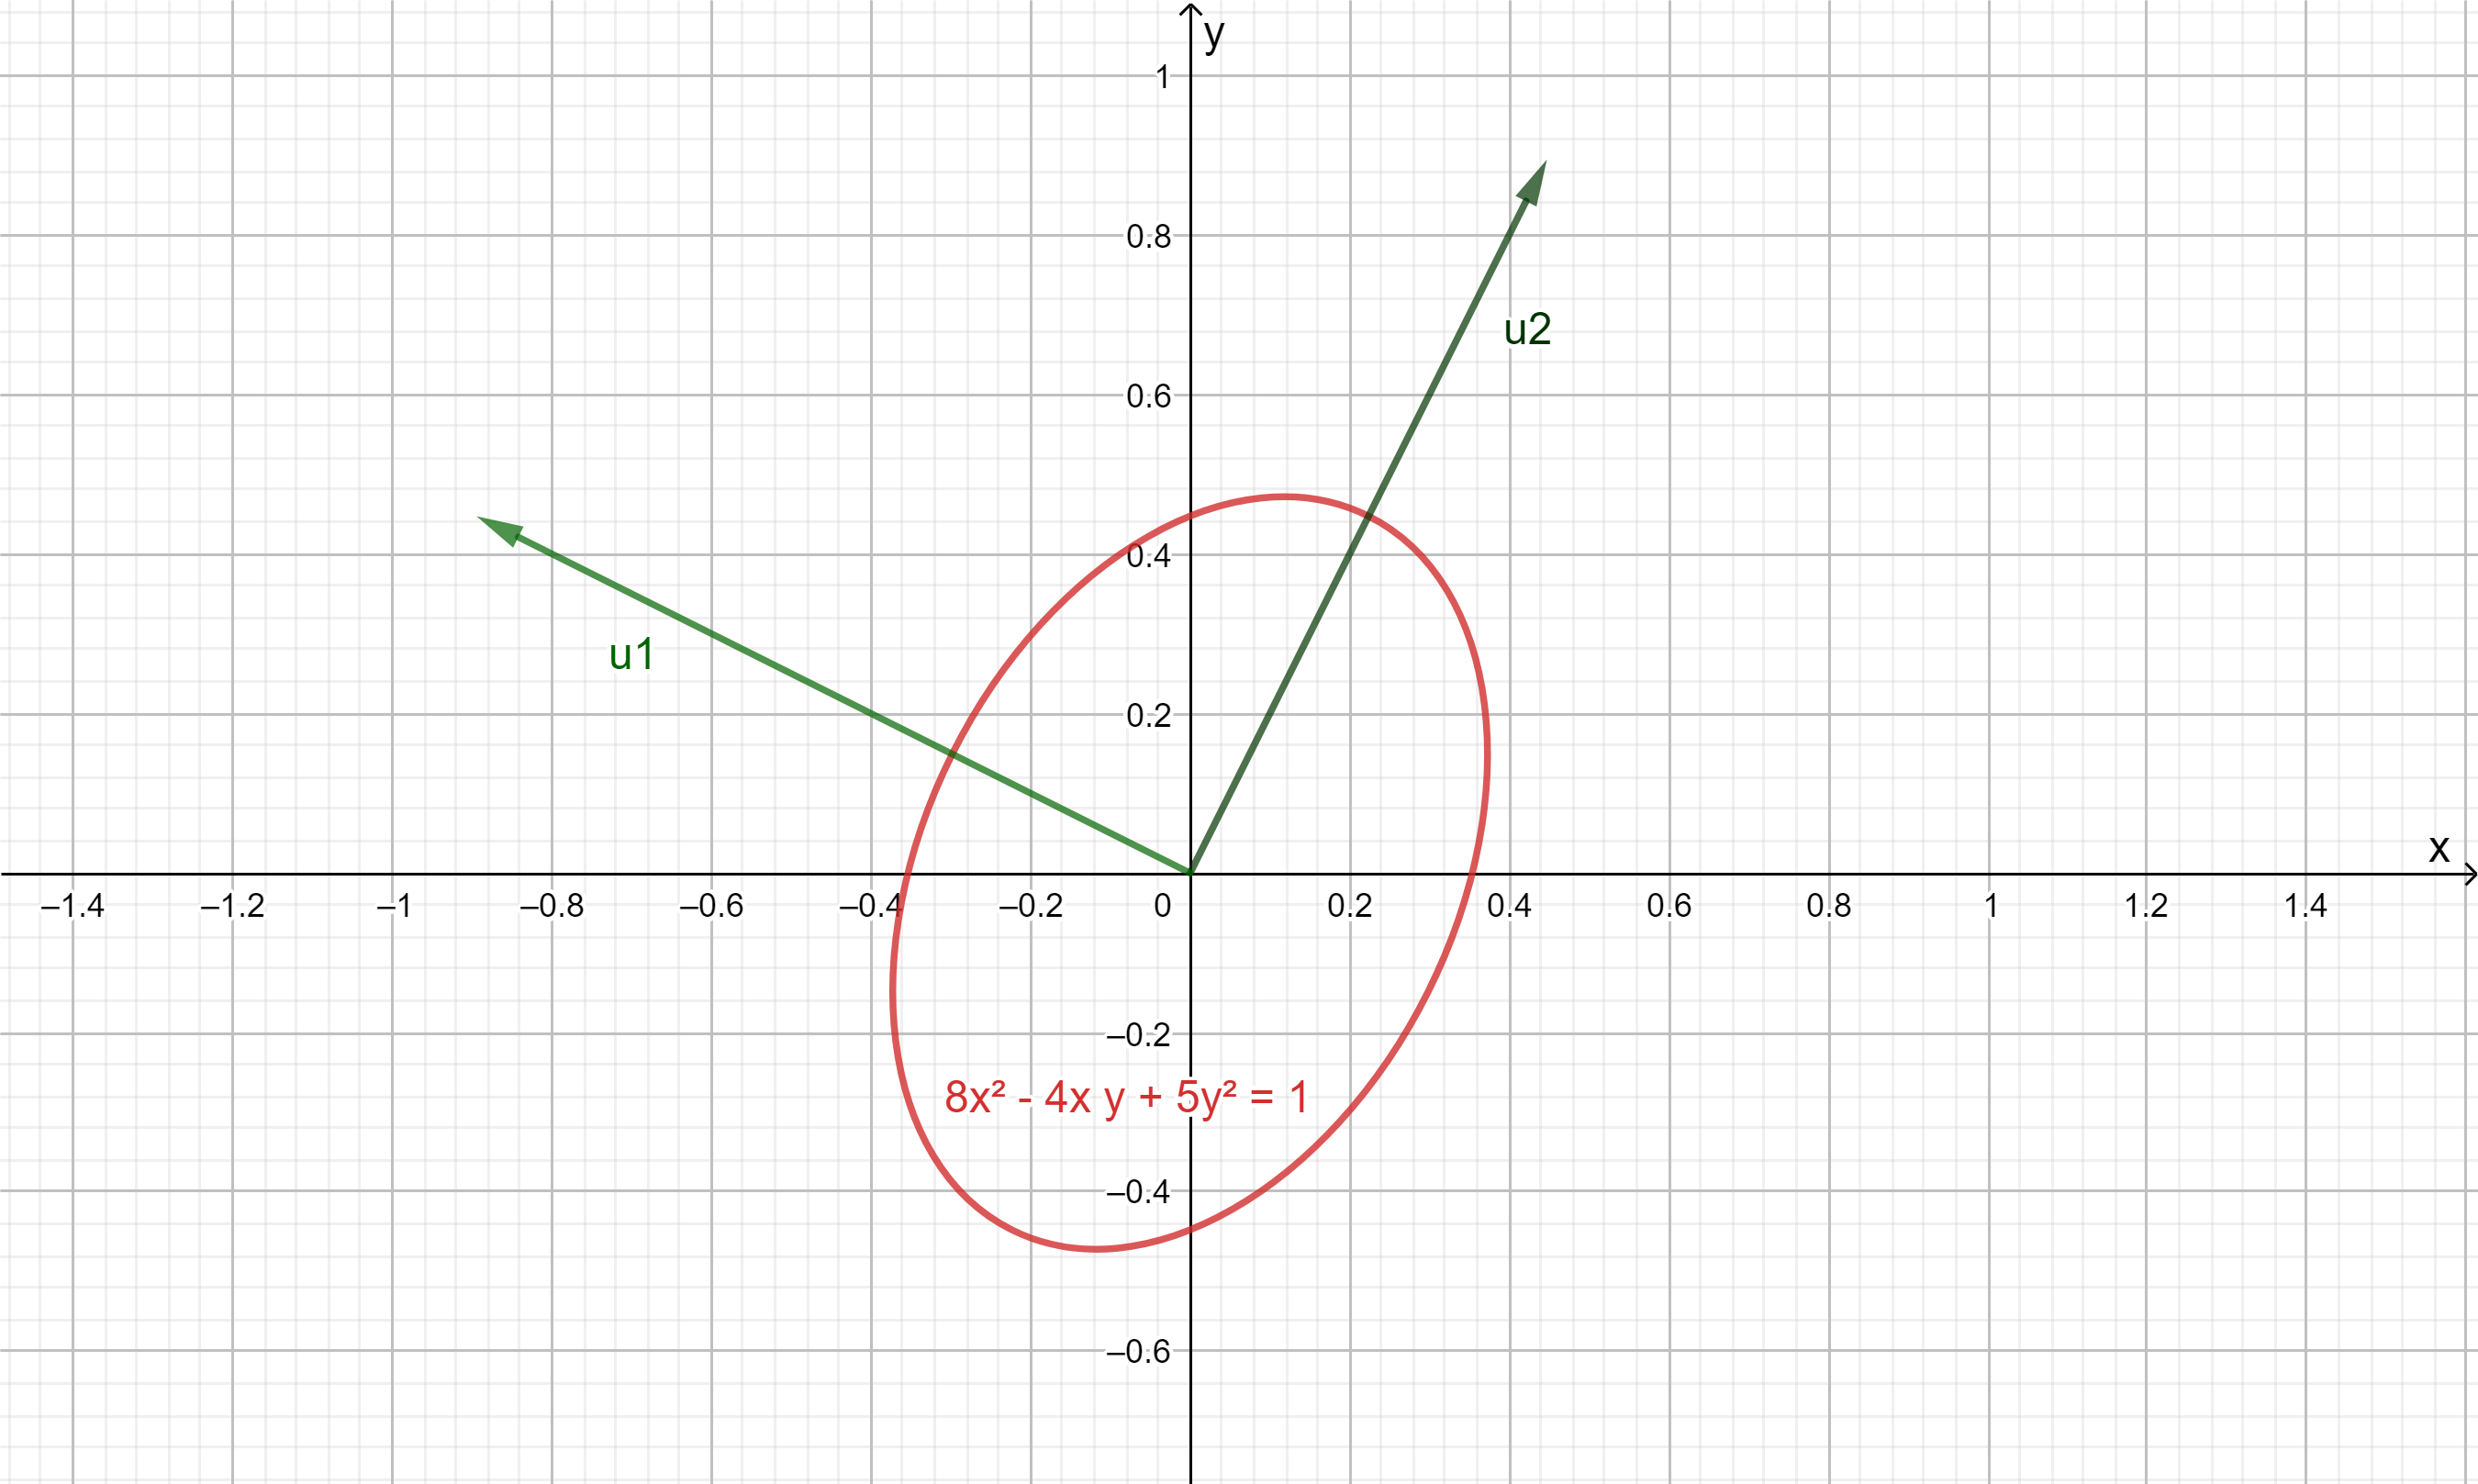
\includegraphics[height=5cm]{slant_ellipse_vecs.png}
    \caption{The ellipse given in the example. Notice how the unit eigenvectors point to the axes.}
    \label{fig:conics3}
\end{figure}
    \end{TheSolution}
\qedblack

  
  
  \section{Classifying quadratic surfaces}
  
As already mentioned, when $\bf{A}$ is a $n \times n$ matrix, the quadratic form $Q{(\bf{x})}=\bf{x}^{T}\bf{Ax}$ is a real-valued function $Q:\setRn \rightarrow \setR$. For example, if the domain is $\mathbb{R}^2$, then for points $(x_{1}, x_{2},z)$ for a certain value $z=Q(x_{1}, x_{2})$ correspond a horizontal cut of $z=Q(x_{1}, x_{2})$, therefore either to an ellipse or hyperbola or their degenerate cases \cite{lay}. As shown in the figures below, $z=Q(x_{1}, x_{2})$ describes
\begin{itemize}
  \item an elliptic paraboloid,
  \item or an ellipric hyperboloid
\end{itemize}
For the equations of those shapes, see Appendix 2. The important property is that an elliptic paraboloid is either convex or concave, therefore if its vertex is at $(0,0)$, it will be either non-negative or non-positive. Some examples are illustrated in Fig. \ref{fig:conics4}.
\begin{figure}[H]
	\centering %centralizar a figura
	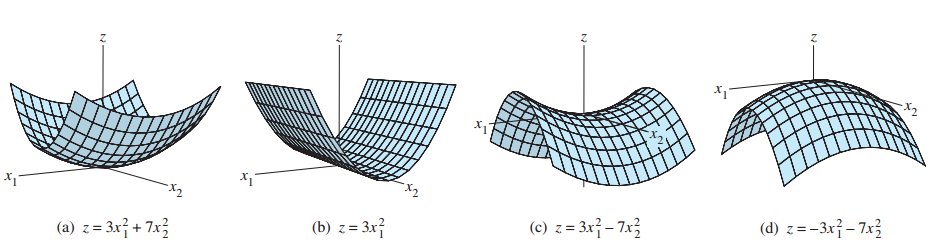
\includegraphics[height=4.25cm]{elliptic_oids.PNG}
    \caption{The ellipse given in the example. Notice how the unit eigenvectors point to the axes \cite{lay}.}
    \label{fig:conics_abcd}
\end{figure}
\begin{shaded*}
\begin{definition}
A quadratic form $Q(\B{x})=\B{x}^{T}\B{Ax}$ is
\begin{itemize}
  \item \emphasis{\textup{positive definite (PD)}} if $Q(\B{x})>0 \quad \forall \enspace \bf{x} \neq \bf{0}$.
  \item \emphasis{\textup{negative definite (ND)}} if $Q(\B{x})<0 \quad \forall \enspace \bf{x} \neq \bf{0}$.
  \item \emphasis{\textup{semi-positive (semi-negative) definite (SPD, SND)}} if $Q(\B{x})\geq 0\enspace (\leq 0) \quad \forall \enspace \bf{x} \neq \bf{0}$.
  \item indefinite if $Q(\B{x})$ assumes both positive and negative values.
\end{itemize}
\end{definition}
\end{shaded*}

\mycomment{Often, instead of saying that the quadratic form $\B{x}^T\B{Ax}$ is positive definite, we instead say that $\B{A}$ is positive definite. Both have the same meaning.
} % end comment
\begin{exmp}
Prove that if $\B{A}$ and $\B{B}$ are positive definite, then so is $\B{A}+\B{B}$.
\end{exmp}
\begin{TheSolution}
\[
\begin{gathered}
\B{x}^{T}\B{Ax} > 0 \hquad \forall \B{x} \in \setRn -\{\B{0}\}\\
\B{x}^{T}\B{Bx} > 0 \hquad \forall \B{x} \in \setRn -\{\B{0}\}\\
\therefore \B{x}^{T}(\B{A}+\B{B})\B{x} = \B{x}^{T}\B{Ax} + \B{x}^{T}\B{Bx} > 0
\end{gathered}
\]
\qedblack
\end{TheSolution}

Looking at Fig. \ref{fig:conics_abcd}, forms (a), (b) are semi-positive definite but (a) is described better at positive negative, as it is only $0$ at the origin. Positive definite and symmetric matrices are useful in a number of fields, such as statistics. We will prove how the following statements are equivalent \cite{chen_lec_notes}. 

\begin{enumerate} [label=(\alph*)]
  \item $\B{A}$ is positive definite and symmetric.
  \item All eigenvalues are positive.
  \item There exists factorisation of $\B{A}=\B{R}^{T}\B{R}$.
  \item All upper left determinants, including the main determinant itself, are positive.
  \item All pivots (without row exchanges) satisfy $d_{k}>0$.
\end{enumerate}

By upper left detetminants, we mean that if e.g. $\B{A}=\begin{bmatrix}2 & -1 & 0\\-1 & 2 & -1\\0 & -1 & 2 \end{bmatrix}$ then they are $2, \left| \begin{matrix}
   2 & -1  \\
   -1 & 2  \\
\end{matrix} \right|=3
, \left| \begin{matrix}2 & -1 & 0\\-1 & 2 & -1\\0 & -1 & 2 \end{matrix}\right|=4$.
  \begin{lemma}
  $(a) \Leftrightarrow (b)$ Let $\bf{A}$ be an $n \times n$ symmetric matrix. Then its quadratic form $\bf{x}^T\bf{Ax}$ is:
  \begin{itemize}
    \item positive definite iff the eigenvalues of $\bf{A}$ are all positive.
    \item negative definite iff the eigenvalues of $\bf{A}$ are all negative.
    \item indefinite iff $\bf{A}$ has both positive and negative eigenvalues.
  \end{itemize}
  \end{lemma}
  
\begin{proof} ($b \Rightarrow a$)\\
Assume all eigenvalues $\lambda_i, \; 1\leq i \leq n$ are positive. $\bf{A}$ is symmetric therefore by the Principal Axes theorem, there exists a change of variable $\bf{x}=\bf{Py}$ such that:
\[
Q(\bf{x})=\bf{x}^T\bf{Ax}=\bf{y}^T\bf{Dy}=\lambda_{1}y_{1}^2+\lambda_{2}y_{2}^2+\ldots+\lambda_{n}y_{n}^2
\]
So clearly $Q(\bf{x})>0$.

($a \Rightarrow b$)\\
Assume that $\B{A}$ is positive definite, i.e. $\B{x}^{T}\B{Ax}>0 \enspace \forall \enspace \B{x} \neq \B{0}$. If $\lambda$ is an eigenvalue and $\B{u}$ its eigenvector, then:
\[
\begin{gathered}
	\B{A}\B{u}=\lambda \B{u} \Longrightarrow \\
    \B{u}^{T}\B{A}\B{u} = \lambda \B{u}^{T}\B{u} \Longrightarrow \\
    \lambda = \frac{\B{u}^{T}\B{A}\B{u}}{\B{u}^{T}\B{u}}
\end{gathered}
\]
$\B{u}^{T}\B{A}\B{u}>0$ because of the hypothesis (zero eigenvectors are non meaningful) therefore $\lambda>0$.
\end{proof}

Positive definite matrices also admit a factorisation called Cholesky factorisation. How we obtain is explained in Appendix \ref{app:cholesky}.

\begin{lemma}
$(a \Leftrightarrow c)$ A symmetric and positive definite matrix $\B{A}$ admits a factorisation $\B{A}=\B{R}^{T}\B{R}$, where the columns of $\B{R}$ are linearly independent and vice versa.
\end{lemma}

\begin{proof}
\quad \\
Appendix \ref{app:cholesky}.
\end{proof}

\begin{lemma}
$(a)\Rightarrow (d)$ If $\B{A}$ is positive definite, then all upper left determinants are positive.
\end{lemma}
\begin{proof}\quad \\
Before we start, recall the following about the determinant of any matrix.
\begin{itemize}
\item Fact 1. The determinant of any matrix is the product of its eigenvalues.
\end{itemize}

Let $\B{A}$ be positive definite, $\bf{x} \in \setRn$, $k \leq n$, and $\B{x}_{k}$ the first $k$ entries of $\B{x}$. Then $\B{x}=\begin{bmatrix}\B{x}_{k} & \B{0} \end{bmatrix}$. $\B{A}$ is symmetric therefore partitioning its first $k \times k$ elements with the rest, we can write it as $\B{A}=\begin{bmatrix}\B{A}_{k} & \B{B}\\\B{B}^{T} & \B{C}  \end{bmatrix}$. We know that
\[
\begin{gathered}
\B{x}^{T}\B{A}\B{x}>0 \Longrightarrow \\
\begin{bmatrix}\B{x}_{k}^{T} & \B{0}^{T} \end{bmatrix} \begin{bmatrix}\B{A}_{k} & \B{B}\\\B{B}^{T} & \B{C}  \end{bmatrix} \begin{bmatrix}\B{x}_{k} & \B{0} \end{bmatrix}>0 \Longrightarrow \\
\B{x}_{k}^{T}\B{A}_{k}\B{x}_{k}>0 \quad \forall \quad \B{x}_{k}\neq \B{0}
\end{gathered}
\]

Therefore $((a)\Rightarrow (b))$ for all eigenvalues of $\B{A}$:

\[
\begin{gathered}
\lambda_{1},\lambda_{2},\ldots , \lambda_{n}>0 \Longrightarrow \\
\lambda_{1},\lambda_{2},\ldots , \lambda_{k}>0 \Longrightarrow \\
det(\B{A}_{k})=\lambda_{1}\lambda_{2}\ldots \lambda_{k}>0 \quad \forall \quad k \leq n
\end{gathered}
\]

\end{proof}

\begin{lemma}
$(a)\Rightarrow (e)$ All pivots $d_k$ of a real symmetric positive definite matrix satisfy $d_{k}>0$.
\end{lemma}
\begin{proof}
As shown in Appendix \ref{app:cholesky}, we can decompose $\B{A}$ as a product of a $\text{(lower triangular)} \times \text{(diagonal)} \times \text{(upper triangular)}$ matrices, i.e. "LDU":\\
\[
\B{A}=\B{LDU}
\]
$\B{L}, \B{U}$ are unit triangular and $\B{D}$ is diagonal containing the pivots. As in the previous lemma, partition $\B{A}$ as $\B{A}=\begin{bmatrix}\B{A}_{k} & \B{B}\\\B{B}^{T} & \B{C}  \end{bmatrix}$ and $\B{L}, \B{D}, \B{U}$ in the first $k \times k$ elements:

\[
\begin{gathered}
\begin{bmatrix}\B{A}_{k} & \B{B}\\\B{B}^{T} & \B{C}  \end{bmatrix}=
\begin{bmatrix}\B{L}_{k} & \B{0} \\ * & *\end{bmatrix}
\begin{bmatrix}\B{D}_{k} & \B{0} \\ \B{0} & * \end{bmatrix} 
\begin{bmatrix}\B{U}_{k} & * \\ * & \B{0}\end{bmatrix} \Longrightarrow \\
\B{A}_{k}=\B{L}_{k}\B{D}_{k}\B{U}_{k}
\end{gathered}
\]

Taking determinants above and because $\B{L}, \B{U}$ are triangular and have ones along the diagonal, while $\B{D}$ has the pivots:

\[
\begin{gathered}
\textup{det}(\B{A}_{k})=\textup{det}(\B{D}_{k})=d_{1}d_{2}\ldots d_{k} \\
\therefore d_{k} = \frac{\textup{det}(\B{A}_{k})}{\textup{det}(\B{A}_{k-1})}>0, \quad k=1,2,\ldots ,n
\end{gathered}
\]

\end{proof}

\begin{lemma}
$(e)\Rightarrow (a)$ If a real symmetric matrix $\B{A}$ has only positive pivots, then it is positive definite.
\end{lemma}

\begin{proof}
We have seen in App. \ref{app:cholesky} that when $\B{A}$ is symmetric, the LDU decompostion is:
\[
\B{A}=\B{LD}\B{L}^{T}
\]
, where $\B{D}$ stores the pivots. If $d_{ii}>0$, then
\[
\B{LD}\B{L}^{T}=\B{L}\B{D}^{1/2}\B{D}^{1/2}\B{L}^{T}=\B{R}^{T}\B{R}, \quad \B{R}=\B{D}^{1/2}\B{L}^{T}
\]
Therefore
\[
\B{x}^{T}\B{Ax}=\B{x}^{T}\B{R}^{T}\B{R}\B{x}=(\B{Rx})^{T}(\B{Rx})=\left\| \B{Rx} \right\|^{2}>0
\]
\end{proof} 

We have just proven the following important theorem. This is called \emphasis{Sylvester's theorem} and various other interesting proofs are found in \cite{article_csaki} and \cite{giorgi_definitiveness}.

\begin{shaded*}
\begin{theorem}
Each of the following tests is a necessary and sufficient condition for the real symmetric matrix $\B{A}$ to be positive definite \cite{chen_lec_notes}.
\begin{enumerate}
\item $\B{x}^{T}\B{Ax}>0 \quad \forall \B{x} \: \neq \B{0}$
\item All the eigenvalues of A satisfy $\lambda_i > 0$.
\item \B{A} admits a decomposition $\B{R}^{T}\B{R}$.
\item All the upper left submatrices $\B{A}_k$ have positive determinants
\item All the pivots (without row exchanges) satisfy $d_k > 0$
\end{enumerate}
\label{theorem:positive_def}
\end{theorem}
\end{shaded*}


\begin{exmp}
Prove that every positive definite matrix is invertible.
\end{exmp}
\begin{TheSolution}
We know
\[
\textup{det}(\B{A})=\lambda_{1}\lambda_{2}\ldots \lambda_n
\]
If $\B{A}$ wasn't invertible then:
\[
\exists \lambda_i:\ \textup{det}(\B{A})=0 \Leftrightarrow \lambda_i = 0, \hquad 1 \leq i \leq n
\]
That's contradicts the fact that because $\B{A}$ positive definite, then $\lambda_i>0$.
\end{TheSolution}

\begin{exmp}
Is $Q(\B{x})=3x_{1}^2+2x_{2}^2+x_{3}^2+4x_{1}x_{2}+4x_{2}x_{3}$ positive definite \cite{lay}?
\end{exmp}
\begin{TheSolution}
It may look like it is positive definite, however we need to find $\bf{A}$'s eigenvalues and write is as $\bf{y}^T\bf{Dy}$ first. The matrix $\bf{A}$ is:

	\[
    	\bf{A}=\begin{bmatrix}3 & 2 & 0\\ 2 & 2 & 2 \\ 0 & 2 & 1\end{bmatrix}
    \]
    We find $\lambda_{1} = 5, \enspace \lambda_{2} = 2, \enspace \lambda_{3} = -1$. Therefore $Q$ is indefinite.
\qedblack
\end{TheSolution}

\begin{exmp}
Determine whether matrix $\B{A}=
\begin{bmatrix}
2 & -1 & 0 \\ -1 & 2 & -1 \\0 & -1 & 2
\end{bmatrix}$
is positive definite \cite{chen_lec_notes}.
\end{exmp}

\begin{TheSolution}
First way:
\[
\begin{split}
\B{x}^{T}\B{Ax}&=2x_1^2+2x_2^2+2x_3^2-2x_{1}x_{2}-2x_{2}x_{3} \\
	&=2 \Big( x_1 - \frac{1}{2}x_2\Big)^2 + 
    \frac{3}{2}\Big( x_2 - \frac{2}{3}x_2\Big)^2 + 
    \frac{4}{3}x_3^2 > 0
\end{split}
\]
Second way:
\[
\lambda=2,\;2\pm \sqrt{2}
\]
Third way:
\[
\begin{split}
A_1 &= 2 \\
A_2&=\left| \begin{matrix} 2 & -1 \\-1 & 2\end{matrix}\right|=3 \\
A_3&=\left| \begin{matrix} 2 & -1 & 0\\-1 & 2 & -1\\ 0 & -1 & 2\end{matrix}\right|=4 \\
& \therefore A_1, \; A_2, \; A_3 > 0
\end{split}
\]
Fourth way:\\
The row reduced Echelon form of $\B{A}$ is $\B{I}_3$ ($3 \times 3$ unit matrix) so the pivots are $1,1,1$ - all positive. 


\end{TheSolution}

Finally, we have some similar criteria for a positive semi-definite matrix. Inverting the signs wouldn't work if we were to guess the criteria for a negative definite matrix but this will not be covered in this article.

\begin{exmp}
Let $\B{A}$ be an $n \times n$ invertible matrix. Show that if the quadratic form $\B{x}^{T}\B{Ax}$ is positive, then so is $\B{x}^{T}\B{A}^{-1}\B{x}$ and that the inverse is symmetric..
\end{exmp}
\begin{ASolution}
We know from Theorem \ref{theorem:positive_def} that if $\B{x}^{T}\B{Ax}>0 \hquad \B{x} \neq \B{0}$, then all its eigenvalues $\lambda_i$ are positive. For the eigenvalues of the inverse we know:
\[
\lambda_{-1,i}=\frac{1}{\lambda_i}>0
\]
From the same theorem, we have just proven what is required. Also:
\[
\big( \B{A}^{-1} \big)^{T}=\big( \B{A}^{T} \big)^{-1}=\B{A}^{-1} 
\]

\end{ASolution}
\begin{ASolution}
Define $\B{y}=\B{Ax}$ and take the quadratic form of $\B{A}^{-1}$:
\[
\begin{split}
\B{y}^{T}\B{A}^{-1}\B{y}&=
\B{x}^{T}\B{A}^{T}\B{A}^{-1}\B{A}\B{x}\\
&=\B{x}^{T}\B{A}^{T}\B{x}\\
&=\B{x}^{T}\B{A}\B{x}>0
\end{split}
\]
\end{ASolution}


\begin{shaded*}
\begin{theorem}
Each of the following tests is a necessary and sufficient condition for the real symmetric matrix $\B{A}$ to be positive semi-definite.
\begin{enumerate}
\item $\B{x}^{T}\B{Ax} \geq0 \quad \forall \B{x} \in \setRn$
\item All the eigenvalues of A satisfy $\lambda_i \geq 0$.
\item A admits a decomposition $\B{R}^{T}\B{R}$.
\item All the upper left submatrices $\B{A}_k$ have non-negative determinants
\item All the pivots (without row exchanges) satisfy $d_k \geq 0$
\end{enumerate}
\label{theorem:semi_pos_def}
\end{theorem}
\end{shaded*}

\begin{exmp}
\cite{lec_notes_zwick} Find the values of $b$ such that the following matrix is semi-positive definite.
\[
\begin{bmatrix}
2 & -1 & b\\-1 & 2 & -1\\b & -1 & 2
\end{bmatrix}
\]
\end{exmp}

\begin{TheSolution}
\[
\begin{gathered}
\left| \begin{matrix} 
2 & -1 & b\\-1 & 2 & -1\\b & -1 & 2
 \end{matrix} \right| =
6-2+b+b(1-2b) \geq0 \Leftrightarrow -1 \leq b \leq 2, \\
\left| \begin{matrix}  2 & -1 \\-1 & 2  \end{matrix}\right| >0, \\
2>0
\end{gathered}
\]
Therefore $-1 \leq b \leq 2$. \qedblack
\end{TheSolution}

For reference, we also have the following criterion for negative definitiveness. The proof is omitted, however various proofs are analysed at \cite{giorgi_definitiveness}.
\begin{shaded*}
\begin{theorem}
Each of the following tests is a  necessary and sufficient condition for the real symmetric matrix $\B{A}$ to be ND.
\begin{enumerate}
\item $\B{x}^{T}\B{Ax} \geq0 \quad \forall \B{x} \in \setRn$
\item All of the eigenvalues of $\B{A}$ satisfy $\lambda_i < 0$
\item All of its $k$-th order upper left principal minor shave sign $(-1)^k$.
\item All the pivots (without row exchanges) satisfy $d_k < 0$ 
\end{enumerate}
\label{theorem:negative_definite}
\end{theorem}
\end{shaded*}

\section{Constrained optimisation}

\subsection{Optimisation of quadratic form in the unit sphere}

Often we want to minimise or maximise a quadratic form subject to a constrained. One such contraint that allows us to easily study that is that the coordinate vector is unit, i.e. $\norm{\bf{x}}=1$, or equivalently

\begin{equation}
\norm{\B{x}}^2=\B{x}^{T}\B{x}=x_1^2+x_2^2+\ldots+x_n^2=1
\end{equation}

We will also see that when a quadratic form has no cross-product terms, it is easier to find its extrema for $\norm{\B{x}}=1$.

\begin{exmp}
Find the extrema of $Q(\B{x})=9x_1^2+4x_2^2+3x_3^2$ subject to $\norm{\B{x}}=1$ \cite{lay}.
\end{exmp}

\begin{TheSolution}
\[
\begin{split}
Q(\B{x}) &= 9x_1^2+4x_2^2+3x_3^2 \\
&\leq 9x_1^2+9x_2^2+9x_3^2\\
&= 9(x_1^2+x_2^2+x_3^2)\\
&= 9
\end{split}
\]
Notice that $Q(\B{x})=9$ for $\B{x}=(1,0,0)$. Therefore the maximum value is $9$. Similarly,
\[
\begin{split}
Q(\B{x}) &= 9x_1^2+4x_2^2+3x_3^2 \\
&\geq 3x_1^2+3x_2^2+3x_3^2\\
&= 3(x_1^2+x_2^2+x_3^2)\\
&= 3
\end{split}
\]
, with $Q(\B{x})=3$ for $\B{x}=(0,0,1)$, therefore the minimum is $3$. \qedblack
\end{TheSolution}

Let's consider matrix $\B{A}=\begin{bmatrix}3 & 0\\0 & 7\end{bmatrix}$ and its quadratic form $Q(\B{x})=\B{x}^{T}\B{Ax}, \hquad \B{x} \in \setR ^2$. We want to visualise the extrema of $Q(\B{x})$ given the constraint $\norm{\B{x}}=1$.\\
By setting $z=\B{x}^{T}\B{Ax}=3x_1^2+7x_2^2$, it is clear that the surface $z(x_1,x_2)$ is a positive paraboloid with minimum of 0 at $(0,0)$. The condition $\norm{\B{x}}=1$ adds the contraint that the points for which $z(x_1,x_2)$ is minimised or maximised must lie on the cylinder along the $z$ axis with radius of $1$. Note also that $z(x_1,x_2)$ grows fastest in height along axis $x_2$ and slowest along $x_1$.\\

\begin{figure}[H]
	\centering %centralizar a figura
	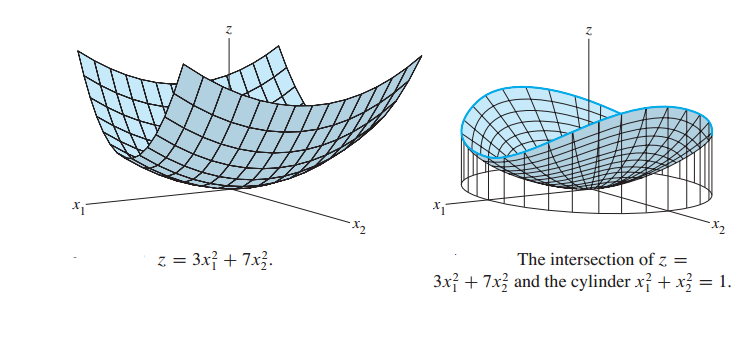
\includegraphics[height=4.25cm]{opt_01.PNG}
    \caption{The surface and its intersection with the cylinder $\norm{\B{x}}=1$, representing the constraint \cite{lay}.}
    \label{fig:conics4}
\end{figure}

The highest value of 7 given $\norm{\B{x}}=1$ occurs at the eigenvector $\B{u}_1=\begin{bmatrix}0 & 1 \end{bmatrix}$ and it's equal to the eigenvalue $\lambda_1=7$. The minimum value of 3 occurs at the eigenvector $\B{u}_2=\begin{bmatrix}1 & 0 \end{bmatrix}$ and it's equal to the eigenvalue $\lambda_2=3$.\\

\begin{lemma}
If $\B{A}$ is a symmetric matrix, all possible values for $\B{x}^{T}\B{Ax}$, given $\norm{\B{x}}=1$, are real.
\end{lemma}
\begin{proof}
\TODO[both in one proof]
\end{proof}

\begin{lemma}
Denote the right and left endpoints of this interval by $m$ and $M$ respectively, i.e.

\begin{equation}
m=min\{\B{x}^{T}\B{Ax}, \hquad \norm{\B{x}}=1 \}, \hquad M=max\{\B{x}^{T}\B{Ax}, \hquad \norm{\B{x}}=1 \}
\label{eq:max_min}
\end{equation}

If $\lambda$ is an eigenvalue of $\B{A}$, then $m\leq \lambda \leq M$.
\end{lemma}
\begin{proof} \quad \\
Let  $\B{u}$ be a unit eigenvector of $\B{A}$ for the eigenvalue $\lambda$ and $m,M$ the minimum and maximum of the quadratic form, then:
\[
\begin{gathered}
\B{u}^{T}\B{Ax}=\B{u}^{T}\lambda \B{u}=\lambda \norm{\B{u}}^2=\lambda \\
\therefore m \leq \lambda \leq M
\end{gathered}
\] 
\end{proof}
The next theorem says that there exists eigenvalues of $\B{A}$ $m$ and $M$ are themselves.

\begin{shaded*}
\begin{theorem}
Let $\B{A}$ be a symmetric matrix and $m, M$ be defined as in  \eqref{eq:max_min}. Then $M$ is equal to the greatest eigenvalue $\lambda_1$ of $\B{A}$ and $m$ to the smallest eigenvalue $\lambda_n$. $\B{x}^{T}\B{Ax}=M$ when $\B{x}=\B{u}_1$ and  $\B{x}^{T}\B{Ax}=m$ when $\B{x}=\B{u}_n$, where $\B{u}_1, \hquad \B{u}_n$ are the unit eigenvectors corresponding to $\lambda_1, \lambda_n$ \cite{lay}.
\end{theorem}
\end{shaded*}

\begin{proof}
\quad \\
Before we start, we use the following facts:

\begin{enumerate}
\item If $\B{A}$ is orthogonally diagonalised as $\B{PD}\B{P}^{-1}$, then by setting $\B{x}=\B{Py}$ the cross-product is removed from the quadtatic form:

\[
\B{x}^{T}\B{Ax}=\B{y}^{T}\B{Ay}
\tag{\ding{171}}
\label{eq:opt_proof_quad}
\]

\item $\B{x}^T\B{Ax}$ and $\B{y}^T\B{Dy}$ assume the same range of values. The transformation $\B{x}=\B{Py}$ only rotates $\B{x}$ without changing its magnitude, as $\B{P}$ is orthonormal, i.e. $\B{P}^T\B{P}=\B{I}$.

\[
\begin{gathered}
\norm{\B{x}}^2= \norm{\B{Py}}^2 = 1\Longrightarrow \\
 (\B{Py})^T(\B{Py}) = \B{y}^{T}\B{P}^{T}\B{P}\B{y}=1 \Longrightarrow\\
\norm{\B{y}}=1
\end{gathered}
\tag{\ding{171}\ding{171}}
\label{eq:opt_proof_quad}
\]

\item The eigenvalues of a real and symmetric matrix are non-negative.
\end{enumerate}

To simplify the notation, assume $\B{A}$ is a $3 \times 3$ matrix with eigenvalues $\lambda_1 \geq \lambda_2 \geq \lambda_3 \geq 0$ and arrange the corresponding eigenvectors in $\B{P}$ in the same order so that:
\[
\B{P}=\begin{bmatrix}\B{u}_1 & \B{u}_2 & \B{u}_3 \end{bmatrix}, \hquad
\B{D}=\begin{bmatrix}\lambda_1 & & \\ & \lambda_2 & \\ & & \lambda_3\end{bmatrix}
\]

For any vector $\B{y} \in \setR ^ 3$:

\[
\begin{gathered}
\begin{aligned}
\lambda_1 y_1^2 &= \lambda_1 y_1^2 \\
\lambda_2 y_2^2 &= \lambda_1 y_2^2 \\
\lambda_3 y_3^2 &= \lambda_1 y_3^2 \Longrightarrow \\
\end{aligned}\\
\begin{aligned}
\B{y}^T\B{Dy} &= \lambda_1 y_1^2+ \lambda_2 y_2^2 + \lambda_3 y_3^2 \\
& \leq \lambda_1 y_1^2+ \lambda_1 y_2^2 + \lambda_1 y_3^2 \\
& = \lambda_1 (y_1^2 + y_2^2 + y_3^2) \\
& = \lambda_1 \norm{\B{y}}^2 = \lambda_1
\end{aligned}
\end{gathered}
\]

Therefore $\lambda_1 \geq M$. Also $\B{e}_1^T\B{D}\B{e}_1=\lambda_1$ so the maximum of $\B{y}^{T}\B{Ay}$ is $\lambda_1$ attained for $\B{y}=\B{e}_1$. Similarly, $\lambda_3$ is the minimum of $\B{y}^{T}\B{Ay}$ for $\B{y}=\B{e}_3$. \\
From Fact 2 (\TODO[re-do the numbering above]) we know the two quadratic forms assume the same range, therefore when one is maximum the other is maximum too. Hence $M=\lambda_1=\B{e}_1^{T}\B{De}_1=\B{u}_1^{T}\B{Au}_1$, so the maximum is attained when $\B{x}=\B{Pe}_1=\B{u}_1$. $m=\lambda_3=\B{e}_3^{T}\B{De}_3=\B{u}_3^{T}\B{Au}_3$ attained when $\B{x}=\B{Pe}_3=\B{u}_3$.
\end{proof}


\begin{exmp}
Let $\B{A}=\begin{bmatrix} 3 & 2 & 1\\2 & 3& 1\\1& 1& 4\end{bmatrix}$. Find the maximum value of the quadratic form $\B{x}^T\B{Ax}$ subject to $\norm{\B{x}}=1$ \cite{lay}.
\end{exmp}

\begin{TheSolution}
We find the greatest eigenvalue to be $\lambda=6$. \\
The constrained maximum of $\B{x}^T\B{Ax}$ is attained when $\B{x}$ is the unit eigenvector corresponding to $\lambda=6$. Solving $\B{A}-6\B{I}=0$ we find $\B{x}=\begin{bmatrix}1 & 1 & 1 \end{bmatrix}^T$ therefore $\B{u}=1/\sqrt{3}\begin{bmatrix}1 & 1 & 1 \end{bmatrix}^T$. \qedblack
\end{TheSolution}

Below we maximise the quadratic form with some additional constraints.

\begin{shaded*}
\begin{theorem}
\cite{lay}Let $\lambda_1,\lambda_2,\ldots, \lambda_n$, $\B{u}_1,\B{u}_2,\ldots, \B{u}_n$ be the eigenvalues and eigenvectors of a symmetric matrix $\B{A}$. Then the maximum value of $\B{x}^T\B{Ax}$ subject to the constraints
\[
\B{x}^T\B{u}_1=0, \quad \norm{\B{x}}=1
\]
is the second gretaest eigenvalue $\lambda_2$ and it is attained when $\B{x}$ is the unit eigenvector $\B{u}_2$ corresponding to $\lambda_2$.
\end{theorem}
\end{shaded*}

As a generalisation, we have the following.

\begin{shaded*}
\begin{theorem}
\cite{lay}~Let$\B{A}$ be a symmetric $n \times n$ matrix with  an orthogonal diagonalisation $\B{A}=\B{PD}\B{P}^{-1}$, where the entries on the diagonal are arranged such that $\lambda_1 \geq \lambda_2  \ldots, \lambda_n $ and the columns of $\B{P}$ are the corresponding eigenvectors $\B{u}_1,\B{u}_2, \ldots , \B{u}_n$. Then for $k=1,2,\ldots,n$ the maximum value of $\B{x}^{T}\B{Ax}$ subject to
\[
\B{x}^T\B{u}_1=0, \B{x}^T\B{u}_2=0,\ldots, \B{x}^T\B{u}_n=0,\quad \norm{\B{x}}=1
\]
is the eigenvalue $\lambda_k$, and this maximum is attained for $\B{x}=\B{u}_k$.
\end{theorem}
\end{shaded*}


\begin{exmp}
Maximise $q(x,y)=xy$ given the constraint $4x^2+9y^2 \leq 36$ \cite{lay}.
\end{exmp}
Note: Each point $(x,y)$ that satisfies the constraint is called \emphasis{feasible solution}. The curve $4x^2+9y^2 = 36$ is called \emphasis{constraint curve}. The set of points for which $4x^2+9y^2 = const$ is called \emphasis{indifference curve}.

\begin{TheSolution}
In our problem, we do not have a "unit sphere constraint" for the input free variables so we need to create one. We have\\
\[
\begin{gathered}
4x^2+9y^2 \leq 36 \Longrightarrow \\
% [...] for text bellow xArrow
\Big(\frac{x}{3}\Big)^2 + \Big(\frac{y}{2}\Big)^2 \leq 1 \xRightarrow[y'=\tfrac{y}{2}]{x'=\tfrac{x}{3}}\\
\big(x' \big)^2 + \big(y' \big)^2 \leq 1 
\end{gathered}
\]

The function we want to minimise becomes

\[
q(x',y')=6x'y'
\]

It can now be written in quadratic form given the "unit sphere constraint" therefore its maximum can be found.

\[
q(x',y')=6x'y'=\B{x}\begin{bmatrix}0 & 3\\0 & 3 \end{bmatrix}\B{x}
\]
For matrix $\B{A}$, $\lambda=3,-3$ with eigenvectors $\B{x}=\begin{bmatrix}1/\sqrt{2} & 1/\sqrt{2} \end{bmatrix}^T, \hquad \begin{bmatrix}-1/\sqrt{2} & 1/\sqrt{2} \end{bmatrix}^T$
Therefore the maximum value of $3$ is attained at $(x',y')=(\tfrac{1}{\sqrt{2}},\tfrac{1}{\sqrt{2}})$ therefore for $(x,y)=(\tfrac{3}{\sqrt{2}},\tfrac{2}{\sqrt{2}})$.
\end{TheSolution}
%%%%%%%%%%%%%%%%%%%%%%%%%%%%%%%%%%%%%%%%%
% fancy horizontal line
{\centering
{\Large \adforn{64}\rule{0.3\textwidth}{0.4pt}\hspace{0.2cm} \adforn{32}\adforn{7}\adforn{60} \hspace{0.2cm} \rule{0.3\textwidth }{0.4pt}\adforn{36}}\par
}
%%%%%%%%%%%%%%%%%%%%%%%%%%%%%%%%%%%%%%%%%


\subsection{(Optional) Optimisation of general 2nd order form}



\subsubsection{Unbounded quadric problem (part 1)}


In this section, we want to minimise an \emphasis{objective function} of the form
\begin{equation}
f(\B{x})=\frac{1}{2}\B{x}^T\B{H}\B{x}+\B{c}^T\B{x}+c_0
\label{eq:general_2nd_order}
\end{equation}
In order to minimise the function in \eqref{eq:general_2nd_order}, we will show that \B{H} has to be semi positive definite. Assume that \B{H} is negative definite, i.e. there exists $\B{d} \in \setRn$ such that $\B{d}^T\B{H}\B{d}<0$, then:

\[
f(t\B{x})=\frac{1}{2}t^2\B{d}^T\B{H}\B{d}+t\B{c}^T\B{d}+c_0 \rightarrow -\infty \quad \text{as} \quad t \rightarrow \infty
\]

Therefore \B{H} has to be positive definite and according to Appendix \ref{app:cholesky}, it admits an "LDU" factorisation, i.e. $\B{H}=\B{L}^T\B{DL}$ with $\B{L}$ lower triangular, where $\B{D}=diag(d_1,d_2,\ldots,d_n)$, with $d_i \geq 0 \hquad \forall \hquad 1\leq i \leq n$ according to Theorem \ref{theorem:semi_pos_def}. As shown in \cite{lec_notes_kth}, The problem becomes
\[
\begin{split}
&\text{minimise }\frac{1}{2}\B{x}^T\B{H}\B{x}+\B{c}^T\B{x}+c_0\\
&=\text{minimise }\frac{1}{2}\B{x}^T\B{L}^T\B{DL}\B{x}+\B{c}^T(\B{L}^T)^{-1}\B{L}^T\B{x}+c_0 \\
&=\text{minimise } \sum\limits_{k=1}^{n}{\frac{1}{2}{{d}_{k}}y_{k}^{2}+{{{\tilde{c}}}_{k}}{{y}_{k}}+{{c}_{0}}} \\
&=c_0 + \sum\limits_{k=1}^{n}{\text{minimise } \frac{1}{2}{{d}_{k}}y_{k}^{2}+{{{\tilde{c}}}_{k}}{{y}_{k}}} \\
\end{split}
\]
We have introduced the new coordinates 
\begin{equation}
y=\B{L}^T\B{x}, \quad \tilde{c}=\B{L}^{-1}\B{c}
\end{equation}
The minimisation can now be decoupled to $n$ independent scalar quadratic problems.


\subsubsection{Scalar quadratic optimization without constraints}

The scalar quadratic form
\[
p(x)=ax^2+2bx+c
\]
(2 factor because it's generated by a symmetric matrix) has a minimum only if $a>0$. By differentiating we have:
\[
\begin{split}
p'(x)&=2ax+2b \\ 
p'(x) & \npsym 0 \Leftrightarrow x \npsym -\frac{b}{a} \\
p'(x) & = 0 \Leftrightarrow x = -\frac{b}{a}
\end{split}
\]
Therefore $p(x)$ is strictly decreasing for $x<-\tfrac{b}{a}$ and strictly increasing for $x>-\tfrac{b}{a}$, which means that the minimum occurs at 
\begin{equation}
x^{\star}=-\frac{b}{a}, \text{where } p(x^{\star})=c-\frac{b^2}{a}
\label{eq:scalar_min}
\end{equation}


\subsubsection{Unbounded quadratic problem (part 2)}

Applying  \eqref{eq:scalar_min} to solve our minimisation sub-problems separately, we find for each $\hat{y_i}$ that $\hat{\B{y}}_i=-\tfrac{\tilde{c}_k}{d_k}$, given the semi-positive definitiveness condition $d_k \geq 0$. So for a minimiser $\hat{\B{y}}=\begin{bmatrix}\hat{y}_1 & \hat{y}_2 & \ldots & \hat{y}_n\end{bmatrix}^T$  we have the following lemma \cite{lec_notes_kth}. 
 
\begin{lemma}
The objective function 
\begin{equation}
f(\B{x})=\frac{1}{2}\B{x}^T\B{H}\B{x}+\B{c}^T\B{x}+c_0
\label{eq:quadratic_full_vector}
\end{equation}
is minimised when
\[
g(\B{x})=\sum\limits_{k=1}^{n}{\frac{1}{2}{{d}_{k}}y_{k}^{2}+{{{\tilde{c}}}_{k}}{{y}_{k}}}
\]
is minimised, where $\B{x}=\B{LD}\B{L}^T, \quad \B{y}=\B{L}^T\B{x}, \quad \tilde{\B{c}}=\B{L}^{-1}\B{c}$. Vector $\hat{\B{y}}$ is a minimiser of $g(x)$ if:
\begin{enumerate}
\item  $d_i \geq 0 \hquad \forall \hquad 1\leq i \leq n \Leftrightarrow$ $\B{H}$ is semi positive definite.
\item $d_k \hat{y}_k=-\tilde{c}_k \quad \quad \quad \Leftrightarrow \B{DL}^T\hat{\B{x}}=-\B{L}^{-1}\B{c} \Leftrightarrow \B{LD}\B{L}^T\hat{\B{x}}=-\B{c} $
\end{enumerate}
$\hat{x}$ is simply the respective $\hat{\B{x}}$ vector for which $\B{y}$ is a (unique) minimiser. Using LDU factorisation and for the global minimiser $\B{x}^{\star}$, constraint (2) can be simplified to: 
\label{lemma:unconstrained_min}
\end{lemma}
\begin{equation}
\B{H}\B{x}^{\star}=-\B{c} \quad \xLeftrightarrow{\text{\B{H} PD}} \quad \B{x}^{\star}=-\B{H}^{-1}\B{c} \label{eq:glob_min_x}
\end{equation}

The second form holds \emphasis{only if} $\B{H}$ is positive definite. Then the minimum value of $f(\B{x})$ is
\[
f(-\B{H}^{-1}\B{c})=-\frac{1}{2}\B{c}^{T}\B{H}^{-1}\B{c}+c_0
\]

Note that to remember  \eqref{eq:glob_min_x}, we can compare the objective function $f(\B{x})$ in  \eqref{eq:quadratic_full_vector} with the scalar quadratic form $f(x)=ax^2+2bx+c$ and the minimiser in \eqref{eq:glob_min_x} with the scalr one $ax=-b$.\\
Furthermore, inverting any of the conditions in Lemma \ref{lemma:unconstrained_min}, we can find when $f(x)=\frac{1}{2}\B{x}^T\B{H}\B{x}+\B{c}^T\B{x}+c_0$ is unbounded from below \cite{lec_notes_kth}.

\begin{lemma}
$f(x)=\frac{1}{2}\B{x}^T\B{H}\B{x}+\B{c}^T\B{x}+c_0$ is unbounded from below if:
\begin{enumerate}
\item  Some $d_k < 0 \hquad \Leftrightarrow$ $\B{H}$ is not semi-positive definite.
\item There exists $k$ such that one of the equations 
\[
d_k \hat{y}_k=-\tilde{c}_k
\]
do not have a solution, i.e. $d_k=0$ and $\tilde{c}_k \neq 0$
$d_k \hat{y}_k=-\tilde{c}_k\Leftrightarrow \B{DL}^T\hat{\B{x}}=-\B{L}^{-1}\B{c}$
ivalently, the last condition says that the system $\B{H}\hat{\B{x}}=-\B{c}$ does not have a solution.
\end{enumerate}
\end{lemma}

The above arguments can be formalised as the following theorem

\begin{shaded*}
\begin{theorem}
Let $f(x)=\frac{1}{2}\B{x}^T\B{H}\B{x}+\B{c}^T\B{x}+c_0$. Then $\B{x}^{\star}$ is a minimiser if
\begin{enumerate}
\item $\B{H}$ is semi positive definite.
\item $\B{H}{\B{x}^{\star}}=-\B{c}$
\end{enumerate}
\end{theorem}
\end{shaded*}
Note: The condition that $\B{H}{\B{x}^{\star}}=-\B{c}$ has a solution equivalently tells us that $\B{c} \in \mathcal{R}(\B{H})$, where $\mathcal{R}$ denotes the range, also known as column space.

\begin{exmp}
Minimise the quadratic form $Q(x_1,x_2)=4x_1^2-2x_1x_2+3x_2^2+3x_1-2x_2+1, \quad x_1,x_2 \in \setR$ \cite{lec_notes_olver}.
\end{exmp}
\begin{TheSolution}
Write $Q(x_1,x_2)$ in the general quadratic form as in  \eqref{eq:general_2nd_order}.
\[
Q(x_1,x_2)=\frac{1}{2}\begin{bmatrix}x_1 & x_2 \end{bmatrix}
\begin{bmatrix}8 & -2 \\-2 & 6 \end{bmatrix}
\begin{bmatrix}x_1 \\ x_2 \end{bmatrix} +
\begin{bmatrix} x_1 & x_2\end{bmatrix}
\begin{bmatrix} 3 \\ -2\end{bmatrix}
+ 1
\]
Therefore $\B{H}=\begin{bmatrix}8 & -2 \\-2 & 6 \end{bmatrix}$, $\B{c}=\begin{bmatrix} -3 \\ 2\end{bmatrix}$ (don't forget to factor out the $\tfrac{1}{2}$. Then we have showed that the minimiser vector $\B{x}^{\star}$ is found by solving the system
\[
\begin{bmatrix}8 & -2 \\-2 & 6 \end{bmatrix}
\begin{bmatrix}x_1 \\ x_2 \end{bmatrix} = 
\begin{bmatrix} -3 \\ 2\end{bmatrix}
\]
$\B{H}$ is positive definite thus invertible therefore $f(\B{x})$ really has a minimum, obtained by Gaussian elimination at 
\[
\B{x}^{\star}=\begin{bmatrix}-\frac{7}{22} \\ \frac{5}{22} \end{bmatrix}\approx
\begin{bmatrix}-.318 \\ .227 \end{bmatrix}
\]
with value $Q(\B{x}^{\star})=Q(-\frac{7}{22},\frac{5}{22}) \approx .295$ \qedblack.
\end{TheSolution}

\subsubsection{Unconstrained optimisation using analytic methods; the Hessian matrix}
We will show how we can minimise the function in the last example using analytical methods. Algebraic and analytic methods are connected by the Hessian matrix $\B{H}$, which appears in both. We can often use analytical methods to verify our results. First a reminder.

\begin{shaded*}
\begin{definition}
The \emphasis{gradient} or "del" of a multi variable differentiable function $f(x_1,x_2,\ldots,x_n)$ is a vector operator denoted as $\boldsymbol{\nabla }f$ or simply $\nabla f$. In 3D cartesian coordinates, the gradient is given by the vector
\begin{equation}
\nabla f = \frac{\partial f}{\partial x}\mathbf{i}+\frac{\partial f}{\partial y}\mathbf{j}+\frac{\partial f}{\partial z}\mathbf{k}
\end{equation}

\end{definition}
\end{shaded*}
Alternatively, in more compact notation and denoting $\partial _x f:=\tfrac{\partial f}{\partial x}$, it is given by $\nabla f=\left(\partial_x f,\partial_y f,\partial_z f\right)$ or in matrix notation $\nabla f=\begin{bmatrix} \partial_x f & \partial_y f & \partial_z f\end{bmatrix}^T$. Some properties of the gradient are presented in \ref{app:app_gradient}.\\
The gradient is useful because it lets us compute the Taylor series of a multi variable function, which in terms lets us derive an optimisation property of the Hessian matrix.\\
The following definitions help us establish a criterion for multi variable function optimisation.
\begin{shaded*}
\begin{definition}
A differentiable multi variable function $f:\setRn \rightarrow \setR$ exhibits a \emphasis{critical point} at $\B{x}^{\star} = (x_1,x_2,\ldots,x_n)$ if:
\begin{equation}
\nabla f(\B{x}^{\star}) = 0 \Leftrightarrow f_{x1}(\B{x}^{\star})=f_{x2}(\B{x}^{\star})=\ldots=f_{xn}(\B{x}^{\star})=0
\end{equation}
\end{definition}
\end{shaded*}
\begin{shaded*}
\begin{definition}
Let $f:\setRn \rightarrow \setR$ be a function whose second partial derivatives exist  and are continuous over the domain of the function. Its Hessian matrix $\B{H}$ is a $n \times n$ matrix defined as
\\ \quad % equation was going off the margin
\begin{equation}
\B{H}=
\begin{bmatrix}
   \frac{{{\partial }^{2}}f}{\partial {{x}_{1}}^{2}} & \frac{{{\partial }^{2}}f}{\partial {{x}_{1}}\partial {{x}_{2}}} & \cdots  & \frac{{{\partial }^{2}}f}{\partial {{x}_{1}}\partial {{x}_{n}}}  \\
   \frac{{{\partial }^{2}}f}{\partial {{x}_{2}}\partial {{x}_{1}}} & \frac{{{\partial }^{2}}f}{\partial {{x}_{2}}^{2}} & \cdots  & \frac{{{\partial }^{2}}f}{\partial {{x}_{2}}\partial {{x}_{n}}}  \\
   \vdots  & \vdots  & \ddots  & \vdots   \\
   \frac{{{\partial }^{2}}f}{\partial {{x}_{n}}\partial {{x}_{1}}} & \frac{{{\partial }^{2}}f}{\partial {{x}_{n}}\partial {{x}_{2}}} & \cdots  & \frac{{{\partial }^{2}}f}{\partial {{x}_{n}}^{2}}  \\
\end{bmatrix} 
\label{eq:hessian_def}
\end{equation}
\end{definition}
\end{shaded*}
Hessian in \eqref{eq:hessian_def} can tell us whether the ctitical point is a local maximum, minumum, or saddle point. For a 2-variable function, we have proven the following theorem in App. \ref{app:taylor_multivar} using Taylor series. A more detailed proof is found in \cite{book_beck}.
\begin{shaded*}
\begin{theorem}
Let $f(x,y)$ be a twice differentiable function, and let $(x_0,y_0)$ be a critical point for $f$, i.e. $\nabla f(x_0,y_0)=0$.
\begin{enumerate}
\item If $\B{H}_f(x_0,y_0)$ is positive definite, then $x_0,y_0$ is a local minimum for $f$.
\item If $\B{H}_f(x_0,y_0)$ is negative definite, then $x_0,y_0$ is a local maximum for $f$.
\item If $\B{H}_f(x_0,y_0)$ is indefinite, then $x_0,y_0$ is a saddle point for $f$.
\item If $\B{H}_f(x_0,y_0)=0$, then the second derivative test doesn't tell us anything and we need a higher order approximation.
\end{enumerate}
\label{theorem:crit_point_hessian}
\end{theorem}
\end{shaded*}
We can use Theorem \ref{theorem:crit_point_hessian} to solve the example in the previous section using analytic ways.
\begin{exmp}
Minimise the quadratic form $Q(x,y)=4x^2-2xy+3y^2+3x-2y+1, \quad x,y \in \setR$.
\end{exmp}
\begin{TheSolution}
Compute the partial derivatives, denoting $f_x := \tfrac{\partial f}{\partial x}, f_y := \tfrac{\partial f}{\partial y}$: \\
\TODO[align them vertically centered in a nice way]
\begin{align*}
&f_x = 8x - 2y + 3 & & & & f_y = -2x + 6y - 2 \\
&f_{xx} = 8 > 0 & & f_{yy} = 6 & &  f_{xy} = -2
\end{align*}
The critical point is determined by solving:
\begin{align*}
&f_{x} = 0 & & \textup{and} & & f_{y} = 0 & \Leftrightarrow \\
&8x - 2y + 3 = 0 & & \textup{and} & & -2x + 6y - 2  = 0 & \Leftrightarrow \\
& x = -\frac{7}{22} & & & & y = \frac{5}{22}
\end{align*}
Therefore the only critical point is that $(x_0,y_0) = ( -\tfrac{7}{22}, \tfrac{5}{22}) $. Evaluate the Hessian at it.
\[
\B{H}_f (x_0,y_0) = \begin{bmatrix}8 & -2 \\-2 & 6 \end{bmatrix}
\]
For matrix $\B{H}_f (x_0,y_0)$, we have $8>0$ and $\textup{det}(\B{H}_f) (x_0,y_0) = 44 > 0$ therefore it is positive definite. Alternatively, we could find the eigenvalues $\lambda_1 = 7+\sqrt{5}>0, \lambda_2 = 7 - \sqrt{5} > 0$ so again, according to Theorem \ref{theorem:positive_def} it is positive definite. The definitiveness combined with $f_{xx}(x_0,y_0) > 0$ guarantee that $(x_0,y_0)$ is a local minimum and as it's the only minimum, it's also global. \qedblack
\end{TheSolution}

\begin{exmp} Find and classify the critical points of the function $f(x,y)=3x^2y + y^3 -3x^2 - 3y^2 + 1$ \cite{pauls_notes_minmax}.
\end{exmp}
\begin{TheSolution}
Find the partial derivatives:
\TODO[align them vertically centered in a nice way]
\begin{align*}
&f_x = 6xy - 6x & & & & f_y = 3x^2 + 3y^2 - 6y \\
&f_{xx} = 6y-6 > 0 & & f_{yy} = 6y-6 & &  f_{xy} = 6x
\end{align*}
Both $f_{xx},f_{yy}$ are continuous. By solving $f_x=0,\ f_y=0$ we find that the critical points are $(0,0),(0,2),(1,1),(-1,1)$. Compute the Hessian:
\[
\B{H}_f = \begin{bmatrix} 6y-6 &  6x\\6x & 6y-6\end{bmatrix}
\]
For each critical point, we have:
\begin{enumerate}
\item At $(0,0)$, $\textup{det}(\B{H}_f)=36 > 0$ and $f_{xx}=-6 <0$ therefore local maximum.
\item At $(0,2)$, $\textup{det}(\B{H}_f)=36 > 0$ and $f_{xx}=6 > 0$ therefore local minimum.
\item At $(1,1)$, $\textup{det}(\B{H}_f)=-36 < 0$ therefore saddle point.
\item At $(-1,1)$, $\textup{det}(\B{H}_f)=-36 < 0$ therefore saddle point.
\end{enumerate}
\qedblack

\end{TheSolution}


%%%%%%%%%%%%%%%%%%%%%%%%%%%%%%%%%%%%%%%%%
% fancy horizontal line
{\centering
{\Large \adforn{64}\rule{0.3\textwidth}{0.4pt}\hspace{0.2cm} \adforn{32}\adforn{7}\adforn{60} \hspace{0.2cm} \rule{0.3\textwidth }{0.4pt}\adforn{36}}\par
}
%%%%%%%%%%%%%%%%%%%%%%%%%%%%%%%%%%%%%%%%%


\subsubsection{Constrained optimisation with linear constraint}

We now focus on the following problem.\\
\begin{equation}
\begin{gathered}
\textup{Minimise } f(\B{x})=\frac{1}{2}\B{x}^{T}\B{H}\B{x}+\B{c}^{T}\B{x}+c_0 \\
\textup{s. t. } \B{Ax}=\B{b},\\
\textup{where } \B{H}=\B{H}^T \in \setR ^{n \times n}, \hquad \B{A} \in \setR ^{m \times n}, \hquad \B{b} \in \setR ^{m}, \hquad \textup{and } c_0 \in \setR .
\end{gathered}
\label{eq:constr_opt_problem}
\end{equation}
The set $\mathcal{F}$ of all vectors $\B{x} \in \setRn$ that satisfy the constraint $\B{Ax}=\B{b}$ is called \emphasis{feasible solution}. Therefore $\mathcal{F}=\{\B{x} \in \setRn\; : \: \B{Ax}=\B{b}\}$.

\begin{itemize}
\item If the system $\B{Ax}=\B{b}$ has no solution, i.e. $\B{b} \notin \mathcal{R}(\B{A})$, then $\mathcal{F}=\emptyset$ therefore there is no contrained minimisation proble.
\item If the system $\B{Ax}=\B{b}$ has exactly one solution, then this solution is also the uniqueo ptimal solution to the problem \eqref{eq:constr_opt_problem}, since there is no other feasible solution which is better.
\item The only non-trivial case is when $\B{Ax}=\B{b}$ has multiple different solution, which is the case when $\B{A}$ has more columns than rows, i.e. $m>n$ and the columns are lin. independent, therefore span $\setR^m$. Then $\B{b} \in \mathcal{R}(\B{A})$ and $\mathcal{N}(\B{A}) \neq \emptyset$. Also $\mathcal{R}(\B{A})$ spans $\setR ^m \Rightarrow dim( \mathcal{R}(\B{A}))=m$ and $dim(\mathcal{N}(\B{A}))=n-m$. 
\end{itemize}

So for the rest of this section we assume $n>m$, which means that:
\begin{equation}
\B{b} \in \mathcal{R}(\B{A}), \quad \mathcal{N}(\B{A}) \neq \emptyset
\end{equation}

We also have the following lemma about a feasible solution $\bar{\B{x}}$ of the system and any other solution $\B{x}$.

\begin{lemma}
If $\bar{\B{x}} $ is a feasible solution of $\B{Ax}=\B{b}$ then
\[
\begin{gathered}
\B{x} \in \mathcal{F} \Longleftrightarrow 
\bar{\B{x}} - \B{x} \in \mathcal{N}(\B{A})
\end{gathered}
\]
\end{lemma}
\begin{proof}\quad \\
$(\Rightarrow)$:

\[
\begin{gathered}
\bar{\B{x}} \in \mathcal{F} \Rightarrow \B{A}\bar{\B{x}} = \B{b} \quad
\B{x} \in \mathcal{F} \Rightarrow \B{A}\B{x} = \B{b} \\
\therefore \B{A}(\bar{\B{x}} - \B{x}) = \B{b} - \B{b} = \B{0} \\
\therefore \bar{\B{x}} - \B{x} \in \fancyN(\B{A})
\end{gathered}
\]

$(\Leftarrow)$:\\
If $\bar{\B{x}}$ is a feasible solution and $ \bar{\B{x}} - \B{x} \in \mathcal{N}(\B{A})$, we want to show that $\B{x}$ is also a feasible solution.
\[
\begin{gathered}
\bar{\B{x}} - \B{x} \in \mathcal{\B{A}} \Rightarrow \B{A}(\B{x} - \bar{\B{x}}) = 0\\
\therefore \B{A}\B{x} = \B{A}(\B{x} - \bar{\B{x}}  + \bar{\B{x}} ) = 
\B{A}(\B{x} - \bar{\B{x}})+\B{A}\bar{\B{x}} = \B{b}
\end{gathered}
\]
\end{proof}

Let $k$  be the dimension of $\mathcal{N}(\B{A})$ and $\B{z}_1,\B{z}_2,\ldots, \B{z}_k$ be the coefficient vectors that are its basis. 
\[
\B{Z}=\begin{bmatrix} \B{z}_1 & \ldots & \B{z}_k \end{bmatrix}
\]
Let $\B{v}$ be the $k \times 1$ coordinate vector. Then $\bar{\B{x}} - \B{x} \in \mathcal{N}(\B{A}) $ iff $\bar{\B{x}} - \B{x} = \B{vZ}$ for some arbitary $\B{v} \in \setR^k$~\cite{lec_notes_wang},~\cite{book_bunch}, therefore for any feasible solution we get the representation:
\[
\B{x} \in \mathcal{F} \textup{ iff } \B{x} = \bar{\B{x}} + \B{Zv} \textup{ for some } \B{v} \in \setR^k
\]
Since $\B{z}_1,\B{z}_2,\ldots, \B{z}_k$ are linearly independent, it follows that for every $\B{x} \in \mathcal{F}$ there is a unique $\B{v} \in \setR^ k$.

Therefore we want to minimise $f( \bar{\B{x}} + \B{Zv})$. The following two lemmas show how $f( \bar{\B{x}} + \B{Zv})$ can be expanded.

\begin{lemma}
If $t \in \setR, \hquad \B{d} \in \setRn$, then for the quadratic function in  \eqref{eq:quadratic_full_vector} we have~\cite{lec_notes_sasane}
\begin{equation}
\nonumber
f(\B{x}+t\B{d}) = f(\B{x}) + t(\B{Hx}+\B{c})^T \B{d} + \frac{1}{2}t^2\B{d}^T\B{Hd} \quad \forall \B{x} \in \setRn
\end{equation}
\label{lemma:quad_form_of_sum}
\end{lemma}

\begin{proof}
\[
\begin{split}
f(\B{x}+t\B{d}) &= \frac{1}{2}(\B{x}+t\B{d})^T \B{H}(\B{x}+t\B{d}) + \B{c}^T (\B{x}+t\B{d})  + c_0 \\
&= \frac{1}{2}\Big(\B{x}^T\B{Hx} +t\B{d}^T\B{Hx} + t\B{x}^T\B{Hd} +t^2\B{d}^T\B{Hd} \Big) + \B{c}^T\B{x} + t\B{c}^T\B{d} + c_0 \\
&= \Big(\frac{1}{2}\B{x}^T\B{Hx}+\B{c}^T\B{x} + c_0\Big) + t\Big(\frac{1}{2}\B{d}^T\B{Hx} + \frac{1}{2}\B{x}^T \B{Hd} + \B{c}^T \B{d} \Big)+\frac{1}{2}t^2\B{d}^T\B{Hd}\\
&=f(\B{x}) + t(\B{Hx} + \B{c})^T\B{d} + \frac{1}{2} t^2 \B{d}^T\B{Hd}
\end{split}
\]
\end{proof}

\begin{lemma}
From Lemma \ref{lemma:quad_form_of_sum} for $t=1, \hquad \B{d}=\B{y} - \B{x}$ we obtain~\cite{lec_notes_sasane}
\[
f(\B{y}) = f(\B{x}) + (\B{Hx} + \B{c})^T \B{d} + \frac{1}{2}t^2\B{d}^T \B{Hd}
\]
\label{lemma:quad_form_of_diff}
\end{lemma}

Now we can compute $f( \bar{\B{x}} + \B{Zv})$ using Lemma \ref{lemma:quad_form_of_diff} for $d=1, \hquad \B{d}=\B{Zv}$:
\[
\begin{split}
f( \bar{\B{x}}) + \B{Zv}&=f( \bar{\B{x}}) + (\B{H}\bar{\B{x}} + \B{c})^T\B{Zv} + \frac{1}{2}(\B{Zv})^T \B{H}(\B{Zv}) \\
&= f( \bar{\B{x}}) + (\B{Z}^T(\B{H}\bar{\B{x}} + \B{c}))^T\B{v} + \frac{1}{2}\B{v}^T(\B{Z}^T\B{HZ})\B{v}
\end{split}
\]

Therefore we have transformed the problem to an unconstrained one, namely

\begin{equation}
\begin{gathered}
\textup{minimise } f( \bar{\B{x}}) + (\B{Z}^T(\B{H}\bar{\B{x}} + \B{c}))^T\B{v} + \frac{1}{2}\B{v}^T(\B{Z}^T\B{HZ})\B{v}\\
\textup{s.t. } \B{v} \in \setR ^ k
\end{gathered}
\label{eq:cost_to_unconst_opt_problem}
\end{equation}
$f$ does have a minimum  if it convex. Without proving it, is it convex when.
\begin{equation}
\B{Z} ^T \B{HZ} \textup{ is positive semi-definite}
\end{equation}
The following condition must also hold
\begin{equation}
(\B{Z} ^T \B{HZ})\hat{\B{v}} = -\B{Z}^T(\B{H}\bar{\B{x}}+\B{c})
\nonumber
\end{equation}

Therefore $\hat{\B{x}} \in \mathcal{F}$ is an optimal solution to  \eqref{eq:cost_to_unconst_opt_problem} iff 

\begin{equation}
(\B{Z} ^T \B{HZ})\hat{\B{v}} = -\B{Z}^T(\B{H}\bar{\B{x}}+\B{c}), \quad \hat{\B{x}} = \bar{\B{x}} + \B{Z}\hat{\B{v}}, \quad \textup{with } \B{A}\bar{\B{x}}= \B{b}
\end{equation}

In case $(\B{Z} ^T \B{HZ})$ is positive definite, then is it invertible too and the system $(\B{Z} ^T \B{HZ})\hat{\B{v}} = -\B{Z}^T(\B{H}\bar{\B{x}}+\B{c}) $ has a unique solution $\bar{\B{v}}$ and then $\hat{\B{x}}=\bar{\B{x}}+ \B{Z}\hat{\B{v}}$ is the unique optimal solution to problem \eqref{eq:cost_to_unconst_opt_problem}. 
To reiterate, we have proven the following theorem.

\begin{shaded*}
\begin{theorem}
$\hat{\B{\textup{x}}}$ is optimal solution to  \eqref{eq:constr_opt_problem} if:
\begin{enumerate}
\item $\B{\textup{Z}}^T\B{\textup{HZ}}$ is positive semi-definite
\item $\hat{\B{\textup{x}}} = \B{\textup{Z}}^T + \B{\textup{Z}}\hat{\B{\textup{v}}}$, where $(\B{\textup{Z}}^T\B{\textup{HZ}})\hat{\B{\textup{v}}} = -\B{\textup{Z}}^T(\B{\textup{H}}\bar{\B{x}}+ \B{\textup{c}}), \hquad \bar{\B{\textup{x}}} \in \mathcal{F}$
\end{enumerate}
\end{theorem}
\end{shaded*}
$\bar{\B{H}}=\B{\textup{Z}}^T\B{\textup{HZ}}$ is also called \emphasis{reduced Hessian}.
\begin{exmp}~\cite{lec_notes_kth}
Let $f(\B{x})=\frac{1}{2}\B{x}^T\B{Hx}+\B{c}^T\B{x}+c_0$, where
\[
\B{H}=\begin{bmatrix}-2 & 0\\0 &1 \end{bmatrix}, \quad \B{c} = \begin{bmatrix} 1 \\ 1\end{bmatrix}, \quad c_0=0.
\]
Consider the minimisation of $f$ over the feasible region $\mathcal{F}=\{x|\B{Ax}=\B{b}\}$, where
\[
\B{A}=\begin{bmatrix}2 & 1 \end{bmatrix}, \quad b=2
\]
, i.e. the minimisation problem
\[
\begin{gathered}
\textup{min } -x_1^2 + \tfrac{1}{2}x_2^2+x_1+x_2
\textup{s.t. }2x_1+x_2=2
\end{gathered}
\] 
\end{exmp}

\begin{TheSolution}
Find the null space $\B{Z}$.
\[
\begin{gathered}
\B{Ax}=\B{0} \Leftrightarrow \\
2x_1+x_2=0
\end{gathered}
\]
Setting $s:=x_2$ as the free variable, we have
\[
\begin{bmatrix}x_1 \\ x_2 \end{bmatrix} = \myunderbrace{\begin{bmatrix}-1/2 \\ 1\end{bmatrix}}{\B{Z}}
s 
\]
Therefore the matrix that spans the null space is $\begin{bmatrix}-1/2 & 1\end{bmatrix}^T$ or equivalently and for convenience\ $\B{Z}=\begin{bmatrix}-1 & 2\end{bmatrix}^T$.
The reduced Hessian is given by
\[
\bar{\B{H}}=\B{Z}^T\B{HZ}=2>0
\]
Therefore is it positive semi-definite hence the problem has a unique solution. To find a solution, start with an $\bar{\B{x}}\in \mathcal{F}$. We can take, for example, $\B{x}=\begin{bmatrix}1 & 0 \end{bmatrix}^T$.\\
Solving $(\B{\textup{Z}}^T\B{\textup{HZ}})\hat{\B{\textup{v}}} = -\B{\textup{Z}}^T(\B{\textup{H}}\bar{\B{x}}+ \B{\textup{c}})$, $\hat{\B{v}}$ can be found.
\[
\begin{gathered}
\bar{\B{H}}\hat{\B{\textup{v}}} = -\B{\textup{Z}}^T(\B{\textup{H}}\bar{\B{x}}+ \B{\textup{c}}) \Leftrightarrow \\
2\hat{\B{\textup{v}}} = -\B{Z}=-3 \leftrightarrow \\
\hat{\B{\textup{v}}} = -\frac{3}{2}
\end{gathered}
\]
Then
\[
\hat{\B{\textup{x}}}=\bar{\B{\textup{x}}} + \B{Z}\hat{\B{v}} = 
\begin{bmatrix}1 \\ 0 \end{bmatrix} + 
\begin{bmatrix}-1 \\ 2 \end{bmatrix} -\frac{3}{2} = 
\begin{bmatrix}\tfrac{5}{2} \\ -3 \end{bmatrix}
\]
\end{TheSolution}




\subsubsection{General constrained optimisation}
\TODO[add it in the future, see comment]

\begin{comment}
Notes for constrained opt:\\
\url{https://people.sc.fsu.edu/~jburkardt/classes/gateway_2014/lecture_week14.pdf}\\
\url{https://math.stackexchange.com/questions/1527379/conceptually-why-does-a-positive-definite-hessian-at-a-specific-point-able-to-t}\\
\url{https://math.stackexchange.com/questions/1371971/why-does-the-hessian-work}\\
\url{https://math.stackexchange.com/questions/1985889/why-how-does-the-determinant-of-the-hessian-matrix-combined-with-the-2nd-deriva}\\



\url{http://econ.lse.ac.uk/staff/lfelli/teach/EC400\%20Lecture\%20Notes.pdf}\\
\url{https://ocw.mit.edu/courses/mathematics/18-086-mathematical-methods-for-engineers-ii-spring-2006/readings/am71.pdf}\\
\url{http://mat.gsia.cmu.edu/classes/QUANT/NOTES/chap4.pdf}\\
\url{https://people.ucsc.edu/~nlazzati/Courses/Math519/Notes/Note\%207.pdf}\\
bordered hessian and KT conds:\\
\url{http://www.dr-eriksen.no/teaching/GRA6035/2010/lecture7.pdf}\\
\url{http://ipvs.informatik.uni-stuttgart.de/mlr/wp-content/uploads/2014/12/mathematics_for_intelligent_systems_lecture7_notes.pdf}
\end{comment}





\section{Singular value decomposition (SVD)}

\subsection{Introduction}

Signular Value Decomposition (SVD) allows \emphasis{any} $m \times n$ matrix (not just symmetric) to be factorised as a product of three matrices. We will derive SVD in a number of steps~\cite{seminar_bast}.
\begin{enumerate}
\item For an arbitary $m \times n$ matrix $\B{A}$, matrices $\B{A}^{T}\B{A}$ and $\B{A}\B{A}^T$ are symmetric.
\item Therefore $\B{A}^T\B{A}$ has $r$ orthonornmal eigenvectors $\B{v}_1\B{v}_2,\ldots\, \B{v}_r$ pertaining to eigenvalues $\lambda_1, \lambda_2, \ldots, \lambda_r$. $r$ is the rank of $\B{A}^T\B{A}$. We used that the rank of a matrix is equal to its number of non-zero eigenvectors (proof in Appendix \ref{app:rank_eigevalues}. Therefore $\B{A}^T\B{A}$ can be orthogonally diagonalised.
\item Let $\{\B{v}_1,\B{v}_2,\ldots,\B{v}_n\}$ be the orthonormal basis for $\setRn$ consisting of the eigvectors of $\B{A}^T\B{A}$. Then for $1 \leq i \leq n$:
\[
\begin{split}
\norm{\B{Av}_i}^2 &= (\B{Av}_i)^T \B{Av}_i = \B{v}_i^T (\B{A}^T \B{A}\B{v}_i) \\
&= \B{v}_i^T \lambda_i \B{v}_i = \lambda_i \norm{\B{v}_i}^2 \Longrightarrow \\
\norm{\B{Av}_i} &= \sqrt{\lambda_i}
\end{split}
\]
So the eigenvalues of $\B{A}^T\B{A}$ are non-negative and we assume the ordering $\lambda_1 \geq \lambda_2 \geq \lambda_n \geq 0$.

We define 
\begin{equation}
\sigma_i = \sqrt{\lambda_{\B{A}^T\B{A}\hquad i}}
\end{equation}
the \emphasis{singular values} of $\B{A}$. The signular value $\sigma_i$ is equal to the length of the vector $\B{Av}_i$. Don't forget that $\lambda_i$ are the eigenvelues of $\B{A}^T\B{A}$.
\item Define
\begin{equation}
\B{u}_i = \frac{\B{Av}_i}{\norm{\B{Av}_i}}=\frac{\B{Av}_i}{\sigma_i}
\label{eq:svd_ui_vector}
\end{equation}
\mycomment{\cite{pres_bingham} We want $\B{U}$ to be square $n \times n$ and orthogonal to allow the decomposition. When using \eqref{eq:svd_ui_vector} we may run into a problem where we have used all of the non-zero singular values to find the columns that make up $\B{U}$, but do not have a square orthogonal matrix.  In this case, use the Gram-Schmidt process to find a basis for the subspace spanned by the existing columns of $\B{U}$.\\
The strategy is to find a random vector $\B{y}$ in the plane spanned by $\B{U}$, e.g. if $\B{U}$ is $3\times 2$ we want another $3 \times 1$ vector to make it orthonormal.  Then  we can plug it into the Gram-Schmidt projection  formula  to  find  the required remaining column vectors of $\B{U}$. } % end mycomment
\begin{equation}
\bup{u} = \bup{y} - \frac{\B{y}\cdot\B{u}_1}{\B{u}_1\cdot \B{u}_1} - \frac{\B{y}\cdot\B{u}_2}{\B{u}_2\cdot \B{u}_2} - \ldots - \frac{\B{y}\cdot\B{u}_a}{\B{u}_a\cdot \B{u}_a}
\label{eq:svd_gs}
\end{equation}
\begin{leftrightbox} % cont comment using box
, where $a$ is the number of eigenvectors we had already found. Any column vector $\B{u}$ found must be converted to unit vector so it can be placed in matrix $\B{U}$.
\end{leftrightbox}
It is easy to show that $\B{u}_1,\B{u}_2,\ldots,\B{u}_r$ is an orthonormal basis for $\setR^r$, $1 \leq i \leq r$. Writing all generated equations for all $i$ in matrix form we have:
\[
\begin{bmatrix} \B{u}_1^T \\ \vdots \\ \B{u}_r^T \end{bmatrix}
\B{A}
\begin{bmatrix} \B{v}_1 & \ldots & \B{v}_r \end{bmatrix} = 
\begin{bmatrix} \sigma_1 & & \\ & \ddots & \\ & & \sigma_r\end{bmatrix}
\]
\item If $r<m$, then we can use Gram-Schmidt as described in the comment so we can pick unit vectors $\B{u}_{r+1},\ldots,\B{u}_m$ such that the basis $\B{u}_1,\ldots,\B{u}_m$ is orthonormal. We then have that $\B{u}_i\B{A}\B{v}_i=\sigma_i, \quad 1\leq i \leq r$ and $\B{u}_i\B{A}\B{v}_i=0, \quad r+1\leq i \leq n$.
\item Therefore for all cases we have
\[
\begin{bmatrix} \B{u}_1^T \\ \vdots \\ \B{u}_m^T \end{bmatrix}
\B{A}
\begin{bmatrix} \B{v}_1 & \ldots & \B{v}_n \end{bmatrix} = 
\begin{bmatrix} \sigma_1 & & &0\\ & \ddots & & \vdots\\ & & \sigma_r & 0\\ 0 & \ldots &0 & 0\end{bmatrix}
\]
\end{enumerate}
To conclude, if we let $\B{U}=\begin{bmatrix} \B{u}_1 & \ldots & \B{u}_m \end{bmatrix}, \hquad \B{V}=\begin{bmatrix} \B{v}_1 & \ldots & \B{v}_n \end{bmatrix}$, and $\Sigma$ the diagonal matrix of singular values padded with zeros, we can write
\[
\B{U}^T\B{AV}=\boldsymbol{\Sigma}
\]
, and because both $\B{U},\B{V}$ are orthogonal, i.e. $\B{U}^T\B{U}=\B{I},\B{V}^T\B{V}=\B{I}$ we can solve for $\B{A}$ as follows
\begin{equation}
\B{A}=\B{U}\boldsymbol{\Sigma}\B{V}^T
\label{eq:svd}
\end{equation}
\begin{figure}[H]
	\centering %centralizar a figura
	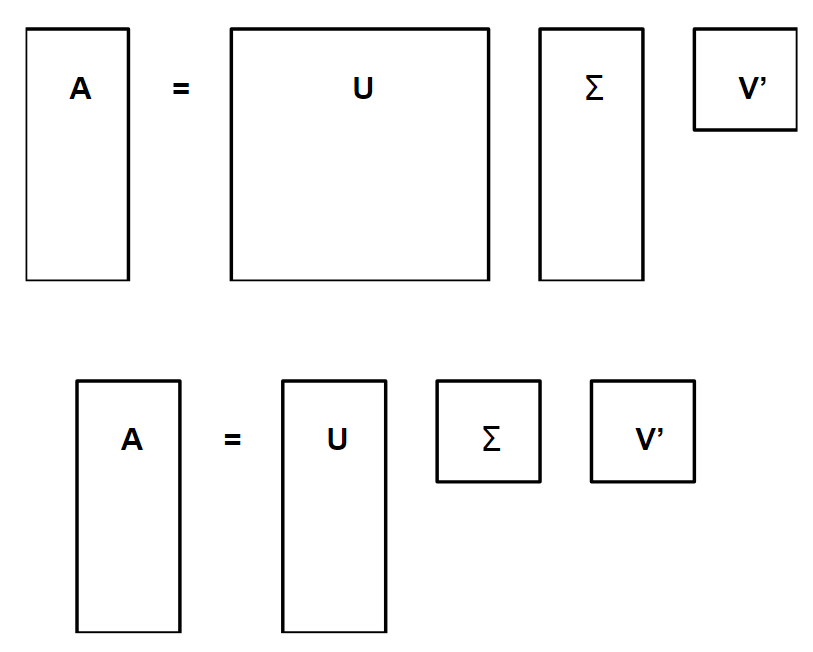
\includegraphics[height=5.5cm]{full_and_trunc_svd.PNG}
    \caption{SVD component matrices visualised, full (above) and "economy", i.e. truncated to rank $r$ (below).}
    \label{fig:svd_vis_01}
\end{figure}

%%%%%%%%%%%%%%%%%%%%%%%%%%%%%%%%%%%%%%%%%
% fancy horizontal line
{\centering
{\Large \adforn{64}\rule{0.3\textwidth}{0.4pt}\hspace{0.2cm} \adforn{32}\adforn{7}\adforn{60} \hspace{0.2cm} \rule{0.3\textwidth }{0.4pt}\adforn{36}}\par
}
%%%%%%%%%%%%%%%%%%%%%%%%%%%%%%%%%%%%%%%%%

To reiterate, we have proven the \emphasis{Signular Value Decomposition} of $\B{A}$. Remember that $\B{V}$ is the eigenvector matrix of $\B{A}^T\B{A}$, $\boldsymbol{\Sigma}$ the pseudo-diagonal matrix of singular values, and $\B{U}$ the unit column space of $\B{A}$, given by $\B{Av}_i/\sigma_i$.\\
An alternative and sometimes easier way to find $\B{U},\B{V}$ is described below.
\begin{shaded*}
\begin{definition}
Matrix $\B{U}$ in  \eqref{eq:svd} is called \emphasis{\textup{left singular matrix}} and matrix $\B{V}$ is called \emphasis{\textup{right singular matrix}}.
\end{definition}
\end{shaded*}
\begin{lemma}
Matrix $\B{U}$ in  \eqref{eq:svd} (left singular) contains the unit eigenvectors of $\B{AA}^T$ as its columns and matrix $\B{V}$ contains the unit eigenvectors of $\B{A}^T\B{A}$ as its columns.
\end{lemma}
\begin{proof} \quad \\
We know from the SVD that:
\[
\B{A}=\B{U}\boldsymbol{\Sigma}\B{V}^T
\]
, where $\B{U},\B{V}$ are orthonormal and $\boldsymbol{\Sigma}^T\boldsymbol{\Sigma}$ (or equivalently $\boldsymbol{\Sigma}\boldsymbol{\Sigma}^T$) contains the eigenvalues of $\B{A}^T\B{A}$ (or $\B{AA}^T$) in its diagonal, padded with enough zeros such that its size is same $\B{A}$'s. Therefore
\[
\B{A}^T=\B{V}\boldsymbol{\Sigma}^T\B{U}^T
\]
\begin{equation}
\B{AA}^T=\B{U}\boldsymbol{\Sigma}\B{V}^T\B{V}\boldsymbol{\Sigma}^T\B{U}^T=
\B{U}\boldsymbol{\Sigma}\boldsymbol{\Sigma}^T\B{U}^T
\label{eq:svd_u_matrix}
\end{equation}
\begin{equation}
\B{A}^T\B{A}=\B{V}\boldsymbol{\Sigma}^T\B{U}^T\B{U}\boldsymbol{\Sigma}\B{V}^T=
\B{V}\boldsymbol{\Sigma}^T\boldsymbol{\Sigma}\B{V}^T
\label{eq:svd_v_matrix}
\end{equation}
It is clear from (1) that $\B{U}$ diagonalises $\B{AA}^T$ and from (2) that $\B{V}$ diagonalises $\B{AA}^T$, which concludes the proof.
\end{proof}

\begin{shaded*}
\begin{theorem}
\cite{lay}~Let $\B{A}$ be an $m \times n$ matrix with rank $r$. Then there exists an $m \times n$ matrix $\boldsymbol{\Sigma}$ that contains the $r$ singular values of $\B{A}$ ($\sigma_1,\ldots, \sigma_r$) in its diagonal padded with $m-r$ rows and $n-r$ columns of zeros
\begin{equation}
\boldsymbol{\Sigma}=
\begin{bmatrix}
\begin{array}{c|c}
\begin{matrix}\sigma_1 & & \\ & \ddots & \\ & & \sigma_r\end{matrix} & \B{0}_{r\times n-r} \\
\hline
\B{0}_{m-r\times r} & \B{0}_{m-r\times\ n-r}
\end{array}
\end{bmatrix}
\end{equation}
and there exist orthogonal matrices $\B{U}_{m \times m}$, $\B{V}_{n \times n}$ such that
\begin{equation}
\B{A}=\B{U}\boldsymbol{\Sigma}\B{V}^T, \quad 
\end{equation}
\label{theorem:svd}
\end{theorem}
\end{shaded*}

\mycomment{The SVD exists for any matrix $\B{A}$. There are no size or form restrictions.}

\begin{exmp}
Find the singular values of the matrix $\B{A}=\begin{bmatrix} 1 & 2\\2 & 1 \end{bmatrix}$\end{exmp}.
\begin{TheSolution}
\[
\B{A}^T\B{A}=\begin{bmatrix}5&4\\4&5 \end{bmatrix}
\]
Find its eigenvalues.
\[
\begin{gathered}
\textup{det}\Big(\begin{bmatrix}5&4\\4&5 \end{bmatrix} -\lambda \B{I}\Big)=0 \Rightarrow \\
\lambda^2-10\lambda+9=0\Rightarrow \\
\lambda=9 \hquad \textup{or} \hquad \lambda = 1
\end{gathered}
\]
The singular values of $\B{A}$ are $\sigma_1=\sqrt{9}, \hquad \sigma_2=\sqrt{1}$.
\end{TheSolution}

\begin{exmp}
Find the Singular Value Decomposition of matrix $\B{A}=\begin{bmatrix}4 & 11 & 14\\8 & 7 & -2\end{bmatrix}$. ~\cite{lay}\\
\end{exmp}\begin{TheSolution}
Find $\B{A}^T\B{A}$ and its eigen-data.
\[
\B{A}^T\B{A}=10\begin{bmatrix}8 & 10 & 4\\10 & 17 & 14\\4 & 14 & 20 \end{bmatrix}
\]
The eigenvalues in decreasing order are $\lambda_1=360,\lambda_2=90,\lambda_3=0$ therefore the singular values are $\sigma_1=\sqrt{360},\sigma_2=\sqrt{90},\sigma_3=0$. If we created a diagonal matrix with the non-zero eigenvalues it would be $2 \times 2$. We pad with zeros to make it $2 \times 3$.
\[
\boldsymbol{\Sigma}=\begin{bmatrix}\sigma_1 & 0 & 0\\0 & \sigma_2 & 0\end{bmatrix}=\begin{bmatrix}\sqrt{360} & 0 & 0\\0 & \sqrt{90} & 0\end{bmatrix}
\]
The corresponding eigenvectors are
\[
\B{V}=\begin{bmatrix}\B{v}_1 & \B{v}_2 & \B{v}_3 \end{bmatrix}=
\begin{bmatrix}1/3 & -2/3 &2/3\\2/3&-1/3&-2/3\\2/3&2/3&1/3 \end{bmatrix}
\]
$\B{AA}^T$ is small ($2 \times 2)$ so we could find its unit eigenvectors from  \eqref{eq:svd_u_matrix} to construct $\B{U}$.
\[
\B{AA}^T=\begin{bmatrix}333 & 81\\81 & 117 \end{bmatrix}, 
\quad \lambda_1=360:\hquad \B{u}_1 = \begin{bmatrix}0.948 \\ 0.316\end{bmatrix}, \quad
\quad \lambda_2=90:\hquad \B{u}_2 = \begin{bmatrix}0.316 \\ -0.948\end{bmatrix}
\]
\[
\therefore \B{U}=\begin{bmatrix} 0.948 & 0.316\\0.316 & -0.948\end{bmatrix}
\]
An alternative way to construct $\B{U}$ would be using  \eqref{eq:svd_ui_vector}. Verify that they are the same. 
\[
\begin{gathered}
\B{u}_1 = \frac{\B{Av}_1}{\sigma_1}=\ldots\\
\B{u}_1 = \frac{\B{Av}_2}{\sigma_2}=\ldots
\end{gathered}
\]

Finally, we have the SVD decomposition
\[
\B{A}=\B{U}\boldsymbol{\Sigma}\B{V}^T=\begin{bmatrix} 0.948 & 0.316\\0.316 & -0.948\end{bmatrix}\begin{bmatrix}\sqrt{360} & 0 & 0\\0 & \sqrt{90} & 0\end{bmatrix}\begin{bmatrix}1/3 & 2/3 &2/3\\-2/3&-1/3&2/3\\2/3&-2/3&1/3 \end{bmatrix}
\]
The last equation is easy to numerically verify e.g. with Matlab.
\end{TheSolution}


\begin{exmp}
Compute the SVD of the matrix $\B{A}=\begin{bmatrix}1 & 1\\1& 0\\0 & 1 \end{bmatrix}$ \cite{pres_bingham}.

\end{exmp}
\begin{TheSolution}
\[
\B{A}^T\B{A}=\begin{bmatrix}2 &  1\\1 &2 \end{bmatrix}
\]
Eigenvalues and unit eigenvectors:
\[
\lambda_1:\; \B{v}_1=\begin{bmatrix}1\sqrt{2} \\1\sqrt{2} \end{bmatrix}, \quad
\lambda_2:\; \B{v}_2=\begin{bmatrix}-1\sqrt{2} \\1\sqrt{2} \end{bmatrix}
\]
The unit eigenvectors of $\B{A}^T\B{A}$ are the columns of the right singular matrix $\B{V}$:
\[
\B{V}=\begin{bmatrix}1\sqrt{2} & -1\sqrt{2}\\1\sqrt{2}& 1\sqrt{2} \end{bmatrix}
\]
The square roots of the eigenvalues of $\B{A}^T\B{A}$ are the diagonal entries of $\boldsymbol{\Sigma}$:
\[
\boldsymbol{\Sigma}=\begin{bmatrix}\sqrt{3} & 0\\0 & 1\\ 0 & 0 \end{bmatrix}
\]
Finally, use \eqref{eq:svd_ui_vector} to compute the left singular matrix $\B{U}$.
\[
\B{u}_1=\frac{\B{A}\B{v}_1}{\sigma_1}=
\frac{1}{\sqrt{3}}
\left(
\begin{bmatrix}1 & 1\\1& 0\\0 & 1 \end{bmatrix}
\begin{bmatrix}\tfrac{1}{\sqrt{2}} \\ \tfrac{1}{\sqrt{2}} \end{bmatrix}
\right)=
\begin{bmatrix}
\sqrt{\tfrac{2}{3}} \\
\tfrac{1}{\sqrt{6}}\\
\tfrac{1}{\sqrt{6}}
\end{bmatrix}
\]
\[
\B{u}_2=\frac{\B{A}\B{v}_2}{\sigma_2}=
\frac{1}{1}
\left(
\begin{bmatrix}1 & 1\\1& 0\\0 & 1 \end{bmatrix}
\begin{bmatrix}-\tfrac{1}{\sqrt{2}} \\ \tfrac{1}{\sqrt{2}} \end{bmatrix}
\right)=
\begin{bmatrix}
0 \\
-\tfrac{1}{\sqrt{2}}\\
\tfrac{1}{\sqrt{2}}
\end{bmatrix}
\]
Therefore the $\B{U}$ matrix is
\[
\B{U}=
\begin{bmatrix}
\sqrt{\tfrac{2}{3}} & 0 \\
\tfrac{1}{\sqrt{6}} & -\tfrac{1}{\sqrt{2}}\\
\tfrac{1}{\sqrt{6}} & \tfrac{1}{\sqrt{2}}
\end{bmatrix}
\]
We have run into the problem described in the comment in the theory - $\B{U}$ is not square therefore the SVD multiplication is impossible. We want to make it a $3 \times 3$ orthonormal matrix. The way to do this is by picking a random vector (a good idea is one with a lot of zeros) in the plane spanned by the columns of $\B{U}$, i.e. in $\setR^3$. We pick
\[
\B{y}=\begin{bmatrix}1 \\ 0 \\ 0\end{bmatrix}
\]
Use the Gram-Schmid formula in  \eqref{eq:svd_gs} to construct an orthonormal basis $\B{u}_1,\B{u}_2,\B{u}_3$ in $\setR^3$ starting from $\B{u}_1,\B{u}_2$.
\[
\begin{gathered}
\B{u}_3=\B{y} - \frac{\B{y}\cdot\B{u}_1}{\B{u}_1\cdot\B{u}_1}\B{u}_1 - \frac{\B{y}\cdot\B{u}_2}{\B{u}_2\cdot\B{u}_2}\B{u}_2=
\begin{bmatrix} \tfrac{1}{3} \\ -\frac{1}{3} \\-\tfrac{1}{3} \end{bmatrix}, \\
\frac{\B{u}_3}{\norm{\B{u}_3}}=
\begin{bmatrix}\tfrac{1}{\sqrt{3}} \\ -\frac{1}{\sqrt{3}} \\-\tfrac{1}{\sqrt{3}} \end{bmatrix}
\end{gathered}
\]
Therefore we have computed the left singular matrix and everything required for the SVD.
\[
\B{U}=\begin{bmatrix}
\sqrt{\tfrac{2}{3}} & 0 & \tfrac{1}{\sqrt{3}} \\
\tfrac{1}{\sqrt{6}} & -\tfrac{1}{\sqrt{2}} &  -\frac{1}{\sqrt{3}}\\
\tfrac{1}{\sqrt{6}} & \tfrac{1}{\sqrt{2}} & -\tfrac{1}{\sqrt{3}}
\end{bmatrix}
\]
To sum up:
\[
\begin{gathered}
\B{A}=\B{U}\boldsymbol{\Sigma}\B{V}^T \Leftrightarrow\\
\begin{bmatrix}1 & 1\\1& 0\\0 & 1 \end{bmatrix}=
\begin{bmatrix}
\sqrt{\tfrac{2}{3}} & 0 & \tfrac{1}{\sqrt{3}} \\
\tfrac{1}{\sqrt{6}} & -\tfrac{1}{\sqrt{2}} &  -\frac{1}{\sqrt{3}}\\
\tfrac{1}{\sqrt{6}} & \tfrac{1}{\sqrt{2}} & -\tfrac{1}{\sqrt{3}}
\end{bmatrix}
\begin{bmatrix}\sqrt{3} & 0\\0 & 1\\ 0 & 0 \end{bmatrix}
\begin{bmatrix}1\sqrt{2} & -1\sqrt{2}\\1\sqrt{2}& 1\sqrt{2} \end{bmatrix}^T
\end{gathered}
\]
\qedblack\\\end{TheSolution}
\mycomment{ % my comment
We saw in the last example that the SVD had the form
\[
\B{A}=
\begin{bmatrix}\B{u}_1 & \B{u}_2 & \B{u}_3\end{bmatrix}
\begin{bmatrix}\sigma_1 & 0\\ 0 & \sigma_2\\0 & 0 \end{bmatrix}
\begin{bmatrix}\B{v}_1^T \\ \B{v}_2^T \end{bmatrix}
\]
And expanding the matrix product for $\B{A}$ into a sum:
\[
\begin{split}
\B{A}&=
\sqrt{3}
\begin{bmatrix}\sqrt{\tfrac{2}{3}}\\\tfrac{1}{\sqrt{6}}\\\tfrac{1}{\sqrt{6}} \end{bmatrix}
\begin{bmatrix}\tfrac{1}{\sqrt{2}} & \tfrac{1}{\sqrt{2}} \end{bmatrix} + 
1
\begin{bmatrix}0 \\ -\tfrac{1}{\sqrt{2}}\\ \tfrac{1}{\sqrt{2}} \end{bmatrix}
\begin{bmatrix}-\tfrac{1}{\sqrt{2}} & \tfrac{1}{\sqrt{2}} \end{bmatrix}\\
&=\sqrt{3}
\myunderbrace{\begin{bmatrix}\tfrac{1}{\sqrt{3}} & \tfrac{1}{\sqrt{3}} \\ \tfrac{1}{\sqrt{12}} & \tfrac{1}{\sqrt{12}} \\ \tfrac{1}{\sqrt{12}} & \tfrac{1}{\sqrt{12}}\end{bmatrix} }{\B{A}_1}
+
\myunderbrace{\begin{bmatrix}0 & 0\\ \tfrac{1}{2} & -\tfrac{1}{2}\\ -\tfrac{1}{2} & \tfrac{1}{2} \end{bmatrix}}{\B{A}_2}
\end{split}
\]
So $\B{A}$ is written as a linear combination of two rank-one matrices. Their rank is not a coincidence and why it's $1$ is explained below. The first term gives a better approximation to $\B{A}$ than the second as its weight ($\sigma_1$) is higher. Remember that singular values are in non-decreasing order. Let $\tilde{\B{A}}_1,\tilde{\B{A}}_2$ be the approximations of $\B{A}$ by the first and second term respectively, then we can see $\tilde{\B{A}}_1$ is closer to the original matrix.
\[
\tilde{\B{A}}_1=\begin{bmatrix}1 & 1\\ \tfrac{1}{2} & \tfrac{1}{2}\\ \tfrac{1}{2} \tfrac{1}{2}\end{bmatrix},\quad
\tilde{\B{A}}_2=\begin{bmatrix}0 & 0\\ \tfrac{1}{2} & -\tfrac{1}{2}\\ -\tfrac{1}{2} & \tfrac{1}{2} \end{bmatrix}
\]
} % end mycomment
Approximating a matrix by using the product of the first $k$ values, left and right singular vectors and ignoring the remaining products is called \emphasis{low rank approximation}.
\begin{shaded*}
\begin{definition}
If $\B{u} \in \setR ^m$ and $\B{v} \in \setR^n$ then the product $\B{u}\B{v}^T$ is called \textup{\emphasis{outer product}}. It yields an $m \times n$ matrix whose rank is $1$.
\end{definition}
\end{shaded*}
\begin{proof} \quad \\
Let the product be $\B{A}$.
\[
\B{A}=\B{u}\B{v}^T=\begin{bmatrix}u_1\B{v}^T \\ \vdots \\ u_m\B{v}^T \end{bmatrix}
\]
So the rows are all linearly dependent and by Gaussian elimination we can only leave $u_1\B{v}^T$, i.e. $rank(\B{A})=1$ \cite{lec_notes_roughgarden}.
\end{proof}
\begin{proof} \quad \\
Take a vector $\B{x} \in \setRn$. Then the outer product matrix maps it to another vector in $\setRn$.
\[
\B{A}\B{x}=(\B{u}\B{v}^T)\B{x}=\B{u}(\B{v}^T\B{x})=k\B{u}
\]
$k=\B{v}^T\B{x}$ is a scalar, particularly it is a dot product $((1\times n) \times (n \times 1) \rightarrow 1)$. Hence $rank(\B{A})=dim\left(\mathcal{R}(\B{A})\right)=1$~\cite{stackexch_rank_one}.
\end{proof}
Outer products are useful as they appear in the expanded SVD before the low rank approximation we will discuss the geometry of SVD.


\subsubsection{Geometric interpretation of SVD} 

We reiterate SVD's equation.
\[
\B{A}=\B{U}\boldsymbol{\Sigma}\B{V}^T
\]
We will consider the product
\[
\B{A}\B{x}=\B{U}\boldsymbol{\Sigma}\B{V}^T\B{x}, \hquad \norm{\B{x}}=1
\]
We know that orthogonal matrices represent rotations (Appendix \ref{app:orthog_and_rotations}. If $\B{A}$ is $m \times n$, then $\B{U}$ is $m \times m$, $\boldsymbol{Sigma}$ is $m \times n$ and $\B{U}$ is $n \times n$. As we will see, SVD specifies that every linear transformation is fundamentally a rotation or reflection, followed by a scaling, followed by another rotation or reflection~\cite{lec_notes_geijin}.
\begin{enumerate}
\item A rotation of vectors in the $n$-dimensional domain represented by matrix $\B{V}$
\item A linear dilation or contraction (essentially scalar multiplication) along each of the $m$ coordinate directions represented by $\boldsymbol{\Sigma}$.
\item A rotation of vectors in the $m$-dimensional range represented by $\B{U}$.
\end{enumerate}
Below is a visualisation of those actions for a $2 \times 2$ matrix operator $\B{A}$ on unit column vector $\begin{bmatrix}x_1 & x_2 \end{bmatrix}^T$. In the illustration both rotations are in $\setR^2$ but they could be in different dimensions.
\begin{figure}[H]
	\centering %centralizar a figura
	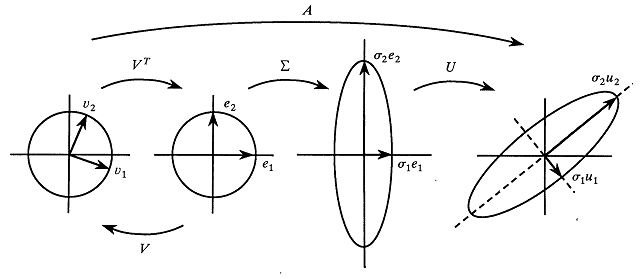
\includegraphics[height=4.25cm]{SVD_visual_01.png}
    \caption{Linear transform from $\setR^2$ to $\setR^2$~\cite{strang09}.}
    \label{fig:circle_to_ellipse_example}
\end{figure}
We also know from Section 4, \eqref{eq:max_min}, that the maximum value of $\norm{\B{Ax}}$ is $\sqrt{\lambda_1}=\sigma_1$ and the minimum $\sqrt{\lambda_1}=\sigma_1,\hquad \lambda_1 \geq \lambda_2 \geq 0$. Therefore SVD transform the unit circle in this case (or "unit sphere" in general).

\begin{exmp}
If $\B{A}=\begin{bmatrix}4 & 11 & 14\\8 & 7& -2 \end{bmatrix}$\ then the transform $\B{x}\rightarrow \B{Ax}$ maps the unit shpere $\B{x}: \norm{\B{x}}=1$ in $\setR^3$ onto an ellipse in $\setR^2$, as shown in Fig. \ref{fig:circle_to_ellipse_example}. Find the unit vectors for which $\norm{\B{Ax}}$ and compute the minimum and maximum lengths.
\begin{figure}[H]
	\centering %centralizar a figura
	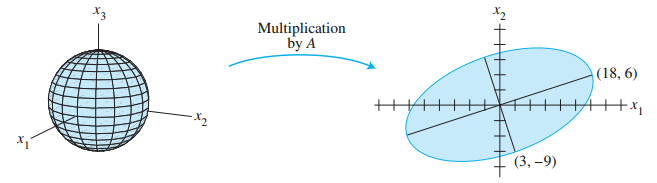
\includegraphics[height=3.75cm]{sphere_to_ell.PNG}
    \caption{SVD consists of 3 action; rotation in one domain, followed by scaling, followed by rotation in another domain~\cite{lay}.}
    \label{fig:svd_vis_01}
\end{figure}
\end{exmp}
\begin{TheSolution}
From Section 4, $\norm{\B{Ax}}$ is maximised (minimised) for the eigenvector corresponding to the maximum (minimum) non-zero eigenvalue $\lambda_1$ ($\lambda_i,\hquad i>1$) of $\B{A}^T\B{A}$.
\[
\B{A}^T\B{A}=10\begin{bmatrix}8 & 10 & 4\\10 & 17 & 14\\4 & 14 & 20 \end{bmatrix}
\]
Eigen-data:
\[
{{\lambda }_{1}}=360:{{\B{v}}_{1}}=\begin{bmatrix}
   1/3  \\
   2/3  \\
   2/3  \\
\end{bmatrix} ,\ {{\lambda }_{2}}=90:{{\B{v}}_{2}}=\left[ \begin{matrix}
   -2/3 \\
   -1/3  \\
   2/3 \\
\end{matrix} \right],\ \ {{\lambda }_{3}}=0:{{\B{v}}_{3}}=\left[ \begin{matrix}
   -2/3  \\
   2/3  \\
   -1/3  \\
\end{matrix} \right]
\]

We then find that $\underset{\left\| \B{x} \right\|=1}{\mathop{\max }}\,\left( \B{Ax}\right)=6\sqrt{10},\underset{\left\| \B{x} \right\|=1}{\mathop{\min }}\,\left( \B{Ax} \right)=\sqrt{90}$.\\
We will find how the transform $\B{x} \mapsto \B{Ax},\norm{\B{x}}=1$ maps vector $\B{x}$ to. From SVD we know:
\[
\B{A}\B{V}=\boldsymbol{\Sigma}\B{U}
\]
We know that
\[
\begin{gathered}
\B{A}\B{v}_1=\begin{bmatrix}18 \\ 6 \end{bmatrix} , \hquad
\B{A}\B{v}_2=\begin{bmatrix}3 \\ -9 \end{bmatrix}, \hquad
\B{A}\B{v}_3=\begin{bmatrix}0 \\ 0\end{bmatrix} 
\end{gathered}
\]
So we write the coordinate vector $\B{x}$ in terms of the basis $\B{v}_1,\B{v}_2,\B{v}_3$:
\[
\B{x}=x_1\B{v}_1 + x_2\B{v}_2 + x_3\B{v}_3
\]
A general point given by the vector $x_1\B{v}_1+x_2\B{v}_2+x_3\B{v}_3$is mapped to
\[
\B{A}\B{V}\B{x}=\begin{bmatrix}18x_1+3x_2\\6x_1-9x_2 \end{bmatrix}
\]
Because $\B{x}$ is on the unit sphere, we can parametrise it as $(x_1,x_2,x_3)=(r\cos \theta, r\sin \theta,z)$, so the polar coordinates w.r.t. $\B{v}_1,\B{v}_2,\B{v}_3$ are
\[
\begin{split}
\B{A}\B{V}\B{x}&=\begin{bmatrix}r18\cos\theta+r3\sin\theta\\r6\cos\theta-r9\sin\theta \end{bmatrix} \\
&= \begin{bmatrix}r6\sqrt{10}cos(\alpha-\theta)\\ r3\sqrt{10}sin(\alpha-\theta) \end{bmatrix}
\end{split}
\]
In vector notation, we have the mapping $\left(\sin(\theta),\cos(\theta),z\right) \mapsto \left(r6\sqrt{10}cos(\alpha-\theta), r3\sqrt{10}sin(\alpha-\theta)\right)$, where $r=1$ because $\B{x}$ is on the unit sphere. For example, point $(0,0,1)$ maps to $(0,0)$ \cite{stackexch_svd_geo}.
\qedblack
\end{TheSolution}

\begin{corollary}\quad \newline
\begin{itemize}
\item As any matrix $\B{A}$ has an SVD decomposition, it will always transform the "unit sphere" (hypershphere) into an ellipsoid.
\item If $\B{A}$ does not have full rank, then some of the semi-axes of the transformed ellipsoid will have length 0.
\end{itemize}
\end{corollary}
To formalise what was observed in the last example, if we have a matrix $\B{A}=\B{U}\boldsymbol{\Sigma}\B{V}^T$, a coordinates vector on the unit sphere in $\setR^n$  and express it w.r.t. right singular vectors $\B{V}$, i.e. 
\[
\left \{ \B{x}=x_1\B{v}_1 + x_2\B{v}_2 + \ldots + x_n\B{v}_n  \hquad \left| \hquad \sum\limits_{i=1}^{n}{x_{i}^{2}} \right.  \right \}
\]
Then from SVD we know that the image of $\B{x}$ is
\[
\B{Ax}=\sum\limits_{i=1}^{r=rank\left( \mathbf{A} \right)}{{{\sigma }_{i}}{{\mathbf{u}}_{i}}\mathbf{v}_{i}^{T}{{\mathbf{v}}_{i}}{{x}_{i}}}=\sum\limits_{i=1}^{r=rank\left( \mathbf{A} \right)}{{{\sigma }_{i}}{{\mathbf{u}}_{i}}{{x}_{i}}}
\]
Letting $y_i=\sigma_i\B{x}_i$, we see that the image of the unit sphere consists of the vectors $\B{y}_1\B{u}_1 + \B{y}_2\B{u}_2 + \ldots + \B{y}_r\B{u}_r$, where~\cite{lec_notes_kalman}
\[
\begin{split}
\frac{y_{1}^{2}}{\sigma _{1}^{2}}+\frac{y_{2}^{2}}{\sigma _{2}^{2}}+\ldots +\frac{y_{r}^{2}}{\sigma _{r}^{2}} &= \sum\limits_{i=1}^{r}{x_{i}^{2}} \\
& \leq 1
\end{split}
\]
If $\B{A}$ has full column rank, so $r=n$ the inequality is actually a strict equality.  Otherwise, some of the $x_i$ are missing on the right, and the sum can be anything from 0 to 1. This leads to the next corollary.

\begin{corollary}
$\B{A}$ maps the  unit  sphere  of $\setRn$ to  a k-dimensional  ellipsoid  with  semi-axes  in  the  directions $\B{u}_i$ and  with  the magnitudes $\sigma_i$. If $r=n$ the image is just the surface of the ellipsoid, otherwise it is the solid ellipsoid. In summary, we can visualize the effect of $\B{A}$ follows:  \\
It first collapse $n-r$ dimensions of the domain,then  distorts  the  remaining  dimensions,  stretching  and  squeezing  the  unit r-sphere  into  an  ellipsoid,and finally embeds the ellipsoid in $\setR ^ m$.
\end{corollary}



\subsection{Application 1: SVD and fundamental subspaces}
Motivated by the $\boldsymbol{\Sigma}$ matrix partitioning in the SVD Theorem \ref{theorem:svd}, we can partition $\B{U}$ and $\B{V}$ in a similar way. Let $\B{A}$ be $m \times n$, then, denoting $\boldsymbol{\Sigma}_r = \textup{diag}(\sigma_1,\ldots , \sigma_r)$ \cite{lec_notes_hyde}.
% TODO: yup that's ugly

\begin{align}
\B{A} &= \begin{bmatrix}\myunderbrace{\hquad \B{U}_1  \hquad}{m \times r} & \myunderbrace{\hquad \ \B{U}_2 \hquad \ }{m \times m-r} \end{bmatrix}
\begin{bmatrix}
\begin{array}{c|c}
\boldsymbol{\Sigma}_r & \B{0}_{r\times n-r} \\
\hline
\B{0}_{m-r\times r} & \B{0}_{m-r\times\ n-r}
\end{array}
\end{bmatrix}
\begin{bmatrix}\myunderbrace{\hquad \B{V}_1  \hquad}{m \times r} & \myunderbrace{\hquad \ \ \B{V}_2 \hquad \ \ }{n \times n-r} \end{bmatrix}^T \nonumber \\
& = \begin{bmatrix}\myunderbrace{\hquad \B{U}_1\boldsymbol{\Sigma}_r  \hquad}{m \times r} & \myunderbrace{\hquad \ \ \B{0} \hquad \ \ }{m \times n-r}  \end{bmatrix} 
\begin{bmatrix}\myunderbrace{\hquad \B{V}_1^T \hquad}{r \times n} \\
\myunderbrace{\hquad \B{V}_2^T \hquad}{n-r \times n } 
\end{bmatrix} \nonumber \\
&= \underset{m\times r}{\mathop{{{\mathbf{U}}_{1}}}}\, \ \underset{r\times r}{\mathop{{{\mathbf{\Sigma }}_{r}}}}\, \ \underset{r\times n}{\mathop{{{\mathbf{V}}_{1}^T}}}\ 
\label{eq:svd_compact}
\end{align}
\eqref{eq:svd_compact} is a more compact form of SVD for full rank.
\begin{corollary}
Suppose $\B{A}$ is any $n \times n$ matrix, and $\B{A}=\B{U}_1\boldsymbol{\Sigma}_r\B{V}_1$ is the full rank SVD.  It follows that an orthonormal set of basis vectors for the range (or column space) $\mathcal{R}(\B{A})$ of $\B{A}$ are the columns of $\B{U}_1$\cite{lec_notes_hyde}.
\end{corollary}
\begin{proof}
When $\B{b} \in \mathcal{R}(\B{A})$ (in the column space) then for some vector $\B{x}$:
\[
\B{b} = \B{Ax} = \B{U}_1\boldsymbol{\Sigma}_r\B{V}_1^T \B{x} = \B{U}_1 \B{x}^{\star}
\]
, where $\B{x}^{\star}=\boldsymbol{\Sigma}_r\B{V}_1^T \B{x} $ is an $r \times 1$ vector. Therefore also $\B{b} \in \mathcal{R}(\B{U}_1) $, which means  
\[
\mathcal{R}(\mathbf{A})\supseteq \mathcal{R}({{\mathbf{U}}_{1}})
\tag{1}
\label{eq:svd_col_space_1}
\]
Since $\boldsymbol{\Sigma}_r$ is invertible and symmetric and $\B{V}_1$ is orthonormal:
\begin{align*}
\B{U}_1\boldsymbol{\Sigma}_r\B{V}_1^T = \B{A} \Longrightarrow \B{U}_1 = \B{A}\B{V}_1\boldsymbol{\Sigma}_r^{-1}
\end{align*}
If $\B{b} \in \mathcal{R}(\B{U}_1)$, then for some vector $\B{y}$:
\[
\B{b} = \B{U}_1\B{y} = \B{A}\B{V}_1\boldsymbol{\Sigma}_r^{-1} \B{y} = \B{A} \B{y}^{\star}
\]
Therefore also $\B{y} \in \mathcal{R}(\B{A})$, which means 
\[
\mathcal{R}(\mathbf{A})\subseteq \mathcal{R}({{\mathbf{U}}_{1}})
\tag{2}
\label{eq:svd_col_space_2}
\]
From \eqref{eq:svd_col_space_1}, \eqref{eq:svd_col_space_2} we have $\mathcal{R}({{\mathbf{U}}_{1}})=\mathcal{R}(\B{A})$. Since $\B{U}_1$ is an orthonormal set, column vectors in $\B{U}_1$ are an orthonormal basis for $\mathcal{R}(\B{A})$.
\end{proof}
In a similar fashion, we can prove the following.
\begin{corollary}
Suppose $\B{A}$ is any $n \times n$ matrix, and $\B{A}=\B{U}_1\boldsymbol{\Sigma}_r\B{V}_1$ is the full rank SVD.  It follows that an orthonormal set of basis vectors for the row space $\mathcal{R}(\B{A}^T)$ of $\B{A}$ are the columns of $\B{V}_1$\cite{lec_notes_hyde}.
\end{corollary}
For the null space of $\B{B}$ we have.
\begin{corollary}
Suppose $\B{A}$ is any $m \times n$    rank $r$ matrix, and $\B{A}=\B{U}\boldsymbol{\Sigma}\B{V}^T$ is the SVD.  Partition $\B{U}$ into $\begin{bmatrix}\B{U}_1 \B{U}_2 \end{bmatrix}$, where $\B{U}_1 $ is the first $r$ columns of $\B{U}$, $\B{U}_2$ is the last $m-r$ columns of $\B{U}$.  Similarly, partition $\B{V}$ as $\begin{bmatrix}\B{V}_1 \B{V}_2 \end{bmatrix}$.  It follows that an orthonormal set of basis vectors for $N(\B{A})$  are the columns of $\B{V}_2$. 
\end{corollary}
\begin{proof}
Solving \eqref{eq:svd_compact} for $\boldsymbol{\Sigma}$:
\[
\mathbf{\Sigma }=\left[ \begin{matrix}
   \underset{r\times r}{\mathop{{{\mathbf{\Sigma }}_{r}}}}\, & \underset{r\times n-r}{\mathop{\mathbf{0}}}\,  \\
   \underset{m-r\times r}{\mathop{\mathbf{0}}}\, & \underset{m-r\times n-r}{\mathop{\mathbf{0}}}\,  \\
\end{matrix} \right]=\left[ \begin{matrix}
   \underset{r\times m}{\mathop{\mathbf{U}_{1}^{T}}}\,  \\
   \underset{m-r\times m}{\mathop{\mathbf{U}_{2}^{T}}}\,  \\
\end{matrix} \right]\mathbf{A}\left[ \begin{matrix}
   \underset{n\times r}{\mathop{{{\mathbf{V}}_{1}}}}\, & \underset{n\times n-r}{\mathop{{{\mathbf{V}}_{2}}}}\,  \\
\end{matrix} \right]=\left[ \begin{matrix}
   \mathbf{U}_{1}^{T}\mathbf{A}{{V}_{1}} & \mathbf{U}_{1}^{T}\mathbf{A}{{V}_{2}}  \\
   \mathbf{U}_{2}^{T}\mathbf{A}{{V}_{1}} & \mathbf{U}_{2}^{T}\mathbf{A}{{V}_{2}}  \\
\end{matrix} \right]
\tag{3}
\label{eq:svd_nullspace_1}
\]
The partitioned sub-matrices between $\boldsymbol{\Sigma}_r$ must match each other (do the multiplications and find the dimensions of $\mathbf{U}_{i}^{T}\mathbf{A}{{V}_{i}}$) therefore we must have:
\[
\begin{bmatrix}
\mathbf{U}_{1}^{T}\mathbf{A}{{V}_{2}}\\ \mathbf{U}_{2}^{T}\mathbf{A}{{V}_{2}}
\end{bmatrix} = 
\B{0} \Longrightarrow 
\begin{bmatrix} \B{U}_1^T \\ \B{U}_2^T \end{bmatrix}\B{A}\B{V}_2 = \B{0} \Longrightarrow
\B{U}^T \B{A} \B{V}_2 = \B{0} \Longrightarrow \B{AV}_2 = \B{0}
\]
Therefore every column vector $\B{v}_{2,i}$ of $\B{V}_2$ is in the null space of $\B{A}$ and also the columns of $\B{V}_2$ form an orthonormal basis. Finally, we know $\textup{dim}(N(\B{A})) = n - r = \textup{dim}(\B{V}_2)$, so it follows that the columns of $\B{V}_2$ form a basis for $N(\B{A})$.
\end{proof}
A similar result can be derived for the left null space, or the null space of $\B{A}^T$, i.e. for all vectors such that $\B{A}^T\B{v}=0$
\begin{corollary}
Suppose $\B{A}$ is any $m \times n$    rank $r$ matrix, and $\B{A}=\B{U}\boldsymbol{\Sigma}\B{V}^T$ is the SVD.  Partition $\B{U}$ into $\begin{bmatrix}\B{U}_1&  \B{U}_2 \end{bmatrix}$, where $\B{U}_1 $ is the first $r$ columns of $\B{U}$, $\B{U}_2$ is the last $m-r$ columns of $\B{U}$.  Similarly, partition $\B{V}$ as $\begin{bmatrix}\B{V}_1 & \B{V}_2 \end{bmatrix}$, where $\B{V}_1 $ is the first $r$ columns of $\B{U}$, $\B{V}_2$ is the last $n-r$ columns of $\B{U}$.  It follows that an orthonormal set of basis vectors for the left null space of $\B{A}$ $\fancyN(\B{A}^T)$  are the columns of $\B{U}_2$ \cite{lec_notes_hyde}.
\end{corollary}
\begin{proof}
Work similarly to the null space proof. Setting $\begin{bmatrix} \mathbf{U}_{2}^{T}\mathbf{A}{{V}_{1}} & \mathbf{U}_{2}^{T}\mathbf{A}{{V}_{2}} \end{bmatrix} = \begin{bmatrix}\B{0} & \B{0} \end{bmatrix}$ we conclude that $\B{A}^T\B{U}_2 = 0$.\\
Therefore every column vector $\B{u}_{2,i}$ of $\B{U}_2$ is in the left null space of $\B{A}$ and also the columns of $\B{U}_2$ form an orthonormal basis. We know $\textup{dim}(N(\B{A}^T)) = m - r = \textup{dim}(\B{U}_2)$, so it follows that the columns of $\B{U}_2$ form a basis for $\fancyN(\B{A}^T)$.
\end{proof}
To summarise, the last four corollaries provide a standard way of finding orthonormal bases for the four fundamental subspaces.
\begin{shaded*}
\begin{theorem}
Defining the SVD of $\B{A}$ as in \eqref{eq:svd_compact} as
\[
\B{A}=\B{U}\boldsymbol{\Sigma}\B{V}^T= 
\begin{bmatrix}\B{U}_1 & \B{U}_2 \end{bmatrix}\boldsymbol{\Sigma}\begin{bmatrix}\B{V}_1 & \B{V}_2 \end{bmatrix}^T
\]
It follows that
\begin{itemize}
\item $\B{U}_1$ forms a basis for the column space $\mathcal{R}(\B{A})$
\item $\B{U}_2$ forms a basis for the left null space $N(\B{A}^T)$
\item $\B{V}_1$ forms a basis for the row space $\mathcal{R}(\B{A}^T)$
\item $\B{V}_2$ forms a basis for the null space $N(\B{A})$
\end{itemize}

\end{theorem}
\end{shaded*}




\subsection{Application 2: Low rank approximation}

We have seen that SVD can be written as a sum of rank one matrices
\[
\mathbf{A}=\sum\limits_{i=1}^{n}{{{\sigma }_{i}}{{\mathbf{u}}_{i}}\mathbf{v}_{i}^{T}}
\]
If the rank of $\B{A}$ is $r$, then $\sigma_{r+1}=\sigma_{r+2}=\ldots=\sigma_{n}=0$ therefore
\[
\mathbf{A}=\sum\limits_{i=1}^{r}{{{\sigma }_{i}}{{\mathbf{u}}_{i}}\mathbf{v}_{i}^{T}}
\]
Sometimes we want to store smaller $\B{U},\boldsymbol{\Sigma},\B{V}$ matrices e.g. in the computer memroy so we want to approximate $\B{A}$ using the first (largest) $k$ singular values
\begin{equation}
{{\mathbf{A}}_{k}}=\sum\limits_{i=1}^{k}{{{\sigma }_{i}}{{\mathbf{u}}_{i}}\mathbf{v}_{i}^{T}}
\label{eq:svd_approx}
\end{equation}
\mycomment{The low order singular values ($\sigma_1,\sigma_2,\ldots$) carry more information that the high order ones ($\sigma_r, \sigma_{r-1},\ldots$).
} % end mycomment
The figure below shows how one approximation of the sum above is obtained as a product of a $\textup{(column)} \times \textup{(singular value)} \times \textup{(row)}$
\begin{figure}[H]
	\centering %centralizar a figura
	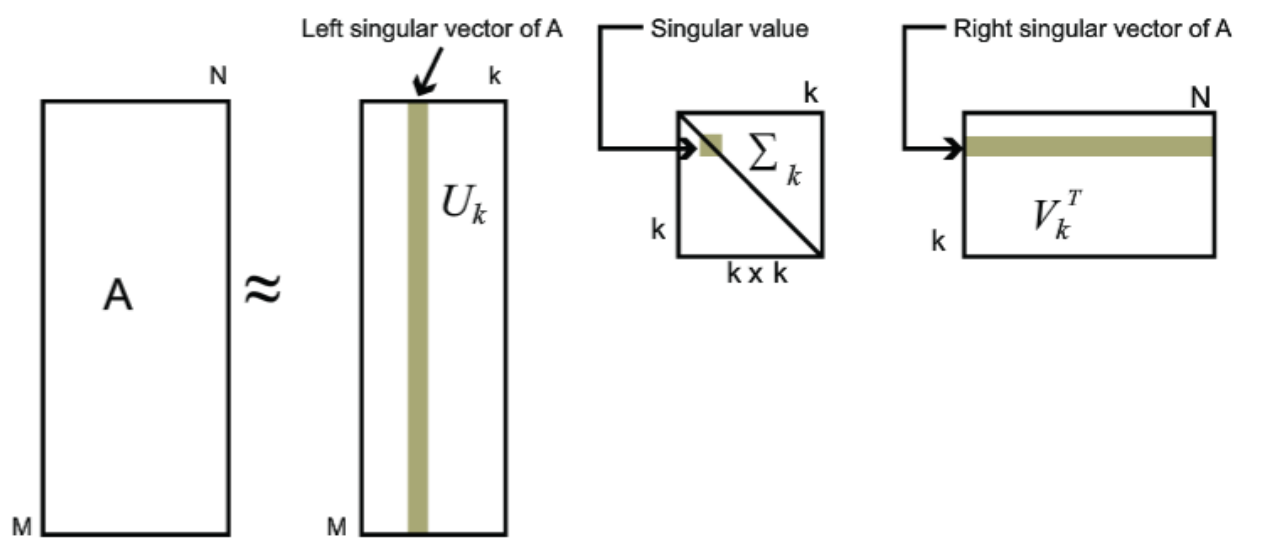
\includegraphics[height=4cm]{svd_low_rank.png}
    \caption{One term of the approximation sum in \eqref{eq:svd_approx}.}
    \label{fig:svd_approx_term}
\end{figure}



\subsubsection{SVD and norms}


To start with, an interesting result is that SVD provides the best rank $k$ approximation of a matrix $\B{A}$. The following is the 2-norm case of the \emphasis{Eckart-Young-Mirsky theorem}. We will prove it for the 2-norm first and generalise for the Frobenius norm later~\cite{lec_notes_gander}. We denote $\norm{.}$ or $\norm{.}_2$ the 2-norm.
\begin{shaded*}
\begin{theorem}
Let $\B{A}$ be an $m \times n$ matrix of rank $r$, $k<r$ and $\B{A}_k$ the rank $k$ SVD of $\B{A}$. Then for any matrix $\B{X}$ with $\textup{rank}(\B{X}) = k$
\begin{equation}
\underset{rank\left( \mathbf{X} \right)=k}{\mathop{\min }}\,\left\| \mathbf{A}-\mathbf{X} \right\|={{\sigma }_{k+1}}
\end{equation}
The equality is attained by 
\begin{equation}
\mathbf{X}={{\mathbf{A}}_{k}}=\sum\limits_{i=1}^{k}{{{\mathbf{u}}_{i}}{{\sigma }_{i}}\mathbf{v}_{i}^{T}}
\label{theorem:svd_best_approx}
\end{equation}
\end{theorem}
\end{shaded*}

\begin{proof}\quad \\
\cite{lec_notes_embree}, \cite{lec_notes_beiwang}, \cite{lec_notes_ven}~Since $\textup{rank}(\B{X})=\textup{dim}(\mathcal{R}(\B{A}))=k$, we have $\textup{dim}(N(\B{A}))=n-k$. Also, $\textup{dim}(\B{V}_{k+1})=k+1$, $\B{V}_k = \begin{bmatrix}\B{v}_1 & \ldots & \B{v}_{k+1}\end{bmatrix}$ are the first $k+1$ right singular vectors of $\B{A}$, it must be true one (call it $\B{z}$) falls in $N(\B{X})$, i.e.
\[
\exists\B{z} \in \setRn: \ \mathbf{z}\in N\left( \mathbf{X} \right)\cap span\left\{ {{\mathbf{v}}_{1}},\ldots ,{{\mathbf{v}}_{k+1}} \right\},\ \ {{\left\| \mathbf{z} \right\|}_{2}}=1 
\]
${{\left\| \mathbf{z} \right\|}_{2}}=1 $ because of course $\B{V}$ is an orthogonal matrix. We can write
\begin{align}
\B{z} = c_1 \B{v}_1 + \ldots + c_{k+1} \B{v}_{k+1} \nonumber \\ 
\therefore \norm{\B{z}} = 1 \Rightarrow \sum\limits_{i=1}^{k+1}{c_{i}^{2}}=1 \tag{1}
\label{eq:svd_norm_proof_1}
\end{align}
Using one of the properties of the 2-norm and because $\B{z} \in N(\B{X})$:
\[
\norm{\B{A} - \B{X}} \geq \norm{(\B{A} - \B{X})\B{z}} = \norm{\B{Az}}
\tag{2}
\label{eq:svd_norm_proof_2}
\]	
If we expand $\B{Az}$ using the rank-$k$ SVD of $\B{A}$ and \eqref{eq:svd_norm_proof_1} we have:
\[
\B{Az} = \left( \sum\limits_{i=1}^{k+1}{{{\sigma }_{i}}{{\mathbf{u}}_{i}}\mathbf{v}_{i}^{T}} \right)\left( \sum\limits_{j=1}^{k+1}{{{c}_{j}}{{\mathbf{v}}_{j}}} \right)=\sum\limits_{i=1}^{k+1}{{{\sigma }_{i}}{{c}_{i}}{{\mathbf{u}}_{i}}\mathbf{v}_{i}^{T}{{\mathbf{v}}_{i}}}=\sum\limits_{i=1}^{k+1}{{{\sigma }_{i}}{{c}_{i}}{{\mathbf{u}}_{i}}}
\tag{3}
\label{eq:svd_norm_proof_3}
\]
Using the orthonormality of $\B{u}_i$ and the ordering of $\sigma_i$ values:
\[
\norm{\B{Az}}^2=\sum\limits_{i=1}^{k+1}{\sigma _{i}^{2}c_{i}^{2}}\ge \sigma _{k+1}^{2}\underbrace{\sum\limits_{i=1}^{k+1}{c_{i}^{2}}}_{=\left\| {{\mathbf{z}}_{ }} \right\|=1}=\sigma _{k+1}^{2}
\tag{4}
\label{eq:svd_norm_proof_4}
\]
Therefore \eqref{eq:svd_norm_proof_2} with the aid of \eqref{eq:svd_norm_proof_3} and \eqref{eq:svd_norm_proof_4} yields the following simple expression
\[\left\| \mathbf{A}-\mathbf{X} \right\|=\underset{\left\| \mathbf{v} \right\|=1}{\mathop{\max }}\,\left\| \left( \mathbf{A}-\mathbf{X} \right)\mathbf{v} \right\|\ge \left\| \left( \mathbf{A}-\mathbf{X} \right)\mathbf{z} \right\|=\left\| \mathbf{Az} \right\|\ge \sigma _{k+1}^{2}\]
Now we want to show that the equality for minimum is obtained for $
\mathbf{X}={{\mathbf{A}}_{k}}=\sum\limits_{i=1}^{k}{{{\mathbf{u}}_{i}}{{\sigma }_{i}}\mathbf{v}_{i}^{T}} $.
\[
\B{A} - \B{A}_k=\sum\limits_{i=1}^{r}{{{\sigma }_{i}}{{\mathbf{u}}_{i}}\mathbf{v}_{i}^{T}}-\sum\limits_{i=1}^{k}{{{\sigma }_{i}}{{\mathbf{u}}_{i}}\mathbf{v}_{i}^{T}}=\sum\limits_{i=k+1}^{r}{{{\sigma }_{i}}{{\mathbf{u}}_{i}}\mathbf{v}_{i}^{T}}
\]
This is the SVD of $\B{A} - \B{A}_k$ with largest singular value $\sigma_{k+1}$ so by definition we have $\norm{\B{A} - \B{A}_k}_2=\max \left(\sum\limits_{i=k+1}^{r}{{{\sigma }_{i}}{{\mathbf{u}}_{i}}\mathbf{v}_{i}^{T}} \right)=\sigma_{k+1}$. To conclude, $\B{A}_k$ has the best norm-2 approximation.
\end{proof}

\TODO[Eckart-Young-Mirsky theorem generalisation to be written in the future.]






\subsection{Application 3: Image compression}
As mentioned before, we can only pick the first $k$ largest singular values along with the first $k$ left and right singular vectors to compress an matrix, e.g. image using less values. Particularly, if the image is $m \times n$, then we only need $m \times k + k + k \times n$ numbers to approximate the image using the SVD product. To actually save data, we want~\cite{quora_svd_jpg}
\[
k(m + n +1)<mn \Rightarrow k < \frac{mn}{m+n+1}
\]
Therefore SVD doesn't always save data, which is one of its disadvantages compares to other image compression methods such as JPG.\\
A Matlab script that performs SVD image compression is listed in App. \ref{app:svd_matlab}. Some of the results it generates are shown in the table below. Note that the rank of the cameraman image is 253 and its size is $256 \times 256$. Also, notice how Eckart-Young-Mirsky theorem is confirmed.

\begin{minipage}{\linewidth}
\captionof{table}{Approximations of the camerman image using SVD for various ranks.} \label{tab:SVD_image_results} 
\begin{center}
\begin{tabular}{| m{.125\textwidth} | m{.125\textwidth} | m{.225\textwidth}  | m{.125\textwidth} | m{.125\textwidth} | m{.125\textwidth}|}
\hline   
% image, rank, output, n required, norm 2 of difference, Singular value of rank r+1
    \textbf{Image} & \textbf{Rank} & \textbf{Output} & \textbf{Numbers required} & \textbf{Norm 2 of difference} & \textbf{Singular value r+1} \\
\hline 
\hline
Original & 253 & 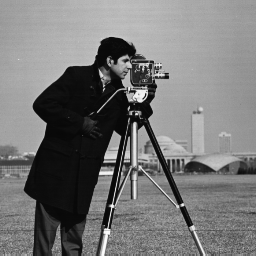
\includegraphics[scale=.27] {cameraman.png} & 65536 & &\\
\hline
Approximated & 1 & 
\includegraphics[scale=.27] {rank1.png} & 513 & 28.383 & 28.383\\
\hline
Approximated & 2 & 
\includegraphics[scale=.27] {rank2.png} & 1026 & 21.506 & 21.506\\
\hline
Approximated & 32 & 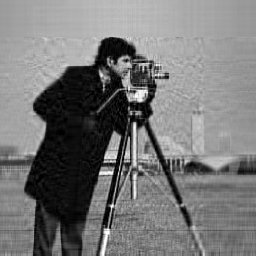
\includegraphics[scale=.27] {rank32.png} & 16416 & 2.379 & 2.379\\
\hline
Approximated & 64 & 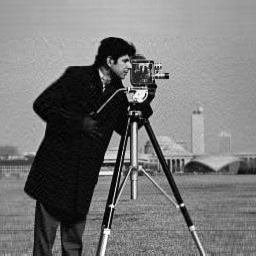
\includegraphics[scale=.27] {rank64.png} & 32832 & 1.157 & 1.157\\
\hline
\end{tabular}
\end{center}
\end{minipage}



\subsubsection{Application 3.1: Image deblurring}

\TODO[maybe in future] \\
\url{http://www.mathcs.emory.edu/~nagy/courses/fall06/ID_lecture1.pdf}



\subsection{Application 4: Pseudoinverse and least squares}

In App. \ref{app:least_squares}, we studied the system $\B{A}_{m \times n}\B{x} = \B{b}, \hquad m>n$. $\B{x} \in \setRn, \hquad \B{b} \in \setR ^ m$. Therefore in this case we have to "fit" $\B{b} \in \setR^m$ in the smaller space $\setR^n$, spanned by the columns of $\B{A}$. We "fit" $\B{b}$ by finding its smallest distance point in the column space of $\B{A}$, which is its projection on it. So instead of solving $\B{Ax}=\B{b}$ we solve $\B{A}\bar{\B{x}}=\B{p}$, there $\B{p}$ is the projection of $\B{b}$ in the column space of $\B{A}$. \\
To reiterate, we found that:
\begin{enumerate}
\item $\bar{\B{x}}$ is a least squares solution of $\B{A}\bar{\B{x}}=\B{b}$ iff $\bar{\B{x}}$ is a solution of the \textup{\emphasis{normal equations}}
\begin{equation}
\left(\B{A}^T\B{A} \right)\bar{\B{x}} = \B{A}^T\B{b}
\end{equation}
\item \B{A} has linearly independent columns if and only if $\B{A}^T\B{A}$ is invertible. In this case, the least squares solution of $\B{Ax}=\B{b}$ is unique and is given by
\begin{equation}
\bar{\B{x}} =\left(\B{A}^T\B{A} \right)^{-1} \B{A}^T\B{b}
\label{eq:svd_pseudo_1}
\end{equation}
\end{enumerate}
\mycomment{If the stability of 	the system is in doubt therefore we cannot invert $\B{A}^T\B{A}$, then we can solve the system by QR factorisation or SVD. We will study the latter. QR factorisation is essentially a compact matrix form of the Gram Schmidt decomposition, where $\B{Q}$ is orthogonal and $\B{R}$ is upper triangular. The QR solution is proven in App. \ref{app:pseudo_with_qr}} % end comment
Matrix $(\B{A}^T\B{A})^{-1}\B{A}^T$ is called \emphasis{pseudoinverse} of $\B{A}$ and we will show that it can be readily computed by SVD. The classical inverse exists only if $\B{A}$ is $n \times n$ and $\rank(\B{A})=n$. The pseudoinverse $\B{A}^{+}$ exists for all $\B{A}_{m \times n}$ matrices. It can be thought as a generalisation of the inverse. When $\B{Ax}=\B{b}$ has no solutions, which is the case we study, is provides the matrix such that $\B{A}^{+}\B{x}$ is closest to $\B{b}$. If many solutions exists, it picks the solution that minimises $\B{x}_2$.\\
Pseudoinverse does not necessarily have the strong $\B{A}^{+}\B{A}=\B{I}$ property, but satisfies all of the following properties~\cite{stackexch_pseudo_prop}.
\begin{corollary} \quad \\
\begin{enumerate}
\item $\B{A}\B{A}^+\B{A}=\B{A}$ ($\B{A}\B{A}^+$ does not have to be the identity matrix but maps all column vectors of $\B{A}$ to themselves)
\item $\B{A}^+\B{A}\B{A}^+ = \B{A}^+$
\item $(\B{A}\B{A}^+)^T=\B{A}\B{A}^+$
\item $(\B{A}^+\B{A})^T=\B{A}^+\B{A}$
\item $\rank(\B{A}^+) = \rank(\B{A})$
\end{enumerate}
Also, note that $\B{A}\B{A}^+$ and $\B{A}^+\B{A}$ are as close to $\B{I}_m$ and $\B{I}_n$ respectively as possible. 

\end{corollary}
It can easily be proven\cite{stackexch_pseudo} that the solution $\bar{\B{x}}$ in \eqref{eq:svd_pseudo_1} in terms of singular vectors and values is given by:
\begin{equation}
\bar{\B{x}} = \B{V}\B{D}^{+}\B{U}^T\B{b}, \quad \B{D}^{+} = (\B{D}^2)^{-1}\B{D}
\label{eq:svd_pseudo_2}
\end{equation}
In \eqref {eq:svd_pseudo_2}, matrix $\B{A}$ doesn't have to be invertible so that's a general way to compute its pseudo inverse. $\B{D}^+$ is of course the pseudo inverse of $\B{D}$. Consider the following cases when finding $\bar{\B{x}}$ \cite{lec_notes_georgy}.
\begin{itemize}
\item $\rank(\B{A}) = n$, i.e. $\sigma_1 \geq \ldots \geq \sigma_n > 0$. Then $\B{D}$'s pseudoinverse coincides with its inverse so it's trivial to find:
\[
\B{D}^+ = \B{D}^{-1} = \begin{bmatrix}\tfrac{1}{\sigma_1}& & \\ & \ddots & \\ & & \tfrac{1}{\sigma_n} \end{bmatrix}
\]
Then the matrix $\B{V}\B{D}^{+}\B{U}^T$ from \eqref{eq:svd_pseudo_2} is indeed the pseudoinverse of $\B{A}$ as
\[
\B{A}^T\B{A} = \B{V}\B{D}^{+}\B{U}^T\B{U}\B{D}\B{V}^T = \B{I}_n
\]
\item $\rank(\B{A}) = r < n$, therefore $\B{A}^{-1}$ does not exist. However, the pseudoinverse does exist and for each column we have:
\[
\B{A}^+\B{u}_i = \left \{ \begin{array}{ll}\tfrac{1}{\sigma_i}\B{v}_i, &  i \leq r=\rank(\B{A}) \\ 
0, & \textup{otherwise} \end{array} \right.
\]
In matrix form, this is written as
\begin{equation}
\B{A}^+ =  \B{V}\B{D}^{+}\B{U}^T, \quad \B{D}^+ = \begin{bmatrix} \sigma_1 & & \\ & \ddots & \\ & & \sigma_r\end{bmatrix} 
\end{equation}
\end{itemize}
Again, $\B{D}^+\B{D}$ is as close to the identity as possible.





\subsection{Application 5: Principal Component Analysis (PCA)}

PCA is a statistical procedure concerned with elucidating the covariance structure of a set of variables. In particular it allows us to identify the principal directions in which the data varies. To be more precise, \cite{lec_notes_gillies},
\begin{itemize}
    \item it projects data onto a lower-dimensional manifold that preserves as much information as possible,
    \item minimises reconstruction error,
    \item maximises the variance (signal) of the projected data,
    \item maximises the mutual information between original and projected data
\end{itemize}


\TODO \\
\url{http://www.cse.psu.edu/~rtc12/CSE586Spring2010/lectures/pcaLectureShort.pdf}\\
\url{https://www.ini.rub.de/PEOPLE/wiskott/Teaching/Material/PrincipalComponentAnalysis-LectureNotesPublic.pdf}\\
\url{https://alliance.seas.upenn.edu/~cis520/wiki/index.php?n=Lectures.PCA}\\
\url{https://courses.cs.washington.edu/courses/cse521/16sp/521-lecture-9.pdf}\\
\url{http://pillowlab.princeton.edu/teaching/statneuro2018/slides/notes04_PCA.pdf}\\
\url{https://www.cs.princeton.edu/picasso/mats/PCA-Tutorial-Intuition_jp.pdf} \\
\url{http://labs.seas.wustl.edu/bme/raman/Lectures/Lecture11_PCA.pdf}\\
\url{https://www.cs.cmu.edu/~elaw/papers/pca.pdf}\\
\url{http://www.cis.upenn.edu/~cis515/cis515-12-sl13.pdf}\\
\url{http://luthuli.cs.uiuc.edu/~daf/courses/CS-498-DAF-PS/Lecture\%209\%20-\%20PCA.pdf} \\
\url{http://www.sci.utah.edu/~shireen/pdfs/tutorials/Elhabian_PCA09.pdf} \\
verbose explanation here: \\
\url{https://stats.stackexchange.com/questions/2691/making-sense-of-principal-component-analysis-eigenvectors-eigenvalues} \\
quick summary:\\
\url{https://stats.stackexchange.com/questions/305430/why-do-we-want-to-maximize-the-variance-in-principal-component-analysis}\\
\quad \\
\url{https://medium.com/@aptrishu/understanding-principle-component-analysis-e32be0253ef0}\\

\subsubsection{Application of PCA for facial recognition}

\TODO[this is an optional section, not sure if I will write it]
\url{https://www.cc.gatech.edu/~isbell/reading/papers/draper_cviu03.pdf}
\url{https://digitalrepository.trincoll.edu/cgi/viewcontent.cgi?article=1221&context=theses}





%-----------------------------------------------------------------------------
% APPENDICES
%-----------------------------------------------------------------------------
\newpage
\appendix

\section{Appendices}
%%%%%%%%%%%%%%%%%%%%%%%%%%%%%%%%%%%%%%%%%
% fancy horizontal line

{\centering
{\Large \floweroneleft \adforn{64}\adforn{36}\adforn{64}\adforn{36}\adforn{64}\adforn{36}\adforn{64}\adforn{36}\adforn{64}\adforn{36}\adforn{64}\adforn{36}\adforn{64}\adforn{36}\adforn{64}\adforn{36}\adforn{64}\adforn{36}\adforn{64}\adforn{36}\adforn{64}\adforn{36}\floweroneright
}
}
%%%%%%%%%%%%%%%%%%%%%%%%%%%%%%%%%%%%%%%%%

\newpage
\subsection{Appendix 1. Matrix form of general conic section equation}
\TODO[not urgent, do it in the future]
\url{http://calvino.polito.it/~salamon/P/L/lag21.pdf}\\
\url{https://zdaugherty.ccnysites.cuny.edu/teaching/m202s16/resources/conic-rotation.pdf}\\
\url{https://math.stackexchange.com/questions/1447730/drawing-ellipse-from-eigenvalue-eigenvector?utm_medium=organic&utm_source=google_rich_qa&utm_campaign=google_rich_qa}


\newpage
\subsection{Appendix 2. 3D paraboloid equations}
\url{http://tutorial.math.lamar.edu/Classes/CalcIII/QuadricSurfaces.aspx} \\
\TODO[not urgent, do it in the future]


\newpage
\subsection{Appendix 3. Cholesky factorisation}
\label{app:cholesky}

Cholesky factorisation (or decomposition) is a particular case of LU decomposition if our matrix satisfies some conditions.
\begin{lemma}
Every symmetric positive definite matrix $\bf{A} \in \setR ^{n \times n}$ has a unique factorisation $\bf{A}=\bf{L}^{T}\bf{L}$, where $\bf{L}$ is a lower triangular matrix whose diagonal is positive $(l_{ii}>0)$. 
\end{lemma}
\begin{proof} \cite{lec_notes_mtsui} \;\quad \\
\begin{itemize}

\item Fact 1.
If $\B{L}$ is a unit lower triangular matrix and $\B{U}$ is upper triangular, such that $\B{A}=\B{LU}$, then $\B{L}$ and $\B{U}$ are unique, i.e. if $\bf{A}=\tilde{\B{L}}\tilde{\B{U}}$ $\tilde{\B{L}}$ is a unit lower triangular matrix and $\tilde{\B{U}}$ is upper triangular, then $\B{L}=\tilde{\B{L}},\; \B{U}=\tilde{\B{U}}$.

\item Fact 2. If $\bf{A} \in \setR ^{n \times n}$ is symmetric positive definite and $\B{A}=\B{LU}$ then the diagonal entries of $\B{U}$ are positive.\\
\textit{Proof sketch}: Use that $\B{x}^{T}\B{Ax}>0\;\forall \; \B{x} \in \setR ^{n }$. Define $\B{e}_1 \in \setR ^{n }:\;\B{e}_1=\begin{bmatrix}1 & 0 & \ldots & 0 \end{bmatrix}^T$, $\ldots$, $\B{e}_i \in \setR ^{n}:\;\B{e}_i=\begin{bmatrix}0 & \ldots & 1 & \ldots & 0 \end{bmatrix}^T$, the $i$-th column of the unit matrix. Then $\B{e}_i^{T}\B{A}\B{e}_{i}=1\cdot a_{ii} \cdot 1$ etc.

\item Fact 3. An upper triangular matrix $\B{U}$ can be written as the product of a diagonal matrix $\B{D}$ with a unit upper triangular (unit on the diagonal and upper triangular at the same time) $\tilde{\B{U}}$, i.e. $\B{U}=\B{D}\tilde{\B{U}}$ with:

\begin{equation}
\begin{gathered}
\B{D}=
\begin{bmatrix}
u_{11} & & &\\
& u_{22} & &\\
& & \ddots &\\
& & & u_{nn}\\
\end{bmatrix} \\
\tilde{\B{U}}=
\begin{bmatrix}
1 & u_{12}/u_{11} & & \ldots & \ldots & u_{1n}/u_{11} \\
& 1 & u_{23}/u_{22}  & \ldots & \ldots & u_{2n}/u_{22} \\
& & 1 & u_{34}/u_{33} & \ldots & u_{3n}/u_{33}\\
&  & & \ddots & \ddots & \vdots \\
& & & & &1\\
\end{bmatrix}
\end{gathered}
\label{eq:lu_1}
\end{equation}

\end{itemize}

Therefore,

\[
\B{A}=\B{LU}=\B{LD}\tilde{\B{U}}
\]

Also,

\[
\B{A}^{T}=\B{LU}=(\B{LD}\tilde{\B{U}})^{T}=\tilde{\B{U}}^{T}\B{D}\B{L}^{T}
\]

We know that $\B{A}$ is symmetric and (Fact 1) that the LU decomposition is unique, therefore:

\begin{equation}
\begin{gathered}
\B{LU}=\tilde{\B{U}}^{T}\B{D}\B{L}^{T}=\tilde{\B{U}}^{T}(\B{D}\B{L}^{T})\quad (\mathrm{lower\; unit\; triangular} \; \times \; \mathrm{upper \; triangular}) \Longrightarrow \\
\B{L}=\tilde{\B{U}}^{T}, \; \B{U}=\B{D}\B{L}^{T}
\end{gathered}
\label{eq:lu_2}
\end{equation}
From  \eqref{eq:lu_1}, \eqref{eq:lu_2} we have found that the LU decomposition of the symmetric, positive definite $\B{A}$ can be written as:
\[
	\B{A}=\B{LD}\B{L}^T
\]
From Fact 2 we know that the entries of $\B{D}$ are positive, so we can define
\[
	\B{D}^{1/2}=
\begin{bmatrix}
\sqrt{u_{11}} & & &\\
& \sqrt{u_{22}} & &\\
& & \ddots &\\
& & & \sqrt{u_{nn}}\\
\end{bmatrix}
\]
If we define $\B{R}=\B{D}^{1/2}\B{L}^{T}$, then $\B{A}$ can be written as

\begin{equation*}
\begin{split}
	\B{A} & =\B{LD}\B{L}^{T}= \B{LD}^{1/2}\B{D}^{1/2}\B{L}^{T} \\
    & = (\B{D}^{1/2}\bf{L}^{T})^{T} \B{D}^{1/2}\B{L}^{T} \\
    & = \B{R}^{T}\B{R}
\end{split}
\end{equation*}

That is the \textit{Cholesky factorisation}.

\end{proof}

\begin{exmp}
Find the Cholesky factorisation of $\B{A}=
	\begin{bmatrix}
    4 & -4 & 8\\
    -4 & 8 & -4\\
    8 & -4 &29
    \end{bmatrix}
$ \cite{lec_notes_leykekhman}.
\end{exmp} 
\begin{TheSolution}
\begin{equation*}
\begin{split}
	\begin{bmatrix}
    4 & -4 & 8 \\
    -4 & 8 & -4 \\
    8 & -4 &29
    \end{bmatrix}
   &=
    \myunderbrace{\begin{bmatrix}
    	1 & 0 & 0\\
        -1 & 1 & 0 \\
        2 & 1 & 1
    \end{bmatrix}}
    {\text{L}}
    \myunderbrace{
    \begin{bmatrix}
    	4 & -4 & 8\\
        0 & 4 & 4\\
        0 & 0 & 9
    \end{bmatrix}
    }
    {\text{U}}\\
    &=
    \myunderbrace{
    \begin{bmatrix}
    	1 & 0 & 0\\
        -1 & 1 & 0\\\
        2 & 1 & 1
    \end{bmatrix}}
    {\text{L}}
    \myunderbrace{
    \begin{bmatrix}
    	4 & 0 & 0\\
       	0 & 4 & 0\\
        0 & 0 & 9
    \end{bmatrix}}
    {\text{D}}
    \myunderbrace{
    \begin{bmatrix}
    	1 & -1 & 2\\
       	0 & 1 & 1\\
        0 & 0 & 1
    \end{bmatrix}}
    {\tilde{\text{U}}=\text{L}^{T}}\\
    &=
    \myunderbrace{
    \begin{bmatrix}
    	1 & 0 & 0\\
        -1 & 1 & 0\\\
        2 & 1 & 1
    \end{bmatrix}}
    {\text{L}} 
    \myunderbrace{
    \begin{bmatrix}
    	2 & 0 & 0\\
       	0 & 2 & 0\\
        0 & 0 & 3
    \end{bmatrix}}
    {\text{D}^{1/2}}
    \myunderbrace{
    \begin{bmatrix}
    	2 & 0 & 0\\
       	0 & 2 & 0\\
        0 & 0 & 3
    \end{bmatrix}}
    {\text{D}^{1/2}}
    \myunderbrace{
    \begin{bmatrix}
    	1 & -1 & 2\\
       	0 & 1 & 1\\
        0 & 0 & 1
    \end{bmatrix}}
    {\text{L}^{T}}\\
    &=
    \myunderbrace{
    \begin{bmatrix}
    	2 & 0 & 0\\
        -2 & 2 & 0\\
        4 & 2 & 3
    \end{bmatrix}}
    {\text{R}^{T}}
    \myunderbrace{
    \begin{bmatrix}
    	2 & -2 & 4\\
        0 & 2 & 2\\
        0 & 0 & 3
    \end{bmatrix}}
    {\text{R}}
\end{split}    
\end{equation*}
\qedblack
\end{TheSolution}

%%%%%%%%%%%%%%%%%%%%%%%%%%%%%%%%%%%%%%%%%%%%%%%%%%%%%%%%
% TODO in Cholesky: algorithm on how to find the entries
% https://rosettacode.org/wiki/Cholesky_decomposition
%%%%%%%%%%%%%%%%%%%%%%%%%%%%%%%%%%%%%%%%%%%%%%%%%%%%%%%%





\newpage
\subsection{Properties of the gradient operator}
\label{app:app_gradient}

\begin{corollary} (Property 1) For the vector field of the gradient, its product with any unit vector $\B{v}$ is equal to the derivative along $\B{v}$, i.e. the projection of the gradient on any unit vector $\B{v}$ gives the directional derivative along that direction
\begin{equation}
\left( \nabla f\left( x \right) \right)\cdot \mathbf{v}={{D}_{\mathbf{v}}}f\left( x \right)
\label{eq:directional_deriv}
\end{equation}
\end{corollary}

\begin{exmp}
Consider the function $f(x,y)=x\cos y$. Find its directional detivative along $\B{v}=(0,1)$ and along $\B{v}=(2,1)$~\cite{gradient_pauls_ex}.
\end{exmp}
\begin{TheSolution}
Find the gradient in terms of cartesian coordinates first
\[
\nabla f = \cos y\B{i} -x \sin x\B{j}
\]
$\B{v}=(0,1)$ is already a unit vector so its directional derivative along it is
\[
\left( \nabla f\left( x,y \right) \right)\cdot \mathbf{v} = -x \sin x
\]
$\B{v}=(2,1)$ becomes $\hat{\B{v}}=\tfrac{2}{\sqrt{5}}\B{i}+\tfrac{1}{\sqrt{5}}\B{j}$ so the directional derivative is
\[
\left( \nabla f\left( x,y \right) \right)\cdot \hat{\mathbf{v}} = (\cos y, -x \sin x\B)\cdot (\frac{2}{\sqrt{5}}\,\frac{1}{\sqrt{5}}) =  	\frac{1}{\sqrt{5}}(2\cos y - x\sin x)
\]
\end{TheSolution}

\begin{corollary} (Property 2)
Suppose $f$ is a differentiable function of two or three variables. The maximum value of the directional derivative $D_{\B{u}}$ is $\left| \nabla f(\B{x}) \right |$ and it occurs when $\B{u}$ has the same direction as the gradient vector $\nabla f(\B{x})$.
\end{corollary}
\begin{proof}
From \eqref{eq:directional_deriv} we have:
\[
D_{\B{u}}f=\nabla f \cdot \B{u} = \left |\nabla f \right|  \myunderbrace{\left| \B{u} \right|}{1} \cos(\nabla f, \B{u}) \leq \left |\nabla f \right|  
\]
The equality occurs when $\cos(\nabla f, \B{u})=1$, i.e. when the angle between $\nabla f$ and $\B{u}$ is $0$.
\end{proof}
\begin{corollary} (Property 3) 
Let $w=f(x,y,z)$ be a differntiable function of three variables. At any point $P(x_0,y_0,z_0)$ on the level surface $f(x,y,z)=c$, the gradient $\nabla f\left| \right._P$ is perpendicular to the surface. By this we mean it's perpendicular to the tangent to any curve that lies on the surface and goes through $P$.
\end{corollary}
\begin{proof}
\cite{gradient_perp_proof}~Parametrise $x:=x(t),y:=y(t),z:=z(t)$ and let
\[
\B{r}(t)=\left( x(t),y(t),z(t) \right)
\]
be a curve on the level surface with $\B{r}(t_0)=\left( x(t_0),y(t_0),z(t_0) \right)$. Let $g(t):=f\left(x(t),y(t),z(t) \right)$. Since the curve is on the level surface we have $g(t)=f\left(x(t),y(t),z(t) \right)=c$ and differentiating this w.r.t $t$ gives:
\[
\frac{dg}{dt}=\left.\frac{dg}{dx}\right|_P \left.\frac{dx}{dt}\right|_{t_0} + \left.\frac{dg}{dy}\right|_P \left.\frac{dy}{dt}\right|_{t_0} + \left.\frac{dg}{dz}\right|_P \left.\frac{dz}{dt}\right|_{t_0} = 0 
\]
In vector form:
\[
\begin{gathered}
\left(\left.\frac{dg}{dx}\right|_P,\left.\frac{dg}{dy}\right|_P , \left.\frac{dg}{dz}\right|_P \right) \cdot
\left(\left.\frac{dx}{dt}\right|_{t_0} , \left.\frac{dy}{dt}\right|_{t_0} , \left.\frac{dz}{dt}\right|_{t_0}  \right) \Rightarrow\\
\nabla \left. f \right|_P \cdot \B{r}'(t_0)=0
\end{gathered}
\]

\end{proof}

\begin{figure}[H]
	\centering %centralizar a figura
	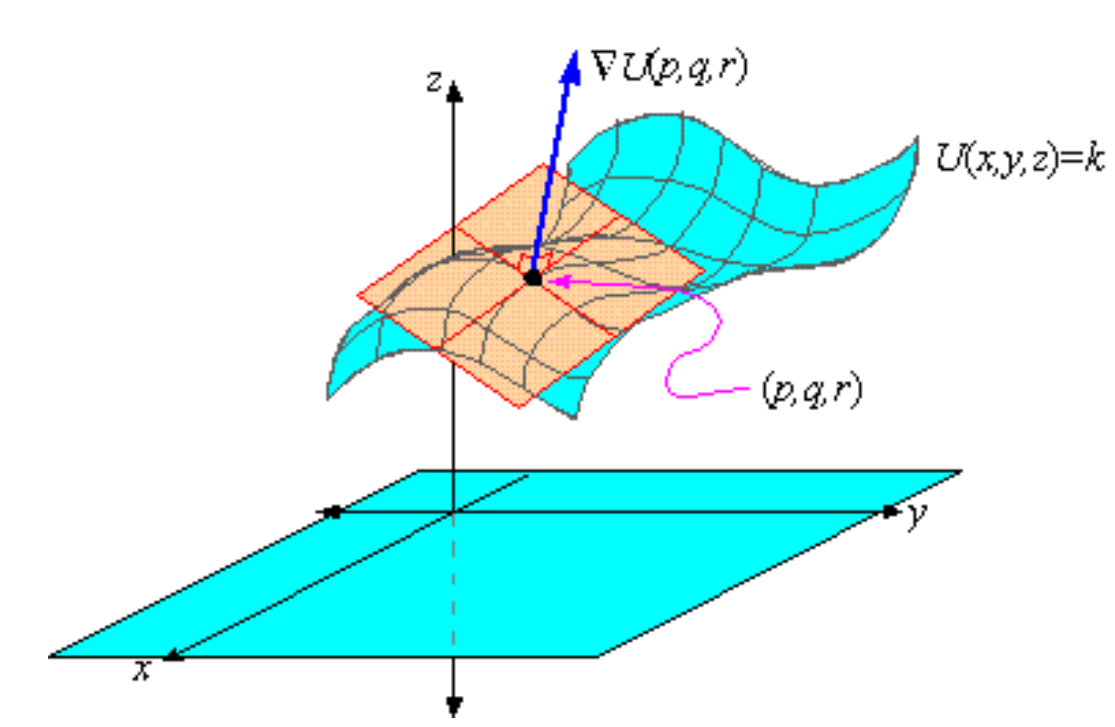
\includegraphics[height=5cm]{gradient_on_surface_2.PNG}
    \caption{Gradient is perpendicular to the local tangential plane.}
    \label{fig:gradient_on_surface}
\end{figure}



\newpage
\subsection{Taylor series for multi variable functions}
\label{app:taylor_multivar}

\begin{shaded*}
\begin{definition}
An $n$-times differentiable real function $f:\setR \rightarrow \setR$ can be expanded in the form of \emphasis{Taylor series} about a point $x=x_0$ as
\begin{equation}
f(x)=f(x_0) + f'(x_0)(x-x_0) + \frac{f''(x_0)}{2!}(x-x_0)^2 + \frac{f^{(3)}(x_0)}{3!}(x-x_0)^3 + \ldots + \frac{f^{(n)}(x_0)}{n!}(x-x_0)^n + \epsilon_n
\end{equation}
, where $\epsilon_n$ is the remainder or error polynomial. 
\end{definition}
\end{shaded*}
Therefore we can approximate the function $f$ using first order terms at $x_0$ as $f(x) \approx f(x_0) + f'(x_0)(x-x_0)$, using second order terms as $f(x) \approx f(x_0) + f'(x_0)(x-x_0) + \tfrac{f''(x_0)}{2!}(x-x_0)^2$, etc.\\
Alternatively, when $\Delta x$ is small, e.g. the 2nd degree approximation at $x=x_0 + \Delta x$ can be written as:
\[
f(x_0+\Delta x) \approx f(x_0) + f'(x_0)\Delta x + \frac{f''(x_0)}{2!}\Delta x^2 
\]
For a function of two independent variables $f(x,y)$, if we want to expand about $(x_0,y_0)$ using 2nd derivatives we take partial derivatives letting $f _x = \tfrac{\partial f}{\partial x},\ f _y = \tfrac{\partial f}{\partial y},\ x=x_0+\Delta x,\ y=y_0+\Delta y$ in the above form and have \cite{taylor_123}
\[
\begin{split}
f(x_0 + \Delta x,y_0+ \Delta y) \approx & f(x_0,y_0) + f_x \Delta x + f_y \Delta y +\\
										& f_{xx}(x_0,y_0)\frac{\Delta x^2}{2} + f_{yy}(x_0,y_0)\frac{\Delta y^2}{2} + f_{xy}(x_0,y_0)\Delta x \Delta y
\end{split}
\]
Equivalently, using the first form \cite{lec_notes_fsu}:
\[
\begin{split}
f(x,y) \approx & f(x_0,y_0) + f_x \cdot (x-x_0) + f_y \cdot (y-y_0) +\\
										& f_{xx}(x_0,y_0)\frac{(x-x_0)^2}{2} + f_{yy}(x_0,y_0)\frac{(y-y_0)^2}{2} + f_{xy}(x_0,y_0)(x-x_0)(y-y_0)
\end{split}
\]
A bit more elegantly, denoting the small displacements as $\Delta x := x-x_0,\ \Delta y := y - y_0$:
\begin{equation}
\begin{split}
f(x,y) \approx & f(x_0,y_0) + f_x \cdot \Delta x + f_y \cdot \Delta y +\\
										& \frac{1}{2} \left ( f_{xx}(x_0,y_0)\Delta x^2 + f_{yy}(x_0,y_0)\Delta y^2 + 2f_{xy}(x_0,y_0)\Delta x \Delta y \right )
\end{split}
\label{eq:taylor_multivar_Dx}
\end{equation}
We want to find a more compact matrix-based way to write the above equations deonoting our 2-variable function $f:\setR^2 \rightarrow \setR$ as $f(\B{x}),\ \B{x}=\begin{bmatrix}x & y \end{bmatrix}^T$ and seeking the 2nd order approximation around a fixed point $\B{x}_0 = \begin{bmatrix}x_0 & y_0 \end{bmatrix}$. From Section 1 we know that the sum $f_{xx}(x_0,y_0)\frac{(x-x_0)^2}{2} + f_{yy}(x_0,y_0)\frac{(y-y_0)^2}{2} + f_{xy}(x_0,y_0)(x-x_0)(y-y_0)$ can be written as a quadratic form, particularly:
\[
\begin{gathered}
f_{xx}(x_0,y_0)\frac{(x-x_0)^2}{2} + f_{yy}(x_0,y_0)\frac{(y-y_0)^2}{2} + f_{xy}(x_0,y_0)(x-x_0)(y-y_0) =\\ 
\frac{1}{2}(\B{x}-\B{x}_0)^T \begin{bmatrix}f_{xx}(\B{x}_0) & f_{xy}(\B{x}_0) \\f_{yx}(\B{x}_0) & f_{yy}(\B{x}_0)  \end{bmatrix} (\B{x} - \B{x}_0) = \\
\frac{1}{2}(\B{x}-\B{x}_0)^T \B{H}_f(\B{x}_0)(\B{x} - \B{x}_0) = 
\end{gathered}
\]
, where $\B{H}_f(\B{x}_0)$ is the Hessian matrix of $f$ at fixed point $\B{x}_0$.\\
Recall that the gradient of $f$ is $\nabla f = \begin{bmatrix}f_x & f_y \end{bmatrix}$ so the term can be written as the dot product $(\B{x} - \B{x}_0)^T \cdot \nabla f (\B{x}_0)$. 
\begin{corollary}
Putting everything together, the 2nd order Taylor approximation of a function $f:\setR^2 \rightarrow \setR$ or $f:\setRn \rightarrow \setR$ in general around a fixed point $\B{x}_0$ is
\begin{equation}
f(\B{x}) = f(\B{x}_0) + (\B{x} - \B{x}_0)^T \cdot \nabla f (\B{x}_0) + \frac{1}{2}(\B{x}-\B{x}_0)^T \B{H}_f(\B{x}_0)(\B{x} - \B{x}_0)
\label{eq:taylor_multivar}
\end{equation}
, where $\B{H}_f(\B{x}_0)$ is the Hessian matrix ($n \times n$) evaluated at $\B{x}_0$. The Hessian matrix is of course symmetric for any size as $f_{xy}=f_{yx}.$
\end{corollary}
The following result is now straightforward from \eqref{eq:taylor_multivar}.
\begin{corollary}
Let $f(x,y)$ be a twice differentiable function, and let $(x_0,y_0)$ be a critical point for $f$, i.e. $\nabla f(x_0,y_0)=0$.
\begin{enumerate}
\item If $\B{H}_f(x_0,y_0)$ is positive definite, then $x_0,y_0$ is a local minimum for $f$.
\item If $\B{H}_f(x_0,y_0)$ is negative definite, then $x_0,y_0$ is a local maximum for $f$.
\item If $\B{H}_f(x_0,y_0)$ is indefinite, then $x_0,y_0$ is a saddle point for $f$.
\end{enumerate}
\end{corollary}

\begin{proof}
\cite{stackexch_tay}~We know that at the critical point the gradient vanishes, i.e.
\[
\nabla f (x_0,y_0) = \B{0}
\]
So the 2nd order Taylor expansion at the critical point $\B{x}_0 = (x_0,y_0)$looks like
\[
f(\B{x}_0 + \Delta \B{x}) \approx f(\B{x}_0) + \frac{1}{2}\Delta \B{x}^T \B{H}_f(\B{x}_0) \Delta \B{x}
\tag{1}
\label{eq:taylor_2nd_order_extremum}
\]
Thus, for small displacements $\Delta x$, the Hessian tells us how the function behaves around the critical point.
\begin{enumerate}
\item If the Hessian is positive definite, then  $\Delta \B{x}^T \B{H}_f(\B{x}_0) \Delta \B{x} > 0$ therefore from \eqref{eq:taylor_2nd_order_extremum} we have $f(\B{x}_0 + \Delta \B{x}) > f(\B{x})$ around $\B{x}_0$. Then in every direction around that point $f(\B{x})$ grows thus $\B{x}_0$ is a local minimum.
\item If the Hessian is negative definite, then  $\Delta \B{x}^T \B{H}_f(\B{x}_0) \Delta \B{x} < 0$ therefore from \eqref{eq:taylor_2nd_order_extremum} we have $f(\B{x}_0 + \Delta \B{x}) < f(\B{x})$ around $\B{x}_0$, i.e. $\B{x}_0$. Then in every direction around that point $f(\B{x})$ shrinks thus $\B{x}_0$ is a local maximum.
\item If the Hessian is negative definite, then  there exists $\Delta \B{x} \neq \B{0}$ such that $\Delta \B{x}^T \B{H}_f(\B{x}_0) \Delta \B{x} = 0$. In this case the test fails; along this direction we aren't really sure whether the function $f$ is increasing or decreasing as we move away from $\B{x}_0$; our second order approximation isn't good enough and we need higher order data to decide.
\end{enumerate}
When considering the definitiveness of the Hessian, remember the equivalent definitiveness criteria from Theorems \ref{theorem:positive_def}, \ref{theorem:negative_definite}. We will use those to formulate an equivalent 2nd partial derivative extremum test.
\end{proof}

\begin{corollary}
Let $f$ be twice deffertiable with continuous second derivatives round $(x_0,y_0)$ and $(x_0,y_0)$ be a critical point, i.e. $\nabla f(x_0,y_0)=\B{0}$. The determinant of the Hessian is $det(\B{H}_f)(x_0,y_0) = f_{xx}f_{yy} - f_{xy}f_{yx} = f_{xx}f_{yy} - f_{xy}^2$.
\begin{enumerate}
\item If $det(\B{H}_f)(x_0,y_0) > 0$ and $f_{xx}>0$ then $x_0,y_0$ is a local minimum.
\item If $det(\B{H}_f)(x_0,y_0) > 0$ and $f_{xx}<0$ then $x_0,y_0$ is a local maximum.
\item If $det(\B{H}_f)(x_0,y_0) < 0$  then $x_0,y_0$ is a saddle point.
\item If $det(\B{H}_f)(x_0,y_0) = 0$  then the test is inconclusive and $(x_0,y_0)$ can be either a minimum, maximum, or saddle point.
\end{enumerate}
\end{corollary}
\begin{proof} \quad \\
\begin{enumerate}
\item From Theorem \ref{theorem:positive_def}, this proposition implies that the determinants of all upper left principal minors are positive (as $det(\B{H}_f)(x_0,y_0) > 0$ and $f_{xx}>0$ (which implies also $f_{yy}>0$) therefore $\B{H}_f(x_0,y_0)$ is positive definite, thus $x_0,y_0$ is a local minimum.
\item From Theorem \ref{theorem:negative_definite} this proposition implies that the determinants of all upper left principal minors have sign $(-1)^k$  as $det(\B{H}_f)(x_0,y_0) > 0$ and $f_{xx}<0$  (which implies also $f_{yy}>0$) therefore $\B{H}_f(x_0,y_0)$ is negative definite, thus $x_0,y_0$ is a local maximum.
\item If $det(\B{H}_f)(x_0,y_0) < 0$ then we have one positive and one negative eigenvalue therefore $\B{H}_f(x_0,y_0)$ is indefinite, thus $x_0,y_0$ is a saddle point.  
\end{enumerate}
An intuituve way to remember whether the sign of $f_{xx}$ combined with positive determinant implies minimum or maximum is to compare it with the 1D local minimum case.
\end{proof}
\begin{proof} \quad \\
\cite{lec_notes_jones} This is an alternative proof that does not consider the definitiveness criteria. From \eqref{eq:taylor_multivar_Dx} with $\Delta x = x - x_0,\ \Delta y = y - y_0$ around the critical point $(x_0,y_0)$, i.e. $\nabla f (x_0,y_0) = \B{0}$, we have
\[
\begin{split}
\Delta f &= f(x_0 + \Delta x, y_0 + \Delta y) - f(x_0,y_0)= \\
&= \frac{1}{2}\left[f_{xx}(\Delta x)^2 + f_{yy}(\Delta y)^2 + 2f_x f_y \Delta x \Delta y\right]
\end{split}
\tag{2}
\label{eq:taylor_multivar_Dx_Df}
\]
\textbf{Maximum:} What condition do we need for a local maximum? \\
For a maximum, all small steps away from $(x_0,y_0)$ will lead to $\Delta f < 0$ therefore \eqref{eq:taylor_multivar_Dx_Df} implies that
\[
f_{xx}(\Delta x)^2 + f_{yy}(\Delta y)^2 + 2f_x f_y \Delta x \Delta y < 0 
\tag{3}
\label{eq:taylor_multivar_Dx_Df_min_cond}
\]
for arbitary sufficiently small $\Delta x, \Delta y$. We can therefore set in \eqref{eq:taylor_multivar_Dx_Df_min_cond} $\Delta x = 0$, which yields:
\[
f_{xx} < 0
\tag{4}
\label{eq:taylor_multivar_Dx_Df_min_result_1}
\]
(Also similarly, $f_{yy}<0$.) We can also align the displacements as $\Delta x = \lambda \Delta y$, i.e. in \eqref{eq:taylor_multivar_Dx_Df_min_cond} set $(\Delta x, \Delta y) := (\lambda \Delta y, \Delta y)$, which yields:
\[
\lambda^2 f_{xx} + 2\lambda f_{xy} + f_{yy} < 0 \quad \forall \lambda \neq 0
\]
Multiplying by $f_{xx}$ (remember \eqref{eq:taylor_multivar_Dx_Df_min_result_1}) we obtain:
\[
\begin{split}
\lambda^2 f_{xx}^2 + 2\lambda f_{xy}f_{xx} + f_{yy}f_{xx} &> 0 \Rightarrow \\
f_{xy}^2 - f_{xx}f_{yy} &< (f_{xx}\lambda  + f_{xy})^2 \hquad \forall \hquad \lambda \neq 0
\end{split}
\tag{5}
\label{eq:taylor_multivar_Dx_Df_min_result_2}
\]
Picking $\lambda = -f_{xy}/f_{xx}$ we can set the right side to zero so we end up with:
\[
f_{xy}^2 - f_{xx}f_{yy} < 0
\tag{6}
\label{eq:taylor_multivar_Dx_Df_min_result_3}
\]
The conditions in \eqref{eq:taylor_multivar_Dx_Df_min_result_1} and \eqref{eq:taylor_multivar_Dx_Df_min_result_3} state that $(x_0,y_0)$ is a local maximum when:
\begin{align*}
f_{xx} < 0	& & \textup{and}& &	f_{xy}^2 - f_{xx}f_{yy} < 0 \Leftrightarrow\\
			& & & &	f_{xx}f_{yy} - f_{xy}^2 > 0 \Leftrightarrow\\
            & & & &	\textup{det}(\B{H}_f)(x_0,y_0) > 0\\
\tag{7}
\label{eq:taylor_multivar_Dx_Df_min_result_4}
\end{align*}
Using the Principal Minor equivalence criterior (Theorem \ref{theorem:negative_definite}), \eqref{eq:taylor_multivar_Dx_Df_min_result_4} implies that $\B{H}_f$ must be negative definite at at local maximum $(x_0,y_0)$.\\

\textbf{Minimum:} The same type of argument can be applied to formulate the condition for a minimum.

\textbf{Saddle point:} \\
For a saddle point, we'd have $\Delta f = 0$ in \eqref{eq:taylor_multivar_Dx_Df}. However, we don't know how $\Delta x$ and $\Delta y$ change as we move away from $(x_0,y_0)$. We can still set $\Delta x = \lambda \Delta y$ but $\lambda$ needs to be found. Again, from \eqref{eq:taylor_multivar_Dx_Df_min_cond} we have:
\[
\lambda^2f_{xx} + 2\lambda f_{xy} + f_{yy} = 0
\tag{8}
\label{eq:taylor_multivar_saddle_res_1}
\]
This implies that there are only two direction $\lambda_1, \lambda_2$ for which $\Delta x = \lambda_i \Delta y$ obtained by solving the above equation. Multiplying by $f_{xx}$ and completing the square:
\[
\begin{gathered}
\lambda^2 f_{xx}^2 + 2\lambda f_{xy} f_{yy} + f_{yy}^2 = f_{yy}^2 -f_{xx}f_{yy} \Rightarrow\\
(\lambda f_{xx}+ f_{yy})^2 = f_{xy}^2 -f_{xx}f_{yy}
\end{gathered}
\]
Because $\lambda$ solves \eqref{eq:taylor_multivar_saddle_res_1}, it cannot satisfy $(\lambda f_{xx}+ f_{yy})^2 = 0$ at the same time therefore 
\[
\begin{gathered}
(\lambda f_{xx}+ f_{yy})^2 > 0 \Rightarrow 
 f_{xy}^2 -f_{xx}f_{yy} > 0
 \tag{9}
 \label{eq:taylor_multivar_saddle_res_2}
\end{gathered}
\]
To sum up, the condition for saddle point at $(x_0,y_0)$ is given by \eqref{eq:taylor_multivar_saddle_res_2}.
\end{proof}







\newpage
\subsection{Intuition behind Lagrange multiplier}


\TODO[maybe in the future] \\
\url{https://www.reddit.com/r/math/comments/g4w7m/can_anyone_provide_a_concise_and_intuitive/}\\
\url{https://ocw.mit.edu/courses/mathematics/18-02sc-multivariable-calculus-fall-2010/2.-partial-derivatives/part-c-lagrange-multipliers-and-constrained-differentials/session-40-proof-of-lagrange-multipliers/MIT18_02SC_notes_22.pdf}\\
\url{http://www.uoguelph.ca/economics/repec/workingpapers/2010/2010-03.pdf}\\




\newpage
\subsection{Relationship between rank and number of non-zero eigenvalues}
\label{app:rank_eigevalues}

The relationship is derived in a number of sets and a special case holds for symmetric matrices.
\begin{itemize}
\item Eigenvectors of distinct eigenvalues are lin. ind.
\item Eigenvectors of nonzero eigenvalues of $\B{A}$ are in its column space (or range) $\mathcal{R}\left(\B{A}\right)$ as $\B{v}_i = \B{A}\B{v}_i/\lambda_i$ is a combination of $\B{A}$'s columns.
\item Therefore, if $r:=\textup{rank}(\B{A})$ and we have $k$ (not necessarily distinct) eigenvalues, then $k \leq r$. Also for the null space, $\textup{dim}\left(\mathcal{N}(\B{A})\right) = n - r \geq n - k$.
\item If $\B{A}$ is \textit{symmetric}, all its eigenvalues are distinct therefore all its eigenvectors are lin. ind. so their number equals the dimension of their spanning set, i.e. $k = \textup{dim}\left(\textup{span}\{\B{v}_1,\ldots,\B{v}_k\}\right)$. But each eigenvector is in the column space of $\B{A}$ so it follows $k = r = \rank(\B{A})$. Also, then $\dim \left(\mathcal{N}(\B{A})\right) = n - k$. Remember that for the null space $\B{A}\B{v} = 0 \cdot \B{v}$ so its dimension is equal to the number of zero eigenvalues of the symmetric matrix $\B{A}$.
\end{itemize}


\newpage
\subsection{Why do orthogonal matrices represent rotations?}
\label{app:orthog_and_rotations}

\TODO[soon, more urgent] \\
\url{https://math.stackexchange.com/questions/612936/why-are-orthogonal-matrices-generalizations-of-rotations-and-reflections}\\
\url{https://www.quora.com/Why-do-orthogonal-matrices-represent-rotations/answer/Julius-Bier-Kirkegaard}


\newpage
\subsection{Matlab program to compress image by using SVD}
\label{app:svd_matlab}

\inputminted{octave}{svd_compr.m}
The file generated storing the results is listed below. Note how the result confirm the Eckart-Young-Mirsky theorem \ref{theorem:svd_best_approx}.
\begin{verbatim}
rank, number of elements required, compression ratio, norm2(A-A_k), sigma_(k+1)
1,513,0.0078278,28.3839,28.3839
2,1026,0.015656,21.5064,21.5064
10,5130,0.078278,6.0213,6.0213
20,10260,0.15656,3.5956,3.5956
32,16416,0.25049,2.379,2.379
64,32832,0.50098,1.1571,1.1571
\end{verbatim}






\newpage
\subsection{Linear least squares solution}
\label{app:least_squares}

Let's say that we suppose a body is moving roughly in a straight line $y = bx + a$ have measured its position at various points $(x_1,y_1),(x_2,y_2),\ldots, (x_k,y_k)$. Ideally, we'd want $y_i = bx_i + a \hquad \forall i: \hquad 1 \leq i \leq n$ to be true. Unless vectors $(x_1,y_1),(x_2,y_2),\ldots, (x_k,y_k)$ are all l.i., $a + bx_i = y_i, 1 \leq i \leq k$ is impossible to solve as we have more equations than unknowns, or equivalently the system $\B{A}_{m\times n}\B{x}=\B{b}, \hquad \B{A}=\begin{bmatrix}1 & x_1 \\ \cdots & \cdots \\ 1 & x_k \end{bmatrix}, \hquad \B{x}=\begin{bmatrix}a \\ b \end{bmatrix}, \hquad \B{y}=\begin{bmatrix}y_1 \\ \ldots \\ y_k \end{bmatrix}$ is \emphasis{overdetermined}. That follows from the fact that the rows of $\B{A}$ are l.i. and that $m=k>n=2$. \\
To summarise, when $\B{A}_{m \times n} \B{u} = \B{b}, \hquad m>n$ and we have to solve the "tall and skinny" system
\[
\begin{bmatrix}a_{11} & \ldots & a_{1n}\\ \vdots & \ddots & \vdots\\ a_{m1} & \ldots & a_{mn}\\ \end{bmatrix}
\begin{bmatrix}u_1 \\ \vdots \\u_n \end{bmatrix} = 
\begin{bmatrix}b_1 \\ \vdots b_m \end{bmatrix}
\]
, where $\B{A}$ has more than n l.i. rows, then $\B{A}^{-1}$ does not exist and there are no solutions. It is impossible to write $\B{b} \in \setR^m$ as a linear combination of the columns of $\B{A}$. However, the column space of $\B{A}$ is in $\setR^ 2$. Instead, we want to find the best approximation of $\B{b}$ in $\setR^2$.


\begin{exmp}
ref: \url{https://www.cs.auckland.ac.nz/courses/compsci369s1c/lectures/GG-notes/CS369-LeastSquares.pdf} \\
(Linear regression in statistics) Try to fit the measurements $(0,1),(1,9),(3,9), (4,21)$ in a straight line.
\end{exmp}
\begin{TheSolution}
Let the straight line be $b_i = u_1 + u_2x_i$, then we'd have to solve
\[
\begin{bmatrix}
1 & 0\\
1 & 1\\
1 & 3\\
1 & 4 
\end{bmatrix}
\begin{bmatrix}
u_1 \\ u_2
\end{bmatrix}
=
\begin{bmatrix}
1 \\ 9 \\ 9 \\ 21
\end{bmatrix}
\]
The above equation does not have a solution as $\begin{bmatrix}
1 & 9 & 9 & 21
\end{bmatrix}^T$ cannot be written as a linear combination of $\begin{bmatrix}1 & 0 \end{bmatrix}^T, \hquad  \begin{bmatrix}1 & 1 \end{bmatrix}^T, \hquad  \begin{bmatrix}1 & 3 \end{bmatrix}^T, \hquad \begin{bmatrix}1 & 4 \end{bmatrix}^T$. \TODO[insert graph here] \qedblack
\end{TheSolution}

\url{https://www.cs.auckland.ac.nz/courses/compsci369s1c/lectures/GG-notes/CS369-LeastSquares.pdf}\\
The way we work is find a straight line $y=u_1+u_2x$ such that the magnitude of the error vector $ \B{e} = \begin{bmatrix}e_1 & \ldots & e_m \end{bmatrix} = \begin{bmatrix}y_1 - u_1 - u_2x_1 & \ldots & y_m - u_1 - u_2x_m\end{bmatrix}, \hquad \norm{\B{e}} = e_1^2 + \ldots + e_m^2 = (y_1 - u_1 - u_2x_1)^2 + \ldots +  (y_m - u_1 - u_2x_m)^2 $ is minimised (hence the "least squares"). In general, when solving the overdetermined system $\B{A}\B{u}=\B{b}$, the error vector is given by
\begin{equation}
\B{e}=\B{b} - \B{A}\bar{\B{x}}
\end{equation}
, where $\bar{\B{x}}$ minimises the magnitude of $\B{e}$. We will prove the following theorem for the least squares solution.

\begin{shaded*}
\begin{theorem}
Let $\B{A}$ be an $m \times n$ matrix and let $\B{b} \in \setR^m$. Then $\B{Ax}=\B{b}$ always has at least one least squares solution $\bar{\B{x}}$. The following properties hold:
\begin{enumerate}
\item $\bar{\B{x}}$ is a least squares solution of $\B{A}\bar{\B{x}}=\B{b}$ iff $\bar{\B{x}}$ is a solution of the \textup{\emphasis{normal equations}}
\begin{equation}
\left(\B{A}^T\B{A} \right)\bar{\B{x}} = \B{A}^T\B{b}
\end{equation}
\item \B{A} has linearly independent columns if and only if $\B{A}^T\B{A}$ is invertible. In this case, the least squares solution of $\B{Ax}=\B{b}$ is unique and is given by
\begin{equation}
\bar{\B{x}} =\left(\B{A}^T\B{A} \right)^{-1} \B{A}^T\B{b}
\end{equation}
\end{enumerate}
\end{theorem}
\end{shaded*}

\begin{proof}
To prove the theorem, we suppose we want to a vector in $\setR^3$ in a 2D plane but what we'll prove holds in general. We want to approximate the $\B{b}$ vector as $\B{A}\bar{\B{x}}$ in the $\B{A}\B{x}$ plane, i.e. in the column space of $\B{A}$ such that the magnitude of $\B{e} = \B{b}\B{A}\bar{\B{x}}$ is minimsed. In the figure below one can see (Pythagoras) the best approximation of $\B{b}$is its projection $\B{p}=\textup{proj}_{\fancyR(\B{A})}\B{b}=\B{A}\B{u}$. 
\begin{figure}[H]
	\centering %centralizar a figura
	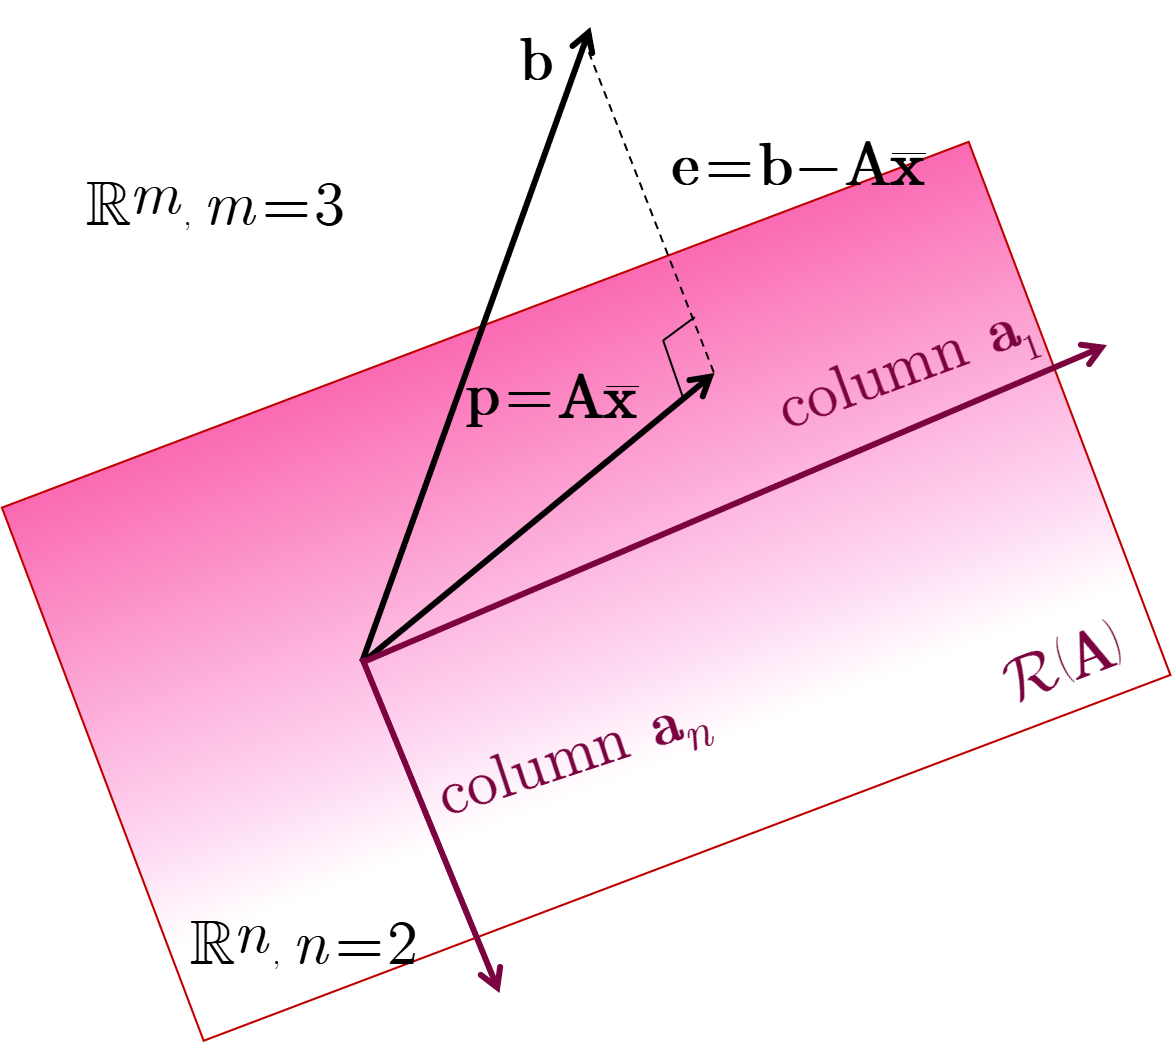
\includegraphics[height=5cm]{least_sq_proj.png}
    \caption{Approximating a 3D vectors in a 2D space by using its projection.}
    \label{fig:least_sq_proj}
\end{figure}
To minimise the length of $\B{e}$, it must be perpendicular to the column space $\fancyR(\B{A})$, therefore ("fundamental theorem of linear algebra") it must lie in the left nullspace of $\B{A}$, $\fancyN(\B{A}^T)$, i.e. such that $\B{A}^T\B{e}=0$. Alternatively, writing $\B{A}$ in columns as $\B{A}=\begin{bmatrix}\B{a}_1 & \ldots & \B{a}_n \end{bmatrix}$, we could express the orthogonalirt as the dot product constraints
\[
\begin{gathered}
\B{a}_1^T \B{e} = 0 \\
\ldots \\
\B{a}_n^T \B{e} = 0 \Rightarrow\\
\B{A}^T\B{e}=0
\end{gathered}
\]

Either way, we end up with:

\[
\begin{gathered}
\B{A}^T\B{e}=0 \Rightarrow \\
\B{A}^T(\B{b} - \B{A}\bar{\B{x}}) = 0 \Rightarrow \\
\B{A}^T \B{A}\bar{\B{x}} =  \B{A}^T\B{b} 
\end{gathered}
\]
Hence the normal equations are derived.
\end{proof}

\begin{proof} (Part 2, $\Rightarrow$)
We want to know when $\B{A}^T \B{A}\bar{\B{x}} =  \B{A}^T\B{b} $ can be solved for $\bar{\B{x}}$, i.e. when $\B{A}^T\B{A}$ is invertible. Suppose $\B{A}$ has l.i. columns. We want to show that $\B{A}^T\B{A}$ is invertible, or equivalently that the nullspace of $\B{A}^T\B{A}$  is $\B{0}$, i.e suppose
\[
\B{A}^T\B{A}\B{x} = \B{0}
\tag{1}
\label{eq:l_sq_proof_1}
\]
Then we want to show that \eqref{eq:l_sq_proof_1} holds only for $\B{x}=\B{0}$. $\B{Ax}\in \fancyR(\B{A})$ therefore it is orthogonal to the left nullspace of $\B{A}$. From \eqref{eq:l_sq_proof_1} we also have that $ \B{A}\bar{\B{x}}$ is in the left null space of $\B{A}$. These two conditions can only hold if the vector is zero:
\[
\B{Ax} = 0
\]
Since $\B{A}$'s columns are l.i. it is invertible therefore $\B{x}=\B{0}$.
\end{proof}
\begin{proof} (Part 2, $\Leftarrow$)
Suppose $\B{A}^T\B{A}$ is invertible, then we want to show that $\B{A}$ is invertible too. We first show that the null spaces of $\B{A}^T\B{A}$ and $\B{A}$ are equal (left as exercise) therefore:
\[
\begin{split}
\fancyN(\B{A}^T\B{A}) &= \fancyN(\B{A}) \Rightarrow \\
\dim\left(\fancyN(\B{A}^T\B{A})\right) &= \dim \left( \fancyN(\B{A})\right) \Rightarrow \\
\rank\left(\fancyN(\B{A}^T\B{A})\right) &= \rank \left( \fancyN(\B{A})\right)  
\end{split}
\]
\end{proof}
The projection of $\B{x}$ in the column space of $\B{A}$ is
\[
\B{p} = \B{A}\bar{\B{x}} = \B{A}\left(\B{A}^T\B{A} \right)^{-1} \B{A}^T\B{b}
\]
Matrix $\B{A}\bar{\B{x}} = \B{A}\left(\B{A}^T\B{A} \right)^{-1} \B{A}^T$ is called \emphasis{projection matrix}. $\B{Ax}=\B{b}$ has no solution but  $\B{Ax}=\B{p}$ has a solution $\bar{\B{x}}$.
\begin{corollary} \quad \\
\begin{enumerate}
\item The projection matrix $\B{P} = \B{A}\bar{\B{x}} = \B{A}\left(\B{A}^T\B{A} \right)^{-1} \B{A}^T\B{b}$ is symmetric.
\item $\B{P}^2 = \B{P}$, as repeated projections give the same result.
\item $\B{P}$ is $m \times m$ but of rank only $n$.
\end{enumerate}

\end{corollary}





\newpage
\subsection{Pseudoinverse with QR factorisation}
\label{app:pseudo_with_qr}

\TODO \\
\url{https://see.stanford.edu/materials/lsoeldsee263/05-ls.pdf}





\newpage
%usepackagebiblatex[...]
\printbibliography

\end{document}
